% Options for packages loaded elsewhere
\PassOptionsToPackage{unicode}{hyperref}
\PassOptionsToPackage{hyphens}{url}
%
\documentclass[
]{article}
\usepackage{amsmath,amssymb}
\usepackage{lmodern}
\usepackage{iftex}
\ifPDFTeX
  \usepackage[T1]{fontenc}
  \usepackage[utf8]{inputenc}
  \usepackage{textcomp} % provide euro and other symbols
\else % if luatex or xetex
  \usepackage{unicode-math}
  \defaultfontfeatures{Scale=MatchLowercase}
  \defaultfontfeatures[\rmfamily]{Ligatures=TeX,Scale=1}
\fi
% Use upquote if available, for straight quotes in verbatim environments
\IfFileExists{upquote.sty}{\usepackage{upquote}}{}
\IfFileExists{microtype.sty}{% use microtype if available
  \usepackage[]{microtype}
  \UseMicrotypeSet[protrusion]{basicmath} % disable protrusion for tt fonts
}{}
\makeatletter
\@ifundefined{KOMAClassName}{% if non-KOMA class
  \IfFileExists{parskip.sty}{%
    \usepackage{parskip}
  }{% else
    \setlength{\parindent}{0pt}
    \setlength{\parskip}{6pt plus 2pt minus 1pt}}
}{% if KOMA class
  \KOMAoptions{parskip=half}}
\makeatother
\usepackage{xcolor}
\usepackage[margin=1in]{geometry}
\usepackage{graphicx}
\makeatletter
\def\maxwidth{\ifdim\Gin@nat@width>\linewidth\linewidth\else\Gin@nat@width\fi}
\def\maxheight{\ifdim\Gin@nat@height>\textheight\textheight\else\Gin@nat@height\fi}
\makeatother
% Scale images if necessary, so that they will not overflow the page
% margins by default, and it is still possible to overwrite the defaults
% using explicit options in \includegraphics[width, height, ...]{}
\setkeys{Gin}{width=\maxwidth,height=\maxheight,keepaspectratio}
% Set default figure placement to htbp
\makeatletter
\def\fps@figure{htbp}
\makeatother
\setlength{\emergencystretch}{3em} % prevent overfull lines
\providecommand{\tightlist}{%
  \setlength{\itemsep}{0pt}\setlength{\parskip}{0pt}}
\setcounter{secnumdepth}{-\maxdimen} % remove section numbering
\usepackage{multirow}
\usepackage{multicol}
\usepackage{colortbl}
\usepackage{hhline}
\newlength\Oldarrayrulewidth
\newlength\Oldtabcolsep
\usepackage{longtable}
\usepackage{float}
\usepackage{wrapfig}
\usepackage{array}
\usepackage{hyperref}
\ifLuaTeX
  \usepackage{selnolig}  % disable illegal ligatures
\fi
\IfFileExists{bookmark.sty}{\usepackage{bookmark}}{\usepackage{hyperref}}
\IfFileExists{xurl.sty}{\usepackage{xurl}}{} % add URL line breaks if available
\urlstyle{same} % disable monospaced font for URLs
\hypersetup{
  pdftitle={Orange Dot Report 5.0},
  pdfauthor={Ridge Schuyler, Michele Claibourn, Lee LeBoeuf, Elizabeth Mitchell},
  hidelinks,
  pdfcreator={LaTeX via pandoc}}

\title{Orange Dot Report 5.0}
\usepackage{etoolbox}
\makeatletter
\providecommand{\subtitle}[1]{% add subtitle to \maketitle
  \apptocmd{\@title}{\par {\large #1 \par}}{}{}
}
\makeatother
\subtitle{Family Self-Sufficiency in the Charlottesville Region}
\author{Ridge Schuyler, Michele Claibourn, Lee LeBoeuf, Elizabeth
Mitchell\footnote{\textbf{Ridge Schuyler}, Dean, Division of Community
  Self-Sufficiency Programs - Network2Work@PVCC, Piedmont Virginia
  Community College, originated the Orange Dot Report in 2011 and has
  authored three prior updates (2015, 2018, 2021). This year begins a
  partnership with The Equity Center at the University of Virginia to
  support the ongoing updates, authorship, and expansion of this work.
  \textbf{Michele Claibourn}, Director of Equitable Analysis, The Equity
  Center, University of Virginia and Assistant Professor, Batten School
  of Leadership and Public Policy, University of Virginia. \textbf{Lee
  LeBoeuf}, Research Data Fellow, The Equity Center, University of
  Virginia and Ph.D.~Candidate, Department of Psychology, University of
  Virginia. \textbf{Elizabeth Mitchell}, Research Programs Manager, The
  Equity Center, University of Virginia.}}
\date{October 27, 2022}

\begin{document}
\maketitle

\hypertarget{preface}{%
\subsection{Preface}\label{preface}}

The first Orange Dot Report was released in 2011, and it served both to
describe the local income deficit---the gap between what families
receive as income and what they need to earn to be self-sufficient---in
Charlottesville and to develop strategies for creating pathways to
self-sufficiency for families in the region. This initial effort
launched the innovative Network2Work framework pioneered at Piedmont
Virginia Community College, a process that brings together a Job-Seeker
Network, an Employer Network, and a Provider Network to match
job-seekers to family-sustaining jobs and careers and to connect them to
community resources using neighborhood-based volunteers.

As Network2Work has grown, the Orange Dot Report has also expanded,
encompassing Charlottesville and Albemarle County in Orange Dot Report
2.0 (2015) and the entire region (Albemarle, Buckingham,
Charlottesville, Fluvanna, Greene, Louisa, and Nelson) in Orange Dot
Report 3.0 (2018) and Orange Dot Report 4.0 (2021). Along the way, the
report has come to serve as a central resource for the community and an
important update on the progress of our community.

This effort, Orange Dot Report 5.0, represents the continuation of our
progress toward a more fully and equitable thriving region.
Incorporating an updated description of the condition of families in our
larger region, Orange Dot 5.0 marks the beginning of an annual update
completed in partnership between Network2Work@PVCC and The Equity Center
at the University of Virginia. We will be providing an update of the
report in early spring incorporating the most recent information from
the U.S. Census' American Community Survey along with more assessment of
community efforts and progress in creating realistic pathways to
self-sufficiency.

\hypertarget{summary}{%
\subsection{Summary}\label{summary}}

In the larger Charlottesville community, 9,413 families (14\%) do not
make enough money to afford the essentials of life---food, shelter,
clothing and utilities---and the added costs associated with
working---childcare and transportation. This number represents the
families making less than \$35,000 in our region.

This is a significant improvement since the first Orange Dot Report in
2011. For the Charlottesville region, defined here as the city of
Charlottesville and the surrounding counties of Albemarle, Buckingham,
Fluvanna, Greene, Louisa and Nelson, the comparable number of families
struggling in the region in 2011 was 12,552, which was 21\% of families.
Over one out of five families. \textbf{The 2022 number--9,413
families--is a 25\% reduction in the number of struggling families in
the region.}

We recognize, however, that the cost of essentials has gone up over
time. For example, these basic needs currently require over \$45,000 a
year for a single parent with a toddler in childcare.\footnote{Assuming
  all families in the region match this ``model'' family type, 20\% of
  the families would fall below this higher threshold} In this report,
we continue to use the \$35,000 income threshold as the break point for
defining struggling families to remain consistent with the four prior
reports, so these numbers should be understood as a minimum--at least
9,413 families are struggling.

While families facing economic insecurity live throughout our region,
the likelihood that a family is struggling varies by race and by place.
The struggle is not equally shared.

\begin{itemize}
\tightlist
\item
  Thirty-two percent of Black families make less than \$35,000 a year,
  compared to 11\% of white families, a persistent gap resulting from
  past and ongoing policies that suppress investment, opportunity, and
  wealth creation in Black communities.
\item
  The percent of families struggling overall is highest in Buckingham
  County, at 28\%, and lowest in Louisa County, at 8\%.
\item
  Within every locality except Fluvanna, there are neighborhoods where a
  quarter or more of families have less than family-sufficient incomes.
  The four neighborhoods with the highest percent of struggling families
  are in the city of Charlottesville.
\end{itemize}

Our community has seen progress since this work began in 2011, but there
are still too many struggling families. For a region as prosperous as
ours, however, ten thousand families is not too many to help.

\hypertarget{introduction}{%
\subsection{Introduction}\label{introduction}}

\begin{quote}
``{[}W{]}henever you are engaged in work that serves humanity and is for
the building of humanity, it has dignity, and it has worth {[}\ldots{]}
All labor has dignity.''

--- Martin Luther King Jr.\footnote{Martin Luther King, Jr.~(March 18,
  1968). Retrieved from
  \url{https://www.beaconbroadside.com/broadside/2018/03/the-50th-anniversary-of-martin-luther-king-jrs-all-labor-has-dignity.html}}
\end{quote}

The last few years have brought our country's and our community's
ongoing struggles and inequities into stark relief. The continued
pandemic, the growing housing affordability crisis, the increasing
volatility of man-made climate change have created challenges for all of
us. But low-income individuals, especially individuals of color, are
suffering disproportionately, both physically and financially.

Despite working hard, too many families struggle to make ends meet, in
part because their work is not treated with dignity. Or at least, their
labor is not valued as though their work has dignity. While the enormous
value, the essentialness, of the labor performed by ``front-line''
workers became clear to all during the pandemic, many people laboring in
these positions do not earn enough to provide for their families. For
example, the so-called ``caring economy''---childcare workers, home
health aides, teachers---provides enormous social value, but is not
given market value. Rising prices and inflation will only worsen the
strain.

We all seek security and stability: to feed our families, to see our
children thrive, to create community with others, to promote our
wellbeing. For families experiencing economic insecurity, all of this is
jeopardized. When faced daily with financial struggles---to pay for
housing, to repair the car that carries you to work, to put food on the
table, to find and afford a safe environment for your children---it is
difficult to be the parent you want to be, the worker you know you could
be, or the person you were meant to be. We all deserve a chance to
thrive, but we are all not yet given that chance. Towards that end, we
must seek to build an equitable economy, one intentionally constructed
on a foundation of racial justice.

Knowing that we can only solve issues we can understand, we provide a
snapshot of the families in our community who are struggling, an update
to the Orange Dot Project report first issued in September
2011.\footnote{To find previous versions of the Orange Dot report, go to
  \url{https://www.pvcc.edu/history-network2workpvcc-program}}

What we have learned since this work began in 2011 is that there are too
many struggling families in our community, but not too many to help.

\hypertarget{struggling-families}{%
\subsection{Struggling Families}\label{struggling-families}}

There are 66,633 families living in the Charlottesville region, defined
as the city of Charlottesville and the surrounding counties of
Albemarle, Louisa, Nelson, Buckingham, Greene, and Fluvanna.\footnote{Family
  is defined as two or more people related by birth, marriage, or
  adoption and living in the same household. U.S. Census Bureau (2020).
  Household Type, 2016-2020. Retrieved from
  \url{https://data.census.gov/cedsci/table?q=B11001\&g=0500000US51003,51029,51065,51079,51109,51125,51540\&tid=ACSDT5Y2020.B11001}.}

Of these, 9,413 families (14\%) do not make enough money to afford the
essentials of life---food, shelter, clothing and utilities---and the
added costs associated with working (childcare and
transportation).\footnote{This report reflects the U.S. Census Bureau's
  American Community Survey 5-year averages, 2016-2020.}

While this is still too many families, this is a decrease compared to
the numbers provided in the prior report just two years ago. In the
Orange Dot Report 4.0, there were 10,940 families (17\%) who did not
earn enough to meet their basic needs. Since then our community has seen
that number reduced by nearly fourteen percent.\footnote{This is a
  community success, brought about primarily by the hard work of the
  job-seekers themselves, made possible by the quality employers who
  hired them, and propelled by the social and material support supplied
  by family, friends and a network of community-based organizations and
  agencies.}

\hypertarget{number-of-families-struggling-in-the-region}{%
\subsubsection{Number of Families Struggling in the
Region}\label{number-of-families-struggling-in-the-region}}

\global\setlength{\Oldarrayrulewidth}{\arrayrulewidth}

\global\setlength{\Oldtabcolsep}{\tabcolsep}

\setlength{\tabcolsep}{0pt}

\renewcommand*{\arraystretch}{1.5}



\providecommand{\ascline}[3]{\noalign{\global\arrayrulewidth #1}\arrayrulecolor[HTML]{#2}\cline{#3}}

\begin{longtable}[c]{|p{5.00in}|p{5.00in}|p{5.00in}}



\hhline{>{\arrayrulecolor[HTML]{666666}\global\arrayrulewidth=2pt}->{\arrayrulecolor[HTML]{666666}\global\arrayrulewidth=2pt}->{\arrayrulecolor[HTML]{666666}\global\arrayrulewidth=2pt}-}

\multicolumn{1}{>{\cellcolor[HTML]{FFFFFF}\centering}p{\dimexpr 5in+0\tabcolsep}}{\textcolor[HTML]{000000}{\fontsize{11}{11}\selectfont{Locality}}} & \multicolumn{1}{>{\cellcolor[HTML]{FFFFFF}\centering}p{\dimexpr 5in+0\tabcolsep}}{\textcolor[HTML]{000000}{\fontsize{11}{11}\selectfont{Number\ of\ Families\ Struggling}}} & \multicolumn{1}{>{\cellcolor[HTML]{FFFFFF}\centering}p{\dimexpr 5in+0\tabcolsep}}{\textcolor[HTML]{000000}{\fontsize{11}{11}\selectfont{Percent\ of\ Families\ Struggling}}} \\

\noalign{\global\arrayrulewidth 0pt}\arrayrulecolor[HTML]{000000}

\hhline{>{\arrayrulecolor[HTML]{666666}\global\arrayrulewidth=2pt}->{\arrayrulecolor[HTML]{666666}\global\arrayrulewidth=2pt}->{\arrayrulecolor[HTML]{666666}\global\arrayrulewidth=2pt}-}\endhead



\multicolumn{1}{>{\cellcolor[HTML]{FFFFFF}\centering}p{\dimexpr 5in+0\tabcolsep}}{\textcolor[HTML]{000000}{\fontsize{11}{11}\selectfont{Albemarle}}} & \multicolumn{1}{>{\cellcolor[HTML]{FFFFFF}\centering}p{\dimexpr 5in+0\tabcolsep}}{\textcolor[HTML]{000000}{\fontsize{11}{11}\selectfont{2,614}}} & \multicolumn{1}{>{\cellcolor[HTML]{FFFFFF}\centering}p{\dimexpr 5in+0\tabcolsep}}{\textcolor[HTML]{000000}{\fontsize{11}{11}\selectfont{9.9\%}}} \\

\noalign{\global\arrayrulewidth 0pt}\arrayrulecolor[HTML]{000000}

\hhline{>{\arrayrulecolor[HTML]{BEBEBE}\global\arrayrulewidth=1pt}->{\arrayrulecolor[HTML]{BEBEBE}\global\arrayrulewidth=1pt}->{\arrayrulecolor[HTML]{BEBEBE}\global\arrayrulewidth=1pt}-}



\multicolumn{1}{>{\cellcolor[HTML]{FFFFFF}\centering}p{\dimexpr 5in+0\tabcolsep}}{\textcolor[HTML]{000000}{\fontsize{11}{11}\selectfont{Buckingham}}} & \multicolumn{1}{>{\cellcolor[HTML]{FFFFFF}\centering}p{\dimexpr 5in+0\tabcolsep}}{\textcolor[HTML]{000000}{\fontsize{11}{11}\selectfont{1,136}}} & \multicolumn{1}{>{\cellcolor[HTML]{FFFFFF}\centering}p{\dimexpr 5in+0\tabcolsep}}{\textcolor[HTML]{000000}{\fontsize{11}{11}\selectfont{28.1\%}}} \\

\noalign{\global\arrayrulewidth 0pt}\arrayrulecolor[HTML]{000000}

\hhline{>{\arrayrulecolor[HTML]{BEBEBE}\global\arrayrulewidth=1pt}->{\arrayrulecolor[HTML]{BEBEBE}\global\arrayrulewidth=1pt}->{\arrayrulecolor[HTML]{BEBEBE}\global\arrayrulewidth=1pt}-}



\multicolumn{1}{>{\cellcolor[HTML]{FFFFFF}\centering}p{\dimexpr 5in+0\tabcolsep}}{\textcolor[HTML]{000000}{\fontsize{11}{11}\selectfont{Charlottesville}}} & \multicolumn{1}{>{\cellcolor[HTML]{FFFFFF}\centering}p{\dimexpr 5in+0\tabcolsep}}{\textcolor[HTML]{000000}{\fontsize{11}{11}\selectfont{1,710}}} & \multicolumn{1}{>{\cellcolor[HTML]{FFFFFF}\centering}p{\dimexpr 5in+0\tabcolsep}}{\textcolor[HTML]{000000}{\fontsize{11}{11}\selectfont{19.1\%}}} \\

\noalign{\global\arrayrulewidth 0pt}\arrayrulecolor[HTML]{000000}

\hhline{>{\arrayrulecolor[HTML]{BEBEBE}\global\arrayrulewidth=1pt}->{\arrayrulecolor[HTML]{BEBEBE}\global\arrayrulewidth=1pt}->{\arrayrulecolor[HTML]{BEBEBE}\global\arrayrulewidth=1pt}-}



\multicolumn{1}{>{\cellcolor[HTML]{FFFFFF}\centering}p{\dimexpr 5in+0\tabcolsep}}{\textcolor[HTML]{000000}{\fontsize{11}{11}\selectfont{Fluvanna}}} & \multicolumn{1}{>{\cellcolor[HTML]{FFFFFF}\centering}p{\dimexpr 5in+0\tabcolsep}}{\textcolor[HTML]{000000}{\fontsize{11}{11}\selectfont{559}}} & \multicolumn{1}{>{\cellcolor[HTML]{FFFFFF}\centering}p{\dimexpr 5in+0\tabcolsep}}{\textcolor[HTML]{000000}{\fontsize{11}{11}\selectfont{7.8\%}}} \\

\noalign{\global\arrayrulewidth 0pt}\arrayrulecolor[HTML]{000000}

\hhline{>{\arrayrulecolor[HTML]{BEBEBE}\global\arrayrulewidth=1pt}->{\arrayrulecolor[HTML]{BEBEBE}\global\arrayrulewidth=1pt}->{\arrayrulecolor[HTML]{BEBEBE}\global\arrayrulewidth=1pt}-}



\multicolumn{1}{>{\cellcolor[HTML]{FFFFFF}\centering}p{\dimexpr 5in+0\tabcolsep}}{\textcolor[HTML]{000000}{\fontsize{11}{11}\selectfont{Greene}}} & \multicolumn{1}{>{\cellcolor[HTML]{FFFFFF}\centering}p{\dimexpr 5in+0\tabcolsep}}{\textcolor[HTML]{000000}{\fontsize{11}{11}\selectfont{791}}} & \multicolumn{1}{>{\cellcolor[HTML]{FFFFFF}\centering}p{\dimexpr 5in+0\tabcolsep}}{\textcolor[HTML]{000000}{\fontsize{11}{11}\selectfont{14.7\%}}} \\

\noalign{\global\arrayrulewidth 0pt}\arrayrulecolor[HTML]{000000}

\hhline{>{\arrayrulecolor[HTML]{BEBEBE}\global\arrayrulewidth=1pt}->{\arrayrulecolor[HTML]{BEBEBE}\global\arrayrulewidth=1pt}->{\arrayrulecolor[HTML]{BEBEBE}\global\arrayrulewidth=1pt}-}



\multicolumn{1}{>{\cellcolor[HTML]{FFFFFF}\centering}p{\dimexpr 5in+0\tabcolsep}}{\textcolor[HTML]{000000}{\fontsize{11}{11}\selectfont{Louisa}}} & \multicolumn{1}{>{\cellcolor[HTML]{FFFFFF}\centering}p{\dimexpr 5in+0\tabcolsep}}{\textcolor[HTML]{000000}{\fontsize{11}{11}\selectfont{1,791}}} & \multicolumn{1}{>{\cellcolor[HTML]{FFFFFF}\centering}p{\dimexpr 5in+0\tabcolsep}}{\textcolor[HTML]{000000}{\fontsize{11}{11}\selectfont{17.5\%}}} \\

\noalign{\global\arrayrulewidth 0pt}\arrayrulecolor[HTML]{000000}

\hhline{>{\arrayrulecolor[HTML]{BEBEBE}\global\arrayrulewidth=1pt}->{\arrayrulecolor[HTML]{BEBEBE}\global\arrayrulewidth=1pt}->{\arrayrulecolor[HTML]{BEBEBE}\global\arrayrulewidth=1pt}-}



\multicolumn{1}{>{\cellcolor[HTML]{FFFFFF}\centering}p{\dimexpr 5in+0\tabcolsep}}{\textcolor[HTML]{000000}{\fontsize{11}{11}\selectfont{Nelson}}} & \multicolumn{1}{>{\cellcolor[HTML]{FFFFFF}\centering}p{\dimexpr 5in+0\tabcolsep}}{\textcolor[HTML]{000000}{\fontsize{11}{11}\selectfont{812}}} & \multicolumn{1}{>{\cellcolor[HTML]{FFFFFF}\centering}p{\dimexpr 5in+0\tabcolsep}}{\textcolor[HTML]{000000}{\fontsize{11}{11}\selectfont{18.6\%}}} \\

\noalign{\global\arrayrulewidth 0pt}\arrayrulecolor[HTML]{000000}

\hhline{>{\arrayrulecolor[HTML]{BEBEBE}\global\arrayrulewidth=1pt}->{\arrayrulecolor[HTML]{BEBEBE}\global\arrayrulewidth=1pt}->{\arrayrulecolor[HTML]{BEBEBE}\global\arrayrulewidth=1pt}-}



\multicolumn{1}{>{\cellcolor[HTML]{FFAD0A}\centering}p{\dimexpr 5in+0\tabcolsep}}{\textcolor[HTML]{000000}{\fontsize{11}{11}\selectfont{Whole\ Region}}} & \multicolumn{1}{>{\cellcolor[HTML]{FFAD0A}\centering}p{\dimexpr 5in+0\tabcolsep}}{\textcolor[HTML]{000000}{\fontsize{11}{11}\selectfont{9,413}}} & \multicolumn{1}{>{\cellcolor[HTML]{FFAD0A}\centering}p{\dimexpr 5in+0\tabcolsep}}{\textcolor[HTML]{000000}{\fontsize{11}{11}\selectfont{14.1\%}}} \\

\noalign{\global\arrayrulewidth 0pt}\arrayrulecolor[HTML]{000000}

\hhline{>{\arrayrulecolor[HTML]{666666}\global\arrayrulewidth=2pt}->{\arrayrulecolor[HTML]{666666}\global\arrayrulewidth=2pt}->{\arrayrulecolor[HTML]{666666}\global\arrayrulewidth=2pt}-}



\end{longtable}



\arrayrulecolor[HTML]{000000}

\global\setlength{\arrayrulewidth}{\Oldarrayrulewidth}

\global\setlength{\tabcolsep}{\Oldtabcolsep}

\renewcommand*{\arraystretch}{1}

Families in our community generally need to earn at least \$35,000
annually to meet their basic needs, as detailed in the locality profiles
provided in this report. While some of the 9,413 families struggling in
our community appear to have limited earning capacity (those with
incomes under \$14,999), most are working and earning income
(\$15,000-\$34,999), just not enough to support their families.

\hypertarget{breakdown-of-families-making-under-35000}{%
\subsubsection{Breakdown of Families Making under
\$35,000}\label{breakdown-of-families-making-under-35000}}

\global\setlength{\Oldarrayrulewidth}{\arrayrulewidth}

\global\setlength{\Oldtabcolsep}{\tabcolsep}

\setlength{\tabcolsep}{0pt}

\renewcommand*{\arraystretch}{1.5}



\providecommand{\ascline}[3]{\noalign{\global\arrayrulewidth #1}\arrayrulecolor[HTML]{#2}\cline{#3}}

\begin{longtable}[c]{|p{5.00in}|p{5.00in}|p{5.00in}|p{5.00in}}



\hhline{>{\arrayrulecolor[HTML]{666666}\global\arrayrulewidth=2pt}->{\arrayrulecolor[HTML]{666666}\global\arrayrulewidth=2pt}->{\arrayrulecolor[HTML]{666666}\global\arrayrulewidth=2pt}->{\arrayrulecolor[HTML]{666666}\global\arrayrulewidth=2pt}-}

\multicolumn{1}{>{\cellcolor[HTML]{FFFFFF}\centering}p{\dimexpr 5in+0\tabcolsep}}{\textcolor[HTML]{000000}{\fontsize{11}{11}\selectfont{Income}}} & \multicolumn{1}{>{\cellcolor[HTML]{FFFFFF}\centering}p{\dimexpr 5in+0\tabcolsep}}{\textcolor[HTML]{000000}{\fontsize{11}{11}\selectfont{Number}}} & \multicolumn{1}{>{\cellcolor[HTML]{FFFFFF}\centering}p{\dimexpr 5in+0\tabcolsep}}{\textcolor[HTML]{000000}{\fontsize{11}{11}\selectfont{Percent}}} & \multicolumn{1}{>{\cellcolor[HTML]{FFFFFF}\centering}p{\dimexpr 5in+0\tabcolsep}}{\textcolor[HTML]{000000}{\fontsize{11}{11}\selectfont{Cumulative}}} \\

\noalign{\global\arrayrulewidth 0pt}\arrayrulecolor[HTML]{000000}

\hhline{>{\arrayrulecolor[HTML]{666666}\global\arrayrulewidth=2pt}->{\arrayrulecolor[HTML]{666666}\global\arrayrulewidth=2pt}->{\arrayrulecolor[HTML]{666666}\global\arrayrulewidth=2pt}->{\arrayrulecolor[HTML]{666666}\global\arrayrulewidth=2pt}-}\endhead



\multicolumn{1}{>{\cellcolor[HTML]{FFFFFF}\centering}p{\dimexpr 5in+0\tabcolsep}}{\textcolor[HTML]{000000}{\fontsize{11}{11}\selectfont{\$0\ -\ \$9,999}}} & \multicolumn{1}{>{\cellcolor[HTML]{FFFFFF}\centering}p{\dimexpr 5in+0\tabcolsep}}{\textcolor[HTML]{000000}{\fontsize{11}{11}\selectfont{1,568}}} & \multicolumn{1}{>{\cellcolor[HTML]{FFFFFF}\centering}p{\dimexpr 5in+0\tabcolsep}}{\textcolor[HTML]{000000}{\fontsize{11}{11}\selectfont{17\%}}} & \multicolumn{1}{>{\cellcolor[HTML]{FFAD0A}\centering}p{\dimexpr 5in+0\tabcolsep}}{} \\

\noalign{\global\arrayrulewidth 0pt}\arrayrulecolor[HTML]{000000}

\hhline{>{\arrayrulecolor[HTML]{BEBEBE}\global\arrayrulewidth=1pt}->{\arrayrulecolor[HTML]{BEBEBE}\global\arrayrulewidth=1pt}->{\arrayrulecolor[HTML]{BEBEBE}\global\arrayrulewidth=1pt}->{\arrayrulecolor[HTML]{FFAD0A}\global\arrayrulewidth=1pt}-}



\multicolumn{1}{>{\cellcolor[HTML]{FFFFFF}\centering}p{\dimexpr 5in+0\tabcolsep}}{\textcolor[HTML]{000000}{\fontsize{11}{11}\selectfont{\$10,000\ -\ \$14,999}}} & \multicolumn{1}{>{\cellcolor[HTML]{FFFFFF}\centering}p{\dimexpr 5in+0\tabcolsep}}{\textcolor[HTML]{000000}{\fontsize{11}{11}\selectfont{931}}} & \multicolumn{1}{>{\cellcolor[HTML]{FFFFFF}\centering}p{\dimexpr 5in+0\tabcolsep}}{\textcolor[HTML]{000000}{\fontsize{11}{11}\selectfont{10\%}}} & \multicolumn{1}{>{\cellcolor[HTML]{FFAD0A}\centering}p{\dimexpr 5in+0\tabcolsep}}{\multirow[c]{-2}{*}{\parbox{5in}{\textcolor[HTML]{000000}{\fontsize{11}{11}\selectfont{27\%}}}}} \\

\noalign{\global\arrayrulewidth 0pt}\arrayrulecolor[HTML]{000000}

\hhline{>{\arrayrulecolor[HTML]{BEBEBE}\global\arrayrulewidth=1pt}->{\arrayrulecolor[HTML]{BEBEBE}\global\arrayrulewidth=1pt}->{\arrayrulecolor[HTML]{BEBEBE}\global\arrayrulewidth=1pt}->{\arrayrulecolor[HTML]{BEBEBE}\global\arrayrulewidth=1pt}-}



\multicolumn{1}{>{\cellcolor[HTML]{FFFFFF}\centering}p{\dimexpr 5in+0\tabcolsep}}{\textcolor[HTML]{000000}{\fontsize{11}{11}\selectfont{\$15,000\ -\ \$24,999}}} & \multicolumn{1}{>{\cellcolor[HTML]{FFFFFF}\centering}p{\dimexpr 5in+0\tabcolsep}}{\textcolor[HTML]{000000}{\fontsize{11}{11}\selectfont{2,809}}} & \multicolumn{1}{>{\cellcolor[HTML]{FFFFFF}\centering}p{\dimexpr 5in+0\tabcolsep}}{\textcolor[HTML]{000000}{\fontsize{11}{11}\selectfont{30\%}}} & \multicolumn{1}{>{\cellcolor[HTML]{EE6100}\centering}p{\dimexpr 5in+0\tabcolsep}}{} \\

\noalign{\global\arrayrulewidth 0pt}\arrayrulecolor[HTML]{000000}

\hhline{>{\arrayrulecolor[HTML]{BEBEBE}\global\arrayrulewidth=1pt}->{\arrayrulecolor[HTML]{BEBEBE}\global\arrayrulewidth=1pt}->{\arrayrulecolor[HTML]{BEBEBE}\global\arrayrulewidth=1pt}->{\arrayrulecolor[HTML]{EE6100}\global\arrayrulewidth=1pt}-}



\multicolumn{1}{>{\cellcolor[HTML]{FFFFFF}\centering}p{\dimexpr 5in+0\tabcolsep}}{\textcolor[HTML]{000000}{\fontsize{11}{11}\selectfont{\$25,000\ -\ \$34,999}}} & \multicolumn{1}{>{\cellcolor[HTML]{FFFFFF}\centering}p{\dimexpr 5in+0\tabcolsep}}{\textcolor[HTML]{000000}{\fontsize{11}{11}\selectfont{4,105}}} & \multicolumn{1}{>{\cellcolor[HTML]{FFFFFF}\centering}p{\dimexpr 5in+0\tabcolsep}}{\textcolor[HTML]{000000}{\fontsize{11}{11}\selectfont{44\%}}} & \multicolumn{1}{>{\cellcolor[HTML]{EE6100}\centering}p{\dimexpr 5in+0\tabcolsep}}{\multirow[c]{-2}{*}{\parbox{5in}{\textcolor[HTML]{FFFFFF}{\fontsize{11}{11}\selectfont{74\%}}}}} \\

\noalign{\global\arrayrulewidth 0pt}\arrayrulecolor[HTML]{000000}

\hhline{>{\arrayrulecolor[HTML]{BEBEBE}\global\arrayrulewidth=1pt}->{\arrayrulecolor[HTML]{BEBEBE}\global\arrayrulewidth=1pt}->{\arrayrulecolor[HTML]{BEBEBE}\global\arrayrulewidth=1pt}->{\arrayrulecolor[HTML]{BEBEBE}\global\arrayrulewidth=1pt}-}



\multicolumn{1}{>{\cellcolor[HTML]{FFFFFF}\centering}p{\dimexpr 5in+0\tabcolsep}}{\textcolor[HTML]{000000}{\fontsize{11}{11}\selectfont{Total}}} & \multicolumn{1}{>{\cellcolor[HTML]{FFFFFF}\centering}p{\dimexpr 5in+0\tabcolsep}}{\textcolor[HTML]{000000}{\fontsize{11}{11}\selectfont{9,413}}} & \multicolumn{2}{>{\cellcolor[HTML]{FFFFFF}\centering}p{\dimexpr 10in+2\tabcolsep}}{\textcolor[HTML]{000000}{\fontsize{11}{11}\selectfont{100\%}}} \\

\noalign{\global\arrayrulewidth 0pt}\arrayrulecolor[HTML]{000000}

\hhline{>{\arrayrulecolor[HTML]{666666}\global\arrayrulewidth=2pt}->{\arrayrulecolor[HTML]{666666}\global\arrayrulewidth=2pt}->{\arrayrulecolor[HTML]{666666}\global\arrayrulewidth=2pt}->{\arrayrulecolor[HTML]{666666}\global\arrayrulewidth=2pt}-}



\end{longtable}



\arrayrulecolor[HTML]{000000}

\global\setlength{\arrayrulewidth}{\Oldarrayrulewidth}

\global\setlength{\tabcolsep}{\Oldtabcolsep}

\renewcommand*{\arraystretch}{1}

This highlights an important distinction. There are at least two
categories of struggling families---those who are closer to
self-sufficiency and who can more readily earn more with the right
opportunities, and those whose earning potential is more limited---and
different strategies are required to improve the lives of families
within each.

For most families, low-incomeness is not a constant, not an immutable
condition that must be worked around, but a variable that must be
changed. For a family experiencing economic struggle, the first question
should be: What do they need to increase their income?

Some families are on fixed incomes or have otherwise reached a more
constrained earning potential due to illness, caregiving
responsibilities, and other circumstances. These families are unlikely
to see their incomes increase appreciably and require sustained subsidy
to meet their basic needs of food, shelter, clothing and utilities.
Based on the income data above, which shows 3,057 families make less
than \$15,000 annually (28\%), as well as data from Charlottesville's
housing affordability study,\footnote{Partners for Economic Solutions
  (2018). Housing Needs Assessment: Socioeconomic and Housing Market
  Analysis. Washington, D.C.: Form-Based Code Institute/Smart Growth
  America, 58.} for roughly one-third of the families who are
struggling, a self-sufficient family income will be out of reach. Their
survival depends on the strength of the social safety net.

The vast majority of families, however, have the capacity to earn a
family-sufficient income. They are working, but their labor is not
sufficiently valued.

The undervaluing of labor has far-reaching consequences. The myth of
American meritocracy promotes the idea that those who work hard and play
by the rules will get ahead. The flipside of that myth---if you haven't
gotten ahead, it must be because you don't work hard enough or play by
the rules---leads to negative beliefs about the poor in our society and,
subsequently, to reduced support for resources and programs meant to
reduce the burdens of poverty. Working hard, however, does not guarantee
that individuals will get ahead. Take the formulas below:

Hard Work × High Wages = High Income Hard Work × Low Wages = Low Income

The difference between these outcomes is not the hard work individuals
put in, but the wages paid out. A full-time worker making Virginia's
minimum wage will have a gross income of \$22,000 per year.\footnote{Based
  on wage of \$11/hour.} To reduce the number of struggling families,
therefore, requires an increase in their wages. We need a system that
identifies the 72\% of low-income families who are working for a living
but who are not valued, and help them increase their value in the eyes
of their employers.

\begin{center}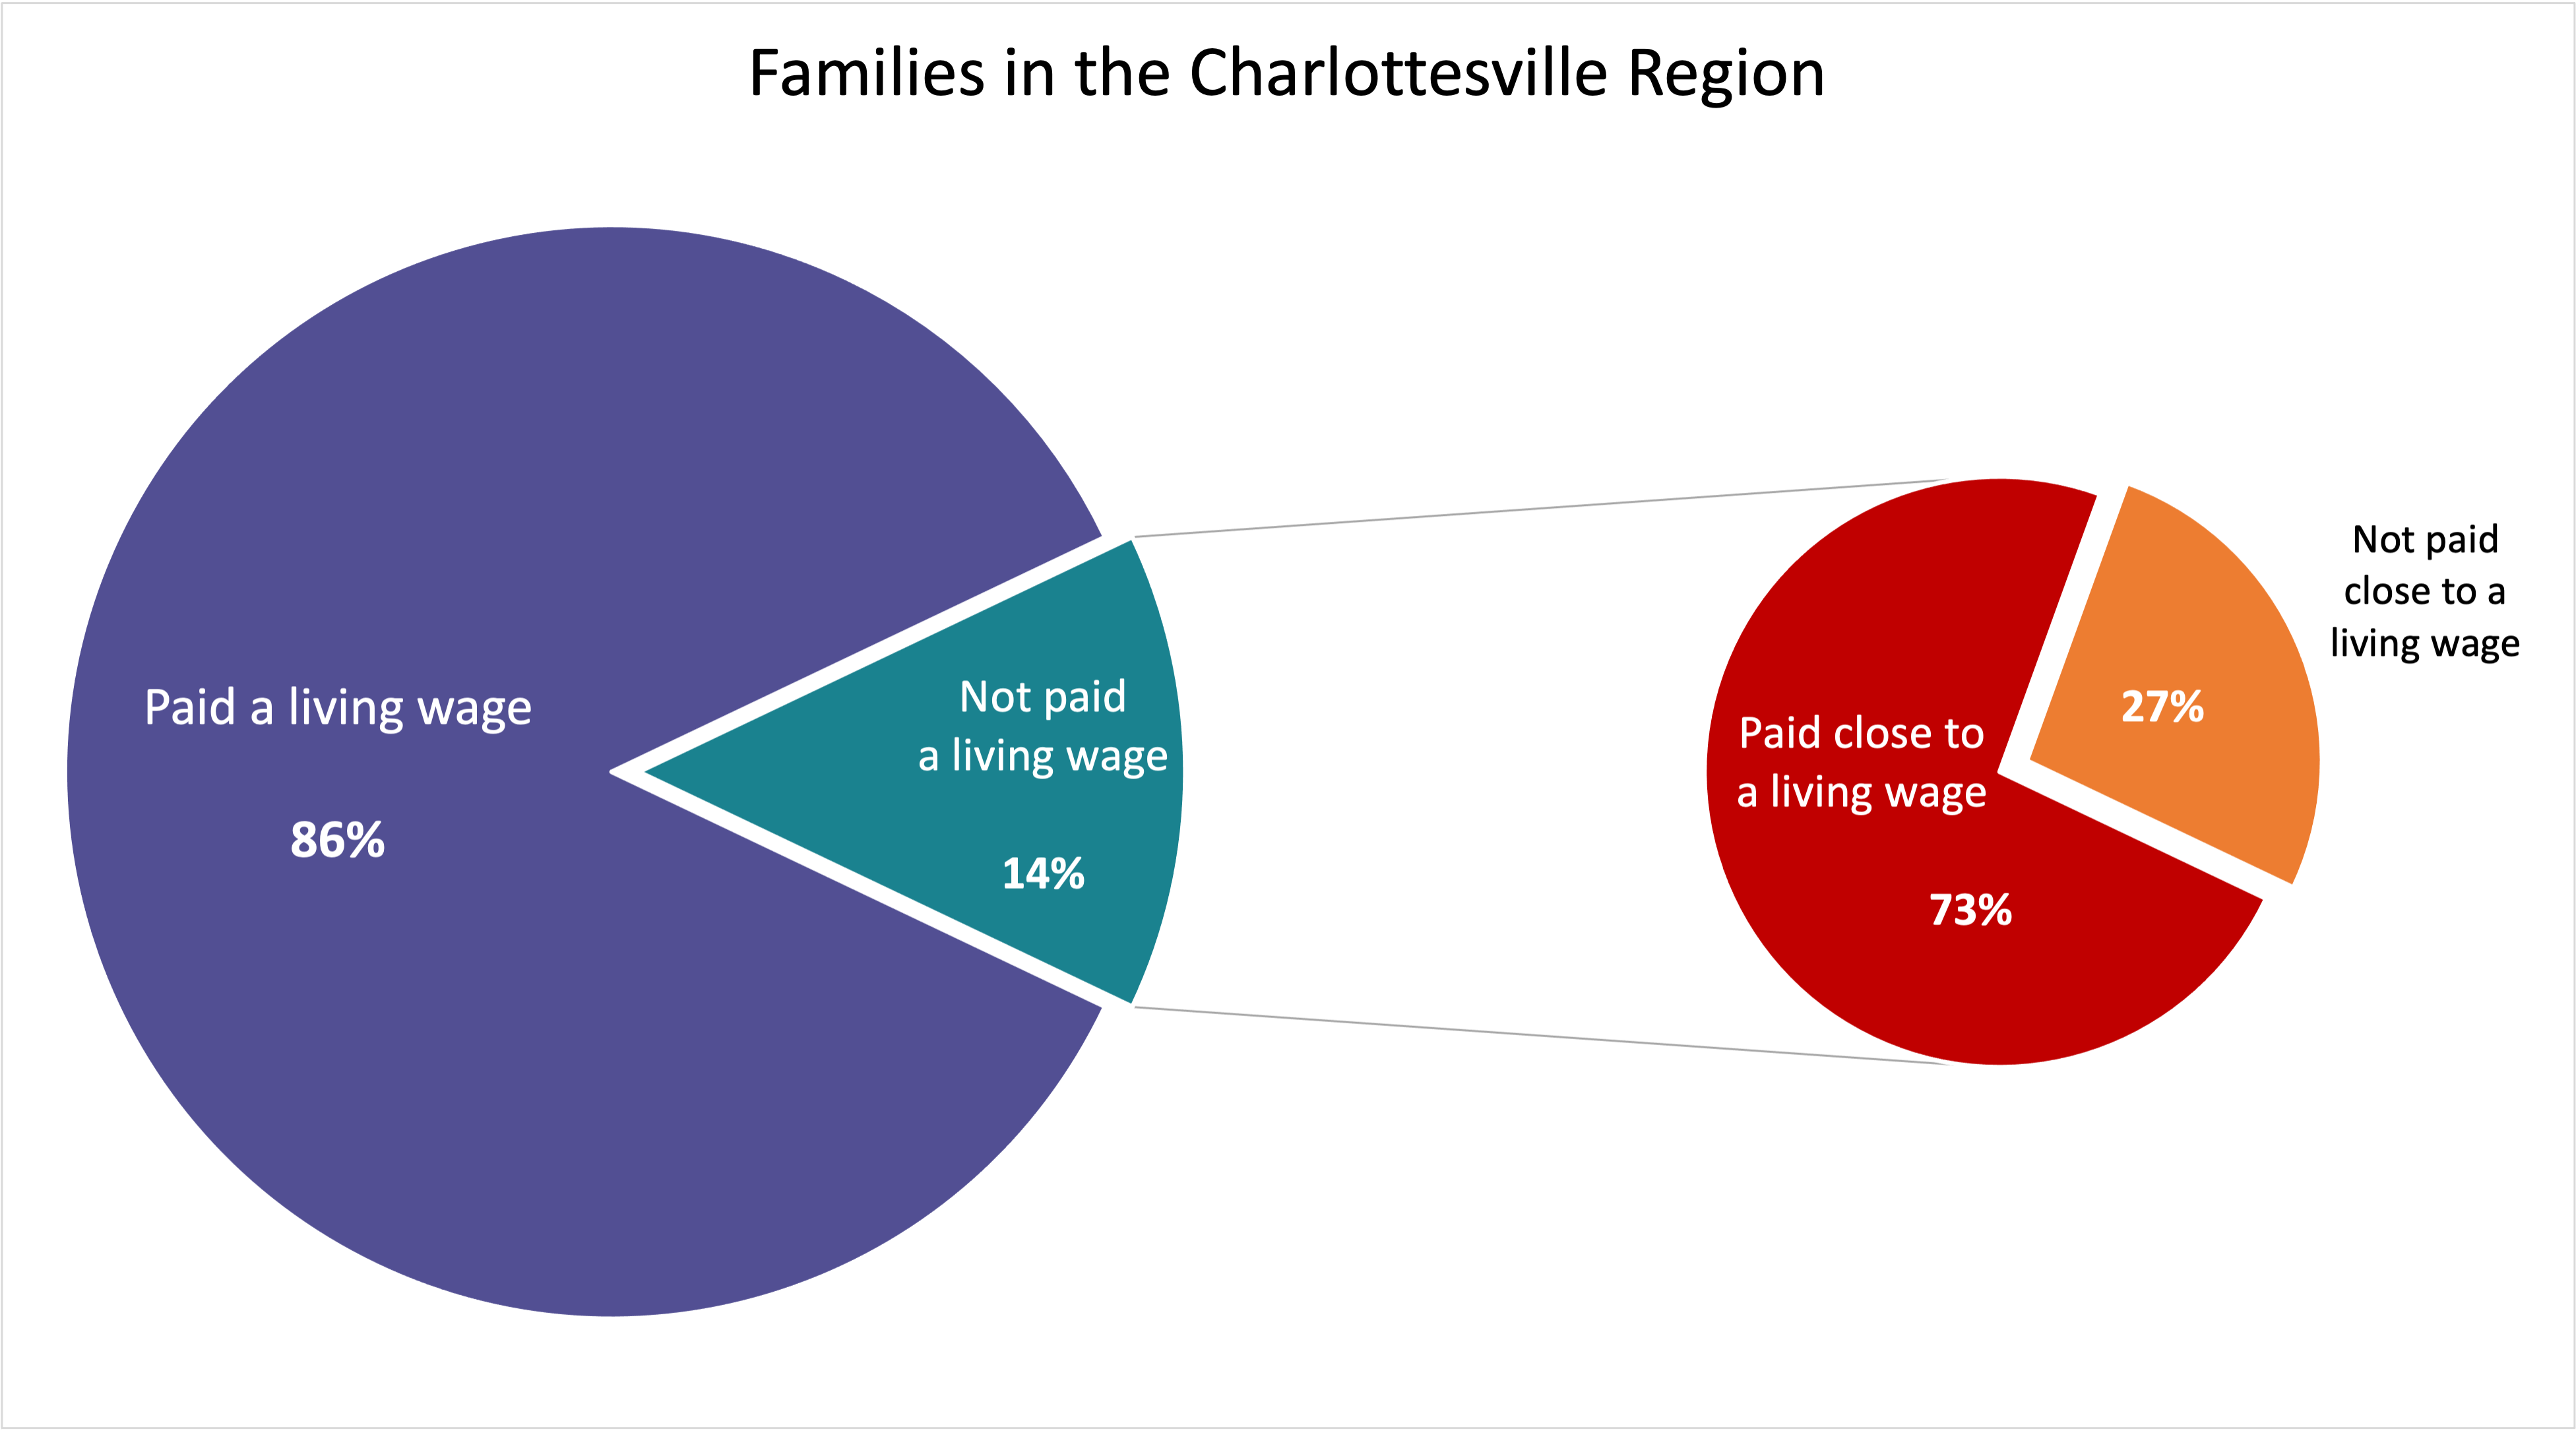
\includegraphics[width=1\linewidth]{images/PictureChart} \end{center}

To get ahead, those workers will need jobs and careers that pay enough
to support their families.

We all benefit when the families in our community have access to jobs
that pay sufficient incomes. Among the many advantages include:

\textbf{Children do better.} Graduating from college continues to be the
fastest route to economic security, yet economic insecurity limits
access to higher education. As Robert Putnam's work shows, ``a family's
socioeconomic status {[}has{]} become even more important than test
scores in predicting which eighth graders would graduate from college.
High-scoring poor kids are now slightly less likely (29\%) to get a
college degree than low-scoring rich kids (30\%).''\footnote{Putnam, R.
  (2015). Our Kids: The American Dream in Crisis. New York, NY: Simon \&
  Schuster, 189-190.}

\textbf{Local businesses benefit.} Employees are also consumers, and
increased income among a region's workers means more spending power,
which is better for the economy, especially the local economy.

\textbf{Taxpayers benefit.} Given the chance, families want to provide
for themselves. When they are able to do so, they require less support
from others.

\textbf{People live longer.} According to the Centers for Disease
Control, the biggest contributor to poor health is low socio-economic
status. The Health Inequality Project estimates that a woman in the
Charlottesville area in the lowest income quartile has a life expectancy
of seven years less than a woman from the highest income quartile; among
men in our region, the life expectancy gap is nearly ten
years.\footnote{Chetty R., Stepner M., Abraham S., Lin S., Scuderi B.,
  Turner N., Bergeron A., and Cutler D., (2016). The Association Between
  Income and Life Expectancy in the United States, 2001-2014. JAMA
  315:1750--1766. \url{doi:10.1001/jama.2016.4226}. Data:
  \url{https://healthinequality.org/data/}}

\textbf{The community thrives.} A community thrives when its residents
thrive. Residents thrive when their capacity as human beings is
unleashed. And their capacity as human beings can only be unleashed when
their basic needs are met.

\hypertarget{the-intersection-with-race}{%
\subsection{The Intersection with
Race}\label{the-intersection-with-race}}

Too many families are struggling in our region, but these burdens are
not equally shared. Throughout our country and our history, the labor of
our Black neighbors has been systematically valued less than the labor
of our White neighbors. The undervaluing of Black labor has been
reinforced through many policies from those we've collectively
recognized as racially discriminatory---enslavement, Black codes, Jim
Crow, Massive Resistance---to ongoing and often unacknowledged
choices---a legacy of disinvestment in and displacement of Black
communities, the blocking of wealth creation through red-lining and
predatory lending, disproportionate contact with law enforcement and
overincarceration, disenfranchisement and political demobilization,
overt and subconscious negative stereotypes. And the list could go on.

These policies and choices have generated a significant racial wealth
gap. The Federal Reserve Bank of St.~Louis calculated that the average
net worth of a white family in America was ten times greater than the
net worth of a Black family, as shown below.\footnote{Mock, B. (2019,
  March 21). Why Can't We Close the Racial Wealth Gap? Bloomberg City
  Lab. Retrieved from
  \url{https://www.bloomberg.com/news/articles/2019-03-21/how-income-inequality-feeds-the-racial-wealth-gap}.
  Data on unequal labor income in our region comes from U.S. Census
  Bureau (2020). Family Income in the Past 12 Months. American Community
  Survey 5-Year Estimates, 2014-2018, Tables B19101, 19101A, 19101B.}

\begin{center}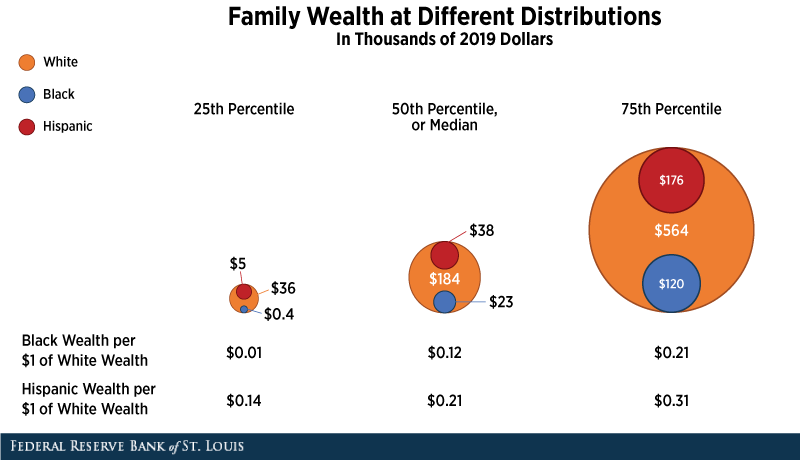
\includegraphics[width=0.8\linewidth]{images/WealthGap} \end{center}

That racial wealth gap is best explained by unequal labor income,
according to research from the Federal Reserve Bank of
Cleveland.\footnote{Mock, B. (2019, March 21). Why Can't We Close the
  Racial Wealth Gap? Bloomberg City Lab. Retrieved from
  \url{https://www.bloomberg.com/news/articles/2019-03-21/how-income-inequality-feeds-the-racial-wealth-gap}.}

\begin{center}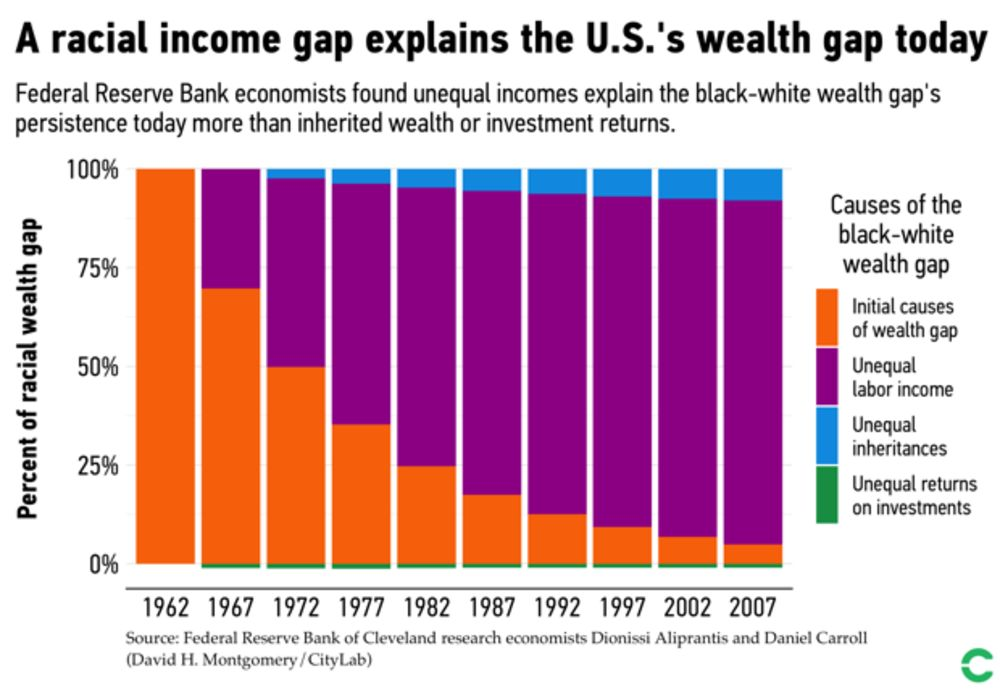
\includegraphics[width=0.8\linewidth]{images/IncomeGap} \end{center}

This struggle is not new. When Dr.~Martin Luther King, Jr.~stood on the
steps of the Lincoln Memorial on August 28, 1963 to deliver his iconic I
Have A Dream speech, he was addressing a ``March for Jobs and Freedom.''
When he was assassinated at the Lorraine Motel on April 4, 1968, he was
in Memphis to stand shoulder to shoulder with Black sanitation workers
fighting for higher wages.

This struggle is also local, as was made stark in the violence and
terror of August 11 and 12, 2017. And the unequal labor income within
the nation is reflected in our community as well. As shown below, the
percent of Black families making less than family-sustaining income is
consistently higher across our region than the percent of white families
struggling, and is especially high in Albemarle and
Charlottesville.\footnote{Data on unequal labor income in our region
  comes from U.S. Census Bureau (2020). Family Income in the Past 12
  Months. American Community Survey 5-Year Estimates, 2014-2018, Tables
  B19101, 19101A, 19101B.}

\hypertarget{families-making-under-35000-by-race}{%
\subsubsection{Families Making under \$35,000 by
Race}\label{families-making-under-35000-by-race}}

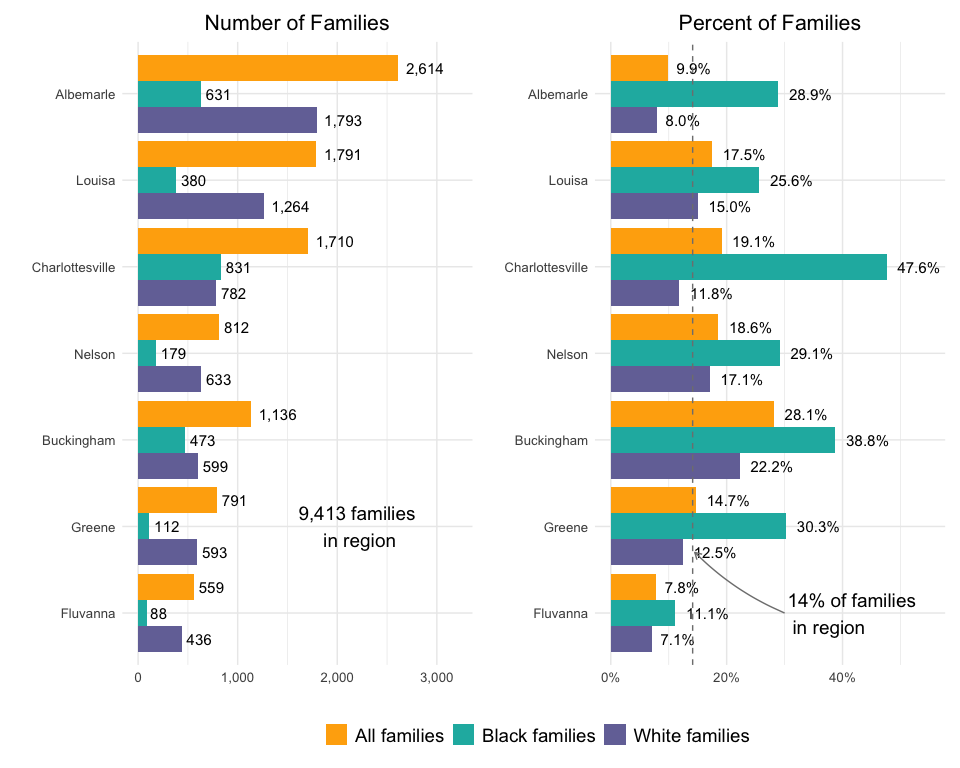
\includegraphics{orange-dot-test_files/figure-latex/unnamed-chunk-6-1.pdf}

We need to be intentional about helping all families in our community
who are struggling to achieve self-sufficient income, but must be
especially attentive to Black families who are struggling in our economy
as they may understandably be distrustful or disconnected from the very
institutions positioned to help.

\hypertarget{locality-profiles}{%
\subsection{Locality Profiles}\label{locality-profiles}}

The following sections explore each locality separately, detailing what
it costs to be self-sufficient in each of the localities that comprise
the region---including the costs of food\footnote{U.S. Department of
  Agriculture, Center for Nutrition Policy and Promotion (2022).
  Official USDA Food Plans: Cost of Food at Home at Four Levels, U.S.
  Average, May 2022, Weekly Cost of the Low-Cost Plan. Retrieved from
  \url{https://www.fns.usda.gov/sites/default/files/media/file/CostofFoodMay2022Thrifty.pdf}},
shelter\footnote{Virginia Housing (2022). 2022 Fair Market Rents.
  Retrieved from
  \url{https://www.huduser.gov/portal/datasets/fmr/fmrs/FY2022_code/2022summary.odn}},
clothing\footnote{U.S. Department of Agriculture, Center for Nutrition
  Policy and Promotion (2017). Expenditures on Children by Families,
  Estimated annual expenditures on a child by single-parent families.
  Retrieved from
  \url{https://www.fns.usda.gov/sites/default/files/resource-files/crc2015-march2017.pdf}
  and U.S. Bureau of Labor Statistics (2020). Consumer Expenditures
  Survey, CE Tables, Age of Reference Person, Apparel and Services by
  Women, 16 and over. Retrieved from
  \url{https://www.bls.gov/cex/tables/calendar-year/mean-item-share-average-standard-error/reference-person-age-ranges-2020.pdf}},
utilities\footnote{Virginia Housing Development Authority (2022).
  Allowances for Tenant-Furnished Utilities and Other Services, Two
  Exposed UA Schedule. Retrieved from
  \url{https://mc-0e9acafd-48f4-4c49-b478-6257-cdn-endpoint.azureedge.net/-/media/docs/partners/housing-choice-vouchers/utility-allowance/2exposed-walls.pdf?rev=91c81573c2e94b8cb314f871bbad5e65\&hash=666946C107D54311AC4222AC1E81F850}
  and the U.S. Bureau of Labor Statistics (2020), Consumer Expenditure
  Survey, Telephone Services. Retrieved from
  \url{https://www.bls.gov/cex/tables/calendar-year/mean-item-share-average-standard-error/reference-person-age-ranges-2020.pdf}},
childcare\footnote{Virginia Department of Social Services, Division of
  Child Care and Early Childhood Development (2021). Child Care Subsidy
  Program Guidance Manual. Richmond, Virginia. Retrieved from
  \url{https://doe.virginia.gov/cc/files/child-care-subsidy-guidance-manual.pdf}.},
transportation\footnote{U.S. Bureau of Labor Statistics (2020). Consumer
  Expenditures Survey, CE Tables, Age of Reference Person, Apparel and
  Services by Women, 16 and over. Retrieved from
  \url{https://www.bls.gov/cex/tables/calendar-year/mean-item-share-average-standard-error/reference-person-age-ranges-2020.pdf}},
and necessary costs\footnote{Garner, T. (2010). Supplemental Poverty
  Measure Thresholds: Laying the Foundation. Washington DC: Bureau of
  Labor Statistics.}---and describing how many families in each locality
are struggling.

We show, too, how families are faring by race, as above, and by place.
Places, or the neighborhoods within localities, are captured with census
tracts, areas used by the United States Census Bureau to approximate
neighborhoods. Census tracts are roughly equal in population and are
bounded by major roads, rivers and railroad tracks. The geographic
variation in our region is evident across these census tracts.
Charlottesville for example, is a city of roughly 10 square miles that
are more densely populated. Albemarle surrounds Charlottesville and
dwarfs it physically at 726 square miles, but it has both dense
neighborhoods and sprawling rural ones. While there is variation across
the communities that define the greater Charlottesville region, there is
one constant: throughout the region there are hundreds of families who
struggle every day to put a roof over their heads, food in their
bellies, clothes on their backs and heat in their homes.

\hypertarget{localities}{%
\subsubsection{Localities}\label{localities}}

\hypertarget{albemarle-county}{%
\paragraph{Albemarle County}\label{albemarle-county}}

\hypertarget{albemarle-county-1}{%
\subparagraph{Albemarle County}\label{albemarle-county-1}}

There are 26,522 families living in Albemarle County. Of these, 2,614
(9.9\%) do not earn enough to provide for their basic needs and the
costs associated with working.

Albemarle County at a glance:

\begin{itemize}
\item
  Albemarle and Charlottesville are the most expensive localities in the
  region given the costs of housing and childcare.
\item
  Albemarle, relative to the other localities, has the highest number of
  families making \$25,000-34,999 a year, just below the minimum target
  threshold.
\item
  Albemarle has one of the largest racial disparities among struggling
  families; the percent of Black families making under \$35,000 (29\%)
  is 21\% higher than the percent of white families making under
  \$35,000 (8\%).
\item
  Families making less than \$35,000 tend to be more highly concentrated
  near the University of Virginia and the Oak Hill neighborhood.
\end{itemize}

\hypertarget{expenses-single-householder-2-children-1-toddler}{%
\subparagraph{Expenses: Single Householder + 2 Children (1
Toddler)}\label{expenses-single-householder-2-children-1-toddler}}

\global\setlength{\Oldarrayrulewidth}{\arrayrulewidth}

\global\setlength{\Oldtabcolsep}{\tabcolsep}

\setlength{\tabcolsep}{0pt}

\renewcommand*{\arraystretch}{1.5}



\providecommand{\ascline}[3]{\noalign{\global\arrayrulewidth #1}\arrayrulecolor[HTML]{#2}\cline{#3}}

\begin{longtable}[c]{|p{5.00in}|p{5.00in}|p{5.00in}|p{5.00in}}



\hhline{>{\arrayrulecolor[HTML]{666666}\global\arrayrulewidth=2pt}->{\arrayrulecolor[HTML]{666666}\global\arrayrulewidth=2pt}->{\arrayrulecolor[HTML]{666666}\global\arrayrulewidth=2pt}->{\arrayrulecolor[HTML]{666666}\global\arrayrulewidth=2pt}-}

\multicolumn{1}{>{\cellcolor[HTML]{FFFFFF}\centering}p{\dimexpr 5in+0\tabcolsep}}{\textcolor[HTML]{000000}{\fontsize{11}{11}\selectfont{Expense}}} & \multicolumn{1}{>{\cellcolor[HTML]{FFFFFF}\centering}p{\dimexpr 5in+0\tabcolsep}}{\textcolor[HTML]{000000}{\fontsize{11}{11}\selectfont{Annual}}} & \multicolumn{1}{>{\cellcolor[HTML]{FFFFFF}\centering}p{\dimexpr 5in+0\tabcolsep}}{\textcolor[HTML]{000000}{\fontsize{11}{11}\selectfont{Monthly}}} & \multicolumn{1}{>{\cellcolor[HTML]{FFFFFF}\centering}p{\dimexpr 5in+0\tabcolsep}}{\textcolor[HTML]{000000}{\fontsize{11}{11}\selectfont{Weekly}}} \\

\noalign{\global\arrayrulewidth 0pt}\arrayrulecolor[HTML]{000000}

\hhline{>{\arrayrulecolor[HTML]{666666}\global\arrayrulewidth=2pt}->{\arrayrulecolor[HTML]{666666}\global\arrayrulewidth=2pt}->{\arrayrulecolor[HTML]{666666}\global\arrayrulewidth=2pt}->{\arrayrulecolor[HTML]{666666}\global\arrayrulewidth=2pt}-}\endhead



\multicolumn{1}{>{\cellcolor[HTML]{FFFFFF}\centering}p{\dimexpr 5in+0\tabcolsep}}{\textcolor[HTML]{000000}{\fontsize{11}{11}\selectfont{Food}}} & \multicolumn{1}{>{\cellcolor[HTML]{FFFFFF}\centering}p{\dimexpr 5in+0\tabcolsep}}{\textcolor[HTML]{000000}{\fontsize{11}{11}\selectfont{6,630.0}}} & \multicolumn{1}{>{\cellcolor[HTML]{FFFFFF}\centering}p{\dimexpr 5in+0\tabcolsep}}{\textcolor[HTML]{000000}{\fontsize{11}{11}\selectfont{552.50}}} & \multicolumn{1}{>{\cellcolor[HTML]{FFFFFF}\centering}p{\dimexpr 5in+0\tabcolsep}}{\textcolor[HTML]{000000}{\fontsize{11}{11}\selectfont{127.50}}} \\

\noalign{\global\arrayrulewidth 0pt}\arrayrulecolor[HTML]{000000}

\hhline{>{\arrayrulecolor[HTML]{BEBEBE}\global\arrayrulewidth=1pt}->{\arrayrulecolor[HTML]{BEBEBE}\global\arrayrulewidth=1pt}->{\arrayrulecolor[HTML]{BEBEBE}\global\arrayrulewidth=1pt}->{\arrayrulecolor[HTML]{BEBEBE}\global\arrayrulewidth=1pt}-}



\multicolumn{1}{>{\cellcolor[HTML]{FFFFFF}\centering}p{\dimexpr 5in+0\tabcolsep}}{\textcolor[HTML]{000000}{\fontsize{11}{11}\selectfont{Clothing}}} & \multicolumn{1}{>{\cellcolor[HTML]{FFFFFF}\centering}p{\dimexpr 5in+0\tabcolsep}}{\textcolor[HTML]{000000}{\fontsize{11}{11}\selectfont{2,334.0}}} & \multicolumn{1}{>{\cellcolor[HTML]{FFFFFF}\centering}p{\dimexpr 5in+0\tabcolsep}}{\textcolor[HTML]{000000}{\fontsize{11}{11}\selectfont{194.50}}} & \multicolumn{1}{>{\cellcolor[HTML]{FFFFFF}\centering}p{\dimexpr 5in+0\tabcolsep}}{\textcolor[HTML]{000000}{\fontsize{11}{11}\selectfont{44.88}}} \\

\noalign{\global\arrayrulewidth 0pt}\arrayrulecolor[HTML]{000000}

\hhline{>{\arrayrulecolor[HTML]{BEBEBE}\global\arrayrulewidth=1pt}->{\arrayrulecolor[HTML]{BEBEBE}\global\arrayrulewidth=1pt}->{\arrayrulecolor[HTML]{BEBEBE}\global\arrayrulewidth=1pt}->{\arrayrulecolor[HTML]{BEBEBE}\global\arrayrulewidth=1pt}-}



\multicolumn{1}{>{\cellcolor[HTML]{FFFFFF}\centering}p{\dimexpr 5in+0\tabcolsep}}{\textcolor[HTML]{000000}{\fontsize{11}{11}\selectfont{Shelter}}} & \multicolumn{1}{>{\cellcolor[HTML]{FFFFFF}\centering}p{\dimexpr 5in+0\tabcolsep}}{\textcolor[HTML]{000000}{\fontsize{11}{11}\selectfont{15,168.0}}} & \multicolumn{1}{>{\cellcolor[HTML]{FFFFFF}\centering}p{\dimexpr 5in+0\tabcolsep}}{\textcolor[HTML]{000000}{\fontsize{11}{11}\selectfont{1,264.00}}} & \multicolumn{1}{>{\cellcolor[HTML]{FFFFFF}\centering}p{\dimexpr 5in+0\tabcolsep}}{\textcolor[HTML]{000000}{\fontsize{11}{11}\selectfont{291.69}}} \\

\noalign{\global\arrayrulewidth 0pt}\arrayrulecolor[HTML]{000000}

\hhline{>{\arrayrulecolor[HTML]{BEBEBE}\global\arrayrulewidth=1pt}->{\arrayrulecolor[HTML]{BEBEBE}\global\arrayrulewidth=1pt}->{\arrayrulecolor[HTML]{BEBEBE}\global\arrayrulewidth=1pt}->{\arrayrulecolor[HTML]{BEBEBE}\global\arrayrulewidth=1pt}-}



\multicolumn{1}{>{\cellcolor[HTML]{FFFFFF}\centering}p{\dimexpr 5in+0\tabcolsep}}{\textcolor[HTML]{000000}{\fontsize{11}{11}\selectfont{Utilities}}} & \multicolumn{1}{>{\cellcolor[HTML]{FFFFFF}\centering}p{\dimexpr 5in+0\tabcolsep}}{\textcolor[HTML]{000000}{\fontsize{11}{11}\selectfont{3,325.0}}} & \multicolumn{1}{>{\cellcolor[HTML]{FFFFFF}\centering}p{\dimexpr 5in+0\tabcolsep}}{\textcolor[HTML]{000000}{\fontsize{11}{11}\selectfont{277.08}}} & \multicolumn{1}{>{\cellcolor[HTML]{FFFFFF}\centering}p{\dimexpr 5in+0\tabcolsep}}{\textcolor[HTML]{000000}{\fontsize{11}{11}\selectfont{63.94}}} \\

\noalign{\global\arrayrulewidth 0pt}\arrayrulecolor[HTML]{000000}

\hhline{>{\arrayrulecolor[HTML]{BEBEBE}\global\arrayrulewidth=1pt}->{\arrayrulecolor[HTML]{BEBEBE}\global\arrayrulewidth=1pt}->{\arrayrulecolor[HTML]{BEBEBE}\global\arrayrulewidth=1pt}->{\arrayrulecolor[HTML]{BEBEBE}\global\arrayrulewidth=1pt}-}



\multicolumn{1}{>{\cellcolor[HTML]{FFFFFF}\centering}p{\dimexpr 5in+0\tabcolsep}}{\textcolor[HTML]{000000}{\fontsize{11}{11}\selectfont{Necessary\ Costs}}} & \multicolumn{1}{>{\cellcolor[HTML]{FFFFFF}\centering}p{\dimexpr 5in+0\tabcolsep}}{\textcolor[HTML]{000000}{\fontsize{11}{11}\selectfont{5,491.4}}} & \multicolumn{1}{>{\cellcolor[HTML]{FFFFFF}\centering}p{\dimexpr 5in+0\tabcolsep}}{\textcolor[HTML]{000000}{\fontsize{11}{11}\selectfont{457.62}}} & \multicolumn{1}{>{\cellcolor[HTML]{FFFFFF}\centering}p{\dimexpr 5in+0\tabcolsep}}{\textcolor[HTML]{000000}{\fontsize{11}{11}\selectfont{105.60}}} \\

\noalign{\global\arrayrulewidth 0pt}\arrayrulecolor[HTML]{000000}

\hhline{>{\arrayrulecolor[HTML]{BEBEBE}\global\arrayrulewidth=1pt}->{\arrayrulecolor[HTML]{BEBEBE}\global\arrayrulewidth=1pt}->{\arrayrulecolor[HTML]{BEBEBE}\global\arrayrulewidth=1pt}->{\arrayrulecolor[HTML]{BEBEBE}\global\arrayrulewidth=1pt}-}



\multicolumn{1}{>{\cellcolor[HTML]{FFAD0A}\centering}p{\dimexpr 5in+0\tabcolsep}}{\textcolor[HTML]{000000}{\fontsize{11}{11}\selectfont{Survival\ Expenses}}} & \multicolumn{1}{>{\cellcolor[HTML]{FFAD0A}\centering}p{\dimexpr 5in+0\tabcolsep}}{\textcolor[HTML]{000000}{\fontsize{11}{11}\selectfont{32,948.4}}} & \multicolumn{1}{>{\cellcolor[HTML]{FFAD0A}\centering}p{\dimexpr 5in+0\tabcolsep}}{\textcolor[HTML]{000000}{\fontsize{11}{11}\selectfont{2,745.70}}} & \multicolumn{1}{>{\cellcolor[HTML]{FFAD0A}\centering}p{\dimexpr 5in+0\tabcolsep}}{\textcolor[HTML]{000000}{\fontsize{11}{11}\selectfont{633.62}}} \\

\noalign{\global\arrayrulewidth 0pt}\arrayrulecolor[HTML]{000000}

\hhline{>{\arrayrulecolor[HTML]{BEBEBE}\global\arrayrulewidth=1pt}->{\arrayrulecolor[HTML]{BEBEBE}\global\arrayrulewidth=1pt}->{\arrayrulecolor[HTML]{BEBEBE}\global\arrayrulewidth=1pt}->{\arrayrulecolor[HTML]{BEBEBE}\global\arrayrulewidth=1pt}-}



\multicolumn{1}{>{\cellcolor[HTML]{FFFFFF}\centering}p{\dimexpr 5in+0\tabcolsep}}{\textcolor[HTML]{000000}{\fontsize{11}{11}\selectfont{Childcare}}} & \multicolumn{1}{>{\cellcolor[HTML]{FFFFFF}\centering}p{\dimexpr 5in+0\tabcolsep}}{\textcolor[HTML]{000000}{\fontsize{11}{11}\selectfont{21,580.0}}} & \multicolumn{1}{>{\cellcolor[HTML]{FFFFFF}\centering}p{\dimexpr 5in+0\tabcolsep}}{\textcolor[HTML]{000000}{\fontsize{11}{11}\selectfont{1,798.00}}} & \multicolumn{1}{>{\cellcolor[HTML]{FFFFFF}\centering}p{\dimexpr 5in+0\tabcolsep}}{\textcolor[HTML]{000000}{\fontsize{11}{11}\selectfont{415.00}}} \\

\noalign{\global\arrayrulewidth 0pt}\arrayrulecolor[HTML]{000000}

\hhline{>{\arrayrulecolor[HTML]{BEBEBE}\global\arrayrulewidth=1pt}->{\arrayrulecolor[HTML]{BEBEBE}\global\arrayrulewidth=1pt}->{\arrayrulecolor[HTML]{BEBEBE}\global\arrayrulewidth=1pt}->{\arrayrulecolor[HTML]{BEBEBE}\global\arrayrulewidth=1pt}-}



\multicolumn{1}{>{\cellcolor[HTML]{FFFFFF}\centering}p{\dimexpr 5in+0\tabcolsep}}{\textcolor[HTML]{000000}{\fontsize{11}{11}\selectfont{Transportation}}} & \multicolumn{1}{>{\cellcolor[HTML]{FFFFFF}\centering}p{\dimexpr 5in+0\tabcolsep}}{\textcolor[HTML]{000000}{\fontsize{11}{11}\selectfont{3,996.0}}} & \multicolumn{1}{>{\cellcolor[HTML]{FFFFFF}\centering}p{\dimexpr 5in+0\tabcolsep}}{\textcolor[HTML]{000000}{\fontsize{11}{11}\selectfont{333.00}}} & \multicolumn{1}{>{\cellcolor[HTML]{FFFFFF}\centering}p{\dimexpr 5in+0\tabcolsep}}{\textcolor[HTML]{000000}{\fontsize{11}{11}\selectfont{76.85}}} \\

\noalign{\global\arrayrulewidth 0pt}\arrayrulecolor[HTML]{000000}

\hhline{>{\arrayrulecolor[HTML]{BEBEBE}\global\arrayrulewidth=1pt}->{\arrayrulecolor[HTML]{BEBEBE}\global\arrayrulewidth=1pt}->{\arrayrulecolor[HTML]{BEBEBE}\global\arrayrulewidth=1pt}->{\arrayrulecolor[HTML]{BEBEBE}\global\arrayrulewidth=1pt}-}



\multicolumn{1}{>{\cellcolor[HTML]{EE6100}\centering}p{\dimexpr 5in+0\tabcolsep}}{\textcolor[HTML]{FFFFFF}{\fontsize{11}{11}\selectfont{Total\ Expenses}}} & \multicolumn{1}{>{\cellcolor[HTML]{EE6100}\centering}p{\dimexpr 5in+0\tabcolsep}}{\textcolor[HTML]{FFFFFF}{\fontsize{11}{11}\selectfont{58,524.4}}} & \multicolumn{1}{>{\cellcolor[HTML]{EE6100}\centering}p{\dimexpr 5in+0\tabcolsep}}{\textcolor[HTML]{FFFFFF}{\fontsize{11}{11}\selectfont{4,116.20}}} & \multicolumn{1}{>{\cellcolor[HTML]{EE6100}\centering}p{\dimexpr 5in+0\tabcolsep}}{\textcolor[HTML]{FFFFFF}{\fontsize{11}{11}\selectfont{949.89}}} \\

\noalign{\global\arrayrulewidth 0pt}\arrayrulecolor[HTML]{000000}

\hhline{>{\arrayrulecolor[HTML]{666666}\global\arrayrulewidth=2pt}->{\arrayrulecolor[HTML]{666666}\global\arrayrulewidth=2pt}->{\arrayrulecolor[HTML]{666666}\global\arrayrulewidth=2pt}->{\arrayrulecolor[HTML]{666666}\global\arrayrulewidth=2pt}-}



\end{longtable}



\arrayrulecolor[HTML]{000000}

\global\setlength{\arrayrulewidth}{\Oldarrayrulewidth}

\global\setlength{\tabcolsep}{\Oldtabcolsep}

\renewcommand*{\arraystretch}{1}

\hypertarget{breakdown-of-families-making-under-35000-in-albemarle-county}{%
\subparagraph{Breakdown of Families Making under \$35,000 in Albemarle
County}\label{breakdown-of-families-making-under-35000-in-albemarle-county}}

\global\setlength{\Oldarrayrulewidth}{\arrayrulewidth}

\global\setlength{\Oldtabcolsep}{\tabcolsep}

\setlength{\tabcolsep}{0pt}

\renewcommand*{\arraystretch}{1.5}



\providecommand{\ascline}[3]{\noalign{\global\arrayrulewidth #1}\arrayrulecolor[HTML]{#2}\cline{#3}}

\begin{longtable}[c]{|p{5.00in}|p{5.00in}|p{5.00in}|p{5.00in}}



\hhline{>{\arrayrulecolor[HTML]{666666}\global\arrayrulewidth=2pt}->{\arrayrulecolor[HTML]{666666}\global\arrayrulewidth=2pt}->{\arrayrulecolor[HTML]{666666}\global\arrayrulewidth=2pt}->{\arrayrulecolor[HTML]{666666}\global\arrayrulewidth=2pt}-}

\multicolumn{1}{>{\cellcolor[HTML]{FFFFFF}\centering}p{\dimexpr 5in+0\tabcolsep}}{\textcolor[HTML]{000000}{\fontsize{11}{11}\selectfont{Income}}} & \multicolumn{1}{>{\cellcolor[HTML]{FFFFFF}\centering}p{\dimexpr 5in+0\tabcolsep}}{\textcolor[HTML]{000000}{\fontsize{11}{11}\selectfont{Number}}} & \multicolumn{1}{>{\cellcolor[HTML]{FFFFFF}\centering}p{\dimexpr 5in+0\tabcolsep}}{\textcolor[HTML]{000000}{\fontsize{11}{11}\selectfont{Percent}}} & \multicolumn{1}{>{\cellcolor[HTML]{FFFFFF}\centering}p{\dimexpr 5in+0\tabcolsep}}{\textcolor[HTML]{000000}{\fontsize{11}{11}\selectfont{Cumulative}}} \\

\noalign{\global\arrayrulewidth 0pt}\arrayrulecolor[HTML]{000000}

\hhline{>{\arrayrulecolor[HTML]{666666}\global\arrayrulewidth=2pt}->{\arrayrulecolor[HTML]{666666}\global\arrayrulewidth=2pt}->{\arrayrulecolor[HTML]{666666}\global\arrayrulewidth=2pt}->{\arrayrulecolor[HTML]{666666}\global\arrayrulewidth=2pt}-}\endhead



\multicolumn{1}{>{\cellcolor[HTML]{FFFFFF}\centering}p{\dimexpr 5in+0\tabcolsep}}{\textcolor[HTML]{000000}{\fontsize{11}{11}\selectfont{\$0\ -\ \$9,999}}} & \multicolumn{1}{>{\cellcolor[HTML]{FFFFFF}\centering}p{\dimexpr 5in+0\tabcolsep}}{\textcolor[HTML]{000000}{\fontsize{11}{11}\selectfont{402}}} & \multicolumn{1}{>{\cellcolor[HTML]{FFFFFF}\centering}p{\dimexpr 5in+0\tabcolsep}}{\textcolor[HTML]{000000}{\fontsize{11}{11}\selectfont{15\%}}} & \multicolumn{1}{>{\cellcolor[HTML]{FFAD0A}\centering}p{\dimexpr 5in+0\tabcolsep}}{} \\

\noalign{\global\arrayrulewidth 0pt}\arrayrulecolor[HTML]{000000}

\hhline{>{\arrayrulecolor[HTML]{BEBEBE}\global\arrayrulewidth=1pt}->{\arrayrulecolor[HTML]{BEBEBE}\global\arrayrulewidth=1pt}->{\arrayrulecolor[HTML]{BEBEBE}\global\arrayrulewidth=1pt}->{\arrayrulecolor[HTML]{FFAD0A}\global\arrayrulewidth=1pt}-}



\multicolumn{1}{>{\cellcolor[HTML]{FFFFFF}\centering}p{\dimexpr 5in+0\tabcolsep}}{\textcolor[HTML]{000000}{\fontsize{11}{11}\selectfont{\$10,000\ -\ \$14,999}}} & \multicolumn{1}{>{\cellcolor[HTML]{FFFFFF}\centering}p{\dimexpr 5in+0\tabcolsep}}{\textcolor[HTML]{000000}{\fontsize{11}{11}\selectfont{178}}} & \multicolumn{1}{>{\cellcolor[HTML]{FFFFFF}\centering}p{\dimexpr 5in+0\tabcolsep}}{\textcolor[HTML]{000000}{\fontsize{11}{11}\selectfont{7\%}}} & \multicolumn{1}{>{\cellcolor[HTML]{FFAD0A}\centering}p{\dimexpr 5in+0\tabcolsep}}{\multirow[c]{-2}{*}{\parbox{5in}{\textcolor[HTML]{000000}{\fontsize{11}{11}\selectfont{22\%}}}}} \\

\noalign{\global\arrayrulewidth 0pt}\arrayrulecolor[HTML]{000000}

\hhline{>{\arrayrulecolor[HTML]{BEBEBE}\global\arrayrulewidth=1pt}->{\arrayrulecolor[HTML]{BEBEBE}\global\arrayrulewidth=1pt}->{\arrayrulecolor[HTML]{BEBEBE}\global\arrayrulewidth=1pt}->{\arrayrulecolor[HTML]{BEBEBE}\global\arrayrulewidth=1pt}-}



\multicolumn{1}{>{\cellcolor[HTML]{FFFFFF}\centering}p{\dimexpr 5in+0\tabcolsep}}{\textcolor[HTML]{000000}{\fontsize{11}{11}\selectfont{\$15,000\ -\ \$24,999}}} & \multicolumn{1}{>{\cellcolor[HTML]{FFFFFF}\centering}p{\dimexpr 5in+0\tabcolsep}}{\textcolor[HTML]{000000}{\fontsize{11}{11}\selectfont{641}}} & \multicolumn{1}{>{\cellcolor[HTML]{FFFFFF}\centering}p{\dimexpr 5in+0\tabcolsep}}{\textcolor[HTML]{000000}{\fontsize{11}{11}\selectfont{25\%}}} & \multicolumn{1}{>{\cellcolor[HTML]{EE6100}\centering}p{\dimexpr 5in+0\tabcolsep}}{} \\

\noalign{\global\arrayrulewidth 0pt}\arrayrulecolor[HTML]{000000}

\hhline{>{\arrayrulecolor[HTML]{BEBEBE}\global\arrayrulewidth=1pt}->{\arrayrulecolor[HTML]{BEBEBE}\global\arrayrulewidth=1pt}->{\arrayrulecolor[HTML]{BEBEBE}\global\arrayrulewidth=1pt}->{\arrayrulecolor[HTML]{EE6100}\global\arrayrulewidth=1pt}-}



\multicolumn{1}{>{\cellcolor[HTML]{FFFFFF}\centering}p{\dimexpr 5in+0\tabcolsep}}{\textcolor[HTML]{000000}{\fontsize{11}{11}\selectfont{\$25,000\ -\ \$34,999}}} & \multicolumn{1}{>{\cellcolor[HTML]{FFFFFF}\centering}p{\dimexpr 5in+0\tabcolsep}}{\textcolor[HTML]{000000}{\fontsize{11}{11}\selectfont{1,393}}} & \multicolumn{1}{>{\cellcolor[HTML]{FFFFFF}\centering}p{\dimexpr 5in+0\tabcolsep}}{\textcolor[HTML]{000000}{\fontsize{11}{11}\selectfont{53\%}}} & \multicolumn{1}{>{\cellcolor[HTML]{EE6100}\centering}p{\dimexpr 5in+0\tabcolsep}}{\multirow[c]{-2}{*}{\parbox{5in}{\textcolor[HTML]{FFFFFF}{\fontsize{11}{11}\selectfont{78\%}}}}} \\

\noalign{\global\arrayrulewidth 0pt}\arrayrulecolor[HTML]{000000}

\hhline{>{\arrayrulecolor[HTML]{BEBEBE}\global\arrayrulewidth=1pt}->{\arrayrulecolor[HTML]{BEBEBE}\global\arrayrulewidth=1pt}->{\arrayrulecolor[HTML]{BEBEBE}\global\arrayrulewidth=1pt}->{\arrayrulecolor[HTML]{BEBEBE}\global\arrayrulewidth=1pt}-}



\multicolumn{1}{>{\cellcolor[HTML]{FFFFFF}\centering}p{\dimexpr 5in+0\tabcolsep}}{\textcolor[HTML]{000000}{\fontsize{11}{11}\selectfont{Total}}} & \multicolumn{1}{>{\cellcolor[HTML]{FFFFFF}\centering}p{\dimexpr 5in+0\tabcolsep}}{\textcolor[HTML]{000000}{\fontsize{11}{11}\selectfont{2,614}}} & \multicolumn{2}{>{\cellcolor[HTML]{FFFFFF}\centering}p{\dimexpr 10in+2\tabcolsep}}{\textcolor[HTML]{000000}{\fontsize{11}{11}\selectfont{100\%}}} \\

\noalign{\global\arrayrulewidth 0pt}\arrayrulecolor[HTML]{000000}

\hhline{>{\arrayrulecolor[HTML]{666666}\global\arrayrulewidth=2pt}->{\arrayrulecolor[HTML]{666666}\global\arrayrulewidth=2pt}->{\arrayrulecolor[HTML]{666666}\global\arrayrulewidth=2pt}->{\arrayrulecolor[HTML]{666666}\global\arrayrulewidth=2pt}-}



\end{longtable}



\arrayrulecolor[HTML]{000000}

\global\setlength{\arrayrulewidth}{\Oldarrayrulewidth}

\global\setlength{\tabcolsep}{\Oldtabcolsep}

\renewcommand*{\arraystretch}{1}

As this table shows, 78\% of the families who cannot meet their basic
needs earn between \$15,000-\$35,000 annually. This strongly suggests
they are working, but not earning the wages or not getting the hours
they need to support their families.

The figure below shows the distribution of families in various pay
ranges, disaggregated by race. In a world with racial equity in income,
the bars for all families would be equal in height. In Albemarle, Black
families are over-represented at the low end of the pay ranges (under
\$35,000 a year) and under-represented at the high end of the pay ranges
(over \$100,000 a year). In other words, relative to white families,
Black families are more likely to be paid insufficient wages and less
likely to be high-earning.

Relative to the other localities, a higher share of Albemarle County
families fall into the high-earning pay ranges---this distribution is
likely related to the high cost of housing within the county.

\hypertarget{income-distribution-of-black-and-white-families-in-albemarle-county}{%
\subparagraph{Income Distribution of Black and White Families in
Albemarle
County}\label{income-distribution-of-black-and-white-families-in-albemarle-county}}

\begin{center}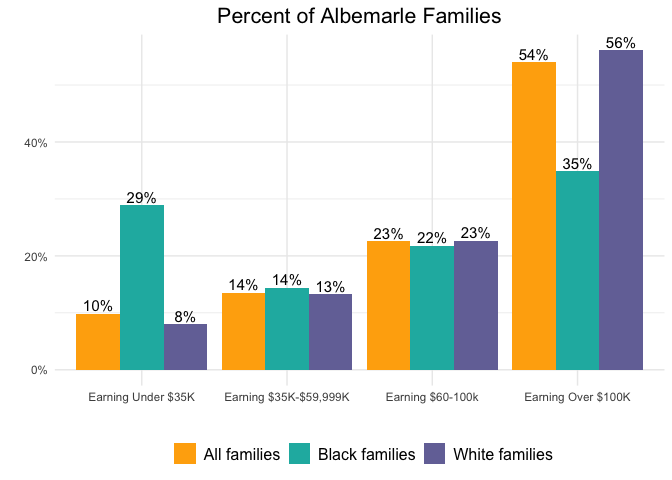
\includegraphics{orange-dot-test_files/figure-latex/unnamed-chunk-10-1} \end{center}

The maps below show the spatial relationship between income and
neighborhood. The color of each census tract in the county is based on
the median family income\footnote{The median family income is the value
  for which half of families in the area make less and half of the
  families in the area make more.} (the first map) or the percent of
families within the tract who make less than \$35,000 a year (the second
map). The maps show how residents are often concentrated into
neighborhoods with either high-earning or low-earning families, with
implications for the resources and opportunities available to the
families living within each tract.

To see which neighborhoods in Albemarle County have the highest and
lowest median family incomes, click on each tract to see its median
income and neighborhood names.

\hypertarget{median-family-income-in-albemarle-county}{%
\subparagraph{Median Family Income in Albemarle
County}\label{median-family-income-in-albemarle-county}}

The Carr's Hill-McCormick Road (UVA) tract has the lowest median family
incomes at \$53,047. While undergraduate students are largely excluded
from this analysis, as they aren't residing in family households, it may
include graduate students who are older, more likely to have families,
and more likely to live near the university alongside other low-paid
families. By contrast, the Ivy tract has the highest median family
income at \$190,353.

The following map shows the concentration of low-paid families. In
Albemarle County, again, the highest percentage of low-paid families are
concentrated in the Carr's Hill-McCormick Road (UVA), Oak Hill, and
Southwood tracts. Most of the other tracts in the county have no more
than 20\% of families making less than \$35,000 a year.

\hypertarget{percent-of-families-making-under-35000-in-albemarle-county}{%
\subparagraph{Percent of Families Making under \$35,000 in Albemarle
County}\label{percent-of-families-making-under-35000-in-albemarle-county}}

\protect\hyperlink{localities}{Return to Localities ↩︎}

\hypertarget{buckingham-county}{%
\paragraph{Buckingham County}\label{buckingham-county}}

\hypertarget{buckingham-county-1}{%
\subparagraph{Buckingham County}\label{buckingham-county-1}}

There are 4,037 families living in Buckingham County. This is the fewest
number of families in a locality in the region. Of these, 1,136 (28.1\%)
do not earn enough to provide for their basic needs and the costs
associated with working. This is the highest percent of families
struggling in localities across the region.

Buckingham County at a glance:

\begin{itemize}
\item
  Buckingham is the least expensive locality in the region for families
  given the cost of housing and childcare, but it has the largest
  percentage of families earning less than they need to afford basic
  needs.
\item
  In Buckingham, the percent of Black families making under \$35,000 a
  year (39\%) is 17\% higher than the percent of white families making
  under \$35,000 (22\%).
\item
  Buckingham, relative to the other localities, has the lowest percent
  of families making over \$100k/year---a higher share of Buckingham's
  families are concentrated in the lower pay ranges.
\item
  The concentration of low-paid families is less obvious in Buckingham
  relative to the other localities. Because so many families are paid
  under \$35,000 a year in Buckingham, the share of low-paid families is
  over 20\% across all tracts.
\end{itemize}

\hypertarget{expenses-single-householder-2-children-1-toddler-1}{%
\subparagraph{Expenses: Single Householder + 2 Children (1
Toddler)}\label{expenses-single-householder-2-children-1-toddler-1}}

\global\setlength{\Oldarrayrulewidth}{\arrayrulewidth}

\global\setlength{\Oldtabcolsep}{\tabcolsep}

\setlength{\tabcolsep}{0pt}

\renewcommand*{\arraystretch}{1.5}



\providecommand{\ascline}[3]{\noalign{\global\arrayrulewidth #1}\arrayrulecolor[HTML]{#2}\cline{#3}}

\begin{longtable}[c]{|p{5.00in}|p{5.00in}|p{5.00in}|p{5.00in}}



\hhline{>{\arrayrulecolor[HTML]{666666}\global\arrayrulewidth=2pt}->{\arrayrulecolor[HTML]{666666}\global\arrayrulewidth=2pt}->{\arrayrulecolor[HTML]{666666}\global\arrayrulewidth=2pt}->{\arrayrulecolor[HTML]{666666}\global\arrayrulewidth=2pt}-}

\multicolumn{1}{>{\cellcolor[HTML]{FFFFFF}\centering}p{\dimexpr 5in+0\tabcolsep}}{\textcolor[HTML]{000000}{\fontsize{11}{11}\selectfont{Expense}}} & \multicolumn{1}{>{\cellcolor[HTML]{FFFFFF}\centering}p{\dimexpr 5in+0\tabcolsep}}{\textcolor[HTML]{000000}{\fontsize{11}{11}\selectfont{Annual}}} & \multicolumn{1}{>{\cellcolor[HTML]{FFFFFF}\centering}p{\dimexpr 5in+0\tabcolsep}}{\textcolor[HTML]{000000}{\fontsize{11}{11}\selectfont{Monthly}}} & \multicolumn{1}{>{\cellcolor[HTML]{FFFFFF}\centering}p{\dimexpr 5in+0\tabcolsep}}{\textcolor[HTML]{000000}{\fontsize{11}{11}\selectfont{Weekly}}} \\

\noalign{\global\arrayrulewidth 0pt}\arrayrulecolor[HTML]{000000}

\hhline{>{\arrayrulecolor[HTML]{666666}\global\arrayrulewidth=2pt}->{\arrayrulecolor[HTML]{666666}\global\arrayrulewidth=2pt}->{\arrayrulecolor[HTML]{666666}\global\arrayrulewidth=2pt}->{\arrayrulecolor[HTML]{666666}\global\arrayrulewidth=2pt}-}\endhead



\multicolumn{1}{>{\cellcolor[HTML]{FFFFFF}\centering}p{\dimexpr 5in+0\tabcolsep}}{\textcolor[HTML]{000000}{\fontsize{11}{11}\selectfont{Food}}} & \multicolumn{1}{>{\cellcolor[HTML]{FFFFFF}\centering}p{\dimexpr 5in+0\tabcolsep}}{\textcolor[HTML]{000000}{\fontsize{11}{11}\selectfont{6,630.0}}} & \multicolumn{1}{>{\cellcolor[HTML]{FFFFFF}\centering}p{\dimexpr 5in+0\tabcolsep}}{\textcolor[HTML]{000000}{\fontsize{11}{11}\selectfont{552.50}}} & \multicolumn{1}{>{\cellcolor[HTML]{FFFFFF}\centering}p{\dimexpr 5in+0\tabcolsep}}{\textcolor[HTML]{000000}{\fontsize{11}{11}\selectfont{127.50}}} \\

\noalign{\global\arrayrulewidth 0pt}\arrayrulecolor[HTML]{000000}

\hhline{>{\arrayrulecolor[HTML]{BEBEBE}\global\arrayrulewidth=1pt}->{\arrayrulecolor[HTML]{BEBEBE}\global\arrayrulewidth=1pt}->{\arrayrulecolor[HTML]{BEBEBE}\global\arrayrulewidth=1pt}->{\arrayrulecolor[HTML]{BEBEBE}\global\arrayrulewidth=1pt}-}



\multicolumn{1}{>{\cellcolor[HTML]{FFFFFF}\centering}p{\dimexpr 5in+0\tabcolsep}}{\textcolor[HTML]{000000}{\fontsize{11}{11}\selectfont{Clothing}}} & \multicolumn{1}{>{\cellcolor[HTML]{FFFFFF}\centering}p{\dimexpr 5in+0\tabcolsep}}{\textcolor[HTML]{000000}{\fontsize{11}{11}\selectfont{2,334.0}}} & \multicolumn{1}{>{\cellcolor[HTML]{FFFFFF}\centering}p{\dimexpr 5in+0\tabcolsep}}{\textcolor[HTML]{000000}{\fontsize{11}{11}\selectfont{194.50}}} & \multicolumn{1}{>{\cellcolor[HTML]{FFFFFF}\centering}p{\dimexpr 5in+0\tabcolsep}}{\textcolor[HTML]{000000}{\fontsize{11}{11}\selectfont{44.88}}} \\

\noalign{\global\arrayrulewidth 0pt}\arrayrulecolor[HTML]{000000}

\hhline{>{\arrayrulecolor[HTML]{BEBEBE}\global\arrayrulewidth=1pt}->{\arrayrulecolor[HTML]{BEBEBE}\global\arrayrulewidth=1pt}->{\arrayrulecolor[HTML]{BEBEBE}\global\arrayrulewidth=1pt}->{\arrayrulecolor[HTML]{BEBEBE}\global\arrayrulewidth=1pt}-}



\multicolumn{1}{>{\cellcolor[HTML]{FFFFFF}\centering}p{\dimexpr 5in+0\tabcolsep}}{\textcolor[HTML]{000000}{\fontsize{11}{11}\selectfont{Shelter}}} & \multicolumn{1}{>{\cellcolor[HTML]{FFFFFF}\centering}p{\dimexpr 5in+0\tabcolsep}}{\textcolor[HTML]{000000}{\fontsize{11}{11}\selectfont{8,628.0}}} & \multicolumn{1}{>{\cellcolor[HTML]{FFFFFF}\centering}p{\dimexpr 5in+0\tabcolsep}}{\textcolor[HTML]{000000}{\fontsize{11}{11}\selectfont{719.00}}} & \multicolumn{1}{>{\cellcolor[HTML]{FFFFFF}\centering}p{\dimexpr 5in+0\tabcolsep}}{\textcolor[HTML]{000000}{\fontsize{11}{11}\selectfont{165.92}}} \\

\noalign{\global\arrayrulewidth 0pt}\arrayrulecolor[HTML]{000000}

\hhline{>{\arrayrulecolor[HTML]{BEBEBE}\global\arrayrulewidth=1pt}->{\arrayrulecolor[HTML]{BEBEBE}\global\arrayrulewidth=1pt}->{\arrayrulecolor[HTML]{BEBEBE}\global\arrayrulewidth=1pt}->{\arrayrulecolor[HTML]{BEBEBE}\global\arrayrulewidth=1pt}-}



\multicolumn{1}{>{\cellcolor[HTML]{FFFFFF}\centering}p{\dimexpr 5in+0\tabcolsep}}{\textcolor[HTML]{000000}{\fontsize{11}{11}\selectfont{Utilities}}} & \multicolumn{1}{>{\cellcolor[HTML]{FFFFFF}\centering}p{\dimexpr 5in+0\tabcolsep}}{\textcolor[HTML]{000000}{\fontsize{11}{11}\selectfont{3,325.0}}} & \multicolumn{1}{>{\cellcolor[HTML]{FFFFFF}\centering}p{\dimexpr 5in+0\tabcolsep}}{\textcolor[HTML]{000000}{\fontsize{11}{11}\selectfont{277.08}}} & \multicolumn{1}{>{\cellcolor[HTML]{FFFFFF}\centering}p{\dimexpr 5in+0\tabcolsep}}{\textcolor[HTML]{000000}{\fontsize{11}{11}\selectfont{63.94}}} \\

\noalign{\global\arrayrulewidth 0pt}\arrayrulecolor[HTML]{000000}

\hhline{>{\arrayrulecolor[HTML]{BEBEBE}\global\arrayrulewidth=1pt}->{\arrayrulecolor[HTML]{BEBEBE}\global\arrayrulewidth=1pt}->{\arrayrulecolor[HTML]{BEBEBE}\global\arrayrulewidth=1pt}->{\arrayrulecolor[HTML]{BEBEBE}\global\arrayrulewidth=1pt}-}



\multicolumn{1}{>{\cellcolor[HTML]{FFFFFF}\centering}p{\dimexpr 5in+0\tabcolsep}}{\textcolor[HTML]{000000}{\fontsize{11}{11}\selectfont{Necessary\ Costs}}} & \multicolumn{1}{>{\cellcolor[HTML]{FFFFFF}\centering}p{\dimexpr 5in+0\tabcolsep}}{\textcolor[HTML]{000000}{\fontsize{11}{11}\selectfont{4,183.4}}} & \multicolumn{1}{>{\cellcolor[HTML]{FFFFFF}\centering}p{\dimexpr 5in+0\tabcolsep}}{\textcolor[HTML]{000000}{\fontsize{11}{11}\selectfont{348.62}}} & \multicolumn{1}{>{\cellcolor[HTML]{FFFFFF}\centering}p{\dimexpr 5in+0\tabcolsep}}{\textcolor[HTML]{000000}{\fontsize{11}{11}\selectfont{80.45}}} \\

\noalign{\global\arrayrulewidth 0pt}\arrayrulecolor[HTML]{000000}

\hhline{>{\arrayrulecolor[HTML]{BEBEBE}\global\arrayrulewidth=1pt}->{\arrayrulecolor[HTML]{BEBEBE}\global\arrayrulewidth=1pt}->{\arrayrulecolor[HTML]{BEBEBE}\global\arrayrulewidth=1pt}->{\arrayrulecolor[HTML]{BEBEBE}\global\arrayrulewidth=1pt}-}



\multicolumn{1}{>{\cellcolor[HTML]{FFAD0A}\centering}p{\dimexpr 5in+0\tabcolsep}}{\textcolor[HTML]{000000}{\fontsize{11}{11}\selectfont{Survival\ Expenses}}} & \multicolumn{1}{>{\cellcolor[HTML]{FFAD0A}\centering}p{\dimexpr 5in+0\tabcolsep}}{\textcolor[HTML]{000000}{\fontsize{11}{11}\selectfont{25,100.4}}} & \multicolumn{1}{>{\cellcolor[HTML]{FFAD0A}\centering}p{\dimexpr 5in+0\tabcolsep}}{\textcolor[HTML]{000000}{\fontsize{11}{11}\selectfont{2,091.70}}} & \multicolumn{1}{>{\cellcolor[HTML]{FFAD0A}\centering}p{\dimexpr 5in+0\tabcolsep}}{\textcolor[HTML]{000000}{\fontsize{11}{11}\selectfont{482.70}}} \\

\noalign{\global\arrayrulewidth 0pt}\arrayrulecolor[HTML]{000000}

\hhline{>{\arrayrulecolor[HTML]{BEBEBE}\global\arrayrulewidth=1pt}->{\arrayrulecolor[HTML]{BEBEBE}\global\arrayrulewidth=1pt}->{\arrayrulecolor[HTML]{BEBEBE}\global\arrayrulewidth=1pt}->{\arrayrulecolor[HTML]{BEBEBE}\global\arrayrulewidth=1pt}-}



\multicolumn{1}{>{\cellcolor[HTML]{FFFFFF}\centering}p{\dimexpr 5in+0\tabcolsep}}{\textcolor[HTML]{000000}{\fontsize{11}{11}\selectfont{Childcare}}} & \multicolumn{1}{>{\cellcolor[HTML]{FFFFFF}\centering}p{\dimexpr 5in+0\tabcolsep}}{\textcolor[HTML]{000000}{\fontsize{11}{11}\selectfont{11,180.0}}} & \multicolumn{1}{>{\cellcolor[HTML]{FFFFFF}\centering}p{\dimexpr 5in+0\tabcolsep}}{\textcolor[HTML]{000000}{\fontsize{11}{11}\selectfont{932.00}}} & \multicolumn{1}{>{\cellcolor[HTML]{FFFFFF}\centering}p{\dimexpr 5in+0\tabcolsep}}{\textcolor[HTML]{000000}{\fontsize{11}{11}\selectfont{215.00}}} \\

\noalign{\global\arrayrulewidth 0pt}\arrayrulecolor[HTML]{000000}

\hhline{>{\arrayrulecolor[HTML]{BEBEBE}\global\arrayrulewidth=1pt}->{\arrayrulecolor[HTML]{BEBEBE}\global\arrayrulewidth=1pt}->{\arrayrulecolor[HTML]{BEBEBE}\global\arrayrulewidth=1pt}->{\arrayrulecolor[HTML]{BEBEBE}\global\arrayrulewidth=1pt}-}



\multicolumn{1}{>{\cellcolor[HTML]{FFFFFF}\centering}p{\dimexpr 5in+0\tabcolsep}}{\textcolor[HTML]{000000}{\fontsize{11}{11}\selectfont{Transportation}}} & \multicolumn{1}{>{\cellcolor[HTML]{FFFFFF}\centering}p{\dimexpr 5in+0\tabcolsep}}{\textcolor[HTML]{000000}{\fontsize{11}{11}\selectfont{3,996.0}}} & \multicolumn{1}{>{\cellcolor[HTML]{FFFFFF}\centering}p{\dimexpr 5in+0\tabcolsep}}{\textcolor[HTML]{000000}{\fontsize{11}{11}\selectfont{333.00}}} & \multicolumn{1}{>{\cellcolor[HTML]{FFFFFF}\centering}p{\dimexpr 5in+0\tabcolsep}}{\textcolor[HTML]{000000}{\fontsize{11}{11}\selectfont{76.85}}} \\

\noalign{\global\arrayrulewidth 0pt}\arrayrulecolor[HTML]{000000}

\hhline{>{\arrayrulecolor[HTML]{BEBEBE}\global\arrayrulewidth=1pt}->{\arrayrulecolor[HTML]{BEBEBE}\global\arrayrulewidth=1pt}->{\arrayrulecolor[HTML]{BEBEBE}\global\arrayrulewidth=1pt}->{\arrayrulecolor[HTML]{BEBEBE}\global\arrayrulewidth=1pt}-}



\multicolumn{1}{>{\cellcolor[HTML]{EE6100}\centering}p{\dimexpr 5in+0\tabcolsep}}{\textcolor[HTML]{FFFFFF}{\fontsize{11}{11}\selectfont{Total\ Expenses}}} & \multicolumn{1}{>{\cellcolor[HTML]{EE6100}\centering}p{\dimexpr 5in+0\tabcolsep}}{\textcolor[HTML]{FFFFFF}{\fontsize{11}{11}\selectfont{40,276.4}}} & \multicolumn{1}{>{\cellcolor[HTML]{EE6100}\centering}p{\dimexpr 5in+0\tabcolsep}}{\textcolor[HTML]{FFFFFF}{\fontsize{11}{11}\selectfont{3,462.20}}} & \multicolumn{1}{>{\cellcolor[HTML]{EE6100}\centering}p{\dimexpr 5in+0\tabcolsep}}{\textcolor[HTML]{FFFFFF}{\fontsize{11}{11}\selectfont{798.97}}} \\

\noalign{\global\arrayrulewidth 0pt}\arrayrulecolor[HTML]{000000}

\hhline{>{\arrayrulecolor[HTML]{666666}\global\arrayrulewidth=2pt}->{\arrayrulecolor[HTML]{666666}\global\arrayrulewidth=2pt}->{\arrayrulecolor[HTML]{666666}\global\arrayrulewidth=2pt}->{\arrayrulecolor[HTML]{666666}\global\arrayrulewidth=2pt}-}



\end{longtable}



\arrayrulecolor[HTML]{000000}

\global\setlength{\arrayrulewidth}{\Oldarrayrulewidth}

\global\setlength{\tabcolsep}{\Oldtabcolsep}

\renewcommand*{\arraystretch}{1}

\hypertarget{breakdown-of-families-making-under-35000-in-buckingham-county}{%
\subparagraph{Breakdown of Families Making under \$35,000 in Buckingham
County}\label{breakdown-of-families-making-under-35000-in-buckingham-county}}

\global\setlength{\Oldarrayrulewidth}{\arrayrulewidth}

\global\setlength{\Oldtabcolsep}{\tabcolsep}

\setlength{\tabcolsep}{0pt}

\renewcommand*{\arraystretch}{1.5}



\providecommand{\ascline}[3]{\noalign{\global\arrayrulewidth #1}\arrayrulecolor[HTML]{#2}\cline{#3}}

\begin{longtable}[c]{|p{5.00in}|p{5.00in}|p{5.00in}|p{5.00in}}



\hhline{>{\arrayrulecolor[HTML]{666666}\global\arrayrulewidth=2pt}->{\arrayrulecolor[HTML]{666666}\global\arrayrulewidth=2pt}->{\arrayrulecolor[HTML]{666666}\global\arrayrulewidth=2pt}->{\arrayrulecolor[HTML]{666666}\global\arrayrulewidth=2pt}-}

\multicolumn{1}{>{\cellcolor[HTML]{FFFFFF}\centering}p{\dimexpr 5in+0\tabcolsep}}{\textcolor[HTML]{000000}{\fontsize{11}{11}\selectfont{Income}}} & \multicolumn{1}{>{\cellcolor[HTML]{FFFFFF}\centering}p{\dimexpr 5in+0\tabcolsep}}{\textcolor[HTML]{000000}{\fontsize{11}{11}\selectfont{Number}}} & \multicolumn{1}{>{\cellcolor[HTML]{FFFFFF}\centering}p{\dimexpr 5in+0\tabcolsep}}{\textcolor[HTML]{000000}{\fontsize{11}{11}\selectfont{Percent}}} & \multicolumn{1}{>{\cellcolor[HTML]{FFFFFF}\centering}p{\dimexpr 5in+0\tabcolsep}}{\textcolor[HTML]{000000}{\fontsize{11}{11}\selectfont{Cumulative}}} \\

\noalign{\global\arrayrulewidth 0pt}\arrayrulecolor[HTML]{000000}

\hhline{>{\arrayrulecolor[HTML]{666666}\global\arrayrulewidth=2pt}->{\arrayrulecolor[HTML]{666666}\global\arrayrulewidth=2pt}->{\arrayrulecolor[HTML]{666666}\global\arrayrulewidth=2pt}->{\arrayrulecolor[HTML]{666666}\global\arrayrulewidth=2pt}-}\endhead



\multicolumn{1}{>{\cellcolor[HTML]{FFFFFF}\centering}p{\dimexpr 5in+0\tabcolsep}}{\textcolor[HTML]{000000}{\fontsize{11}{11}\selectfont{\$0\ -\ \$9,999}}} & \multicolumn{1}{>{\cellcolor[HTML]{FFFFFF}\centering}p{\dimexpr 5in+0\tabcolsep}}{\textcolor[HTML]{000000}{\fontsize{11}{11}\selectfont{149}}} & \multicolumn{1}{>{\cellcolor[HTML]{FFFFFF}\centering}p{\dimexpr 5in+0\tabcolsep}}{\textcolor[HTML]{000000}{\fontsize{11}{11}\selectfont{13\%}}} & \multicolumn{1}{>{\cellcolor[HTML]{FFAD0A}\centering}p{\dimexpr 5in+0\tabcolsep}}{} \\

\noalign{\global\arrayrulewidth 0pt}\arrayrulecolor[HTML]{000000}

\hhline{>{\arrayrulecolor[HTML]{BEBEBE}\global\arrayrulewidth=1pt}->{\arrayrulecolor[HTML]{BEBEBE}\global\arrayrulewidth=1pt}->{\arrayrulecolor[HTML]{BEBEBE}\global\arrayrulewidth=1pt}->{\arrayrulecolor[HTML]{FFAD0A}\global\arrayrulewidth=1pt}-}



\multicolumn{1}{>{\cellcolor[HTML]{FFFFFF}\centering}p{\dimexpr 5in+0\tabcolsep}}{\textcolor[HTML]{000000}{\fontsize{11}{11}\selectfont{\$10,000\ -\ \$14,999}}} & \multicolumn{1}{>{\cellcolor[HTML]{FFFFFF}\centering}p{\dimexpr 5in+0\tabcolsep}}{\textcolor[HTML]{000000}{\fontsize{11}{11}\selectfont{119}}} & \multicolumn{1}{>{\cellcolor[HTML]{FFFFFF}\centering}p{\dimexpr 5in+0\tabcolsep}}{\textcolor[HTML]{000000}{\fontsize{11}{11}\selectfont{10\%}}} & \multicolumn{1}{>{\cellcolor[HTML]{FFAD0A}\centering}p{\dimexpr 5in+0\tabcolsep}}{\multirow[c]{-2}{*}{\parbox{5in}{\textcolor[HTML]{000000}{\fontsize{11}{11}\selectfont{23\%}}}}} \\

\noalign{\global\arrayrulewidth 0pt}\arrayrulecolor[HTML]{000000}

\hhline{>{\arrayrulecolor[HTML]{BEBEBE}\global\arrayrulewidth=1pt}->{\arrayrulecolor[HTML]{BEBEBE}\global\arrayrulewidth=1pt}->{\arrayrulecolor[HTML]{BEBEBE}\global\arrayrulewidth=1pt}->{\arrayrulecolor[HTML]{BEBEBE}\global\arrayrulewidth=1pt}-}



\multicolumn{1}{>{\cellcolor[HTML]{FFFFFF}\centering}p{\dimexpr 5in+0\tabcolsep}}{\textcolor[HTML]{000000}{\fontsize{11}{11}\selectfont{\$15,000\ -\ \$24,999}}} & \multicolumn{1}{>{\cellcolor[HTML]{FFFFFF}\centering}p{\dimexpr 5in+0\tabcolsep}}{\textcolor[HTML]{000000}{\fontsize{11}{11}\selectfont{427}}} & \multicolumn{1}{>{\cellcolor[HTML]{FFFFFF}\centering}p{\dimexpr 5in+0\tabcolsep}}{\textcolor[HTML]{000000}{\fontsize{11}{11}\selectfont{38\%}}} & \multicolumn{1}{>{\cellcolor[HTML]{EE6100}\centering}p{\dimexpr 5in+0\tabcolsep}}{} \\

\noalign{\global\arrayrulewidth 0pt}\arrayrulecolor[HTML]{000000}

\hhline{>{\arrayrulecolor[HTML]{BEBEBE}\global\arrayrulewidth=1pt}->{\arrayrulecolor[HTML]{BEBEBE}\global\arrayrulewidth=1pt}->{\arrayrulecolor[HTML]{BEBEBE}\global\arrayrulewidth=1pt}->{\arrayrulecolor[HTML]{EE6100}\global\arrayrulewidth=1pt}-}



\multicolumn{1}{>{\cellcolor[HTML]{FFFFFF}\centering}p{\dimexpr 5in+0\tabcolsep}}{\textcolor[HTML]{000000}{\fontsize{11}{11}\selectfont{\$25,000\ -\ \$34,999}}} & \multicolumn{1}{>{\cellcolor[HTML]{FFFFFF}\centering}p{\dimexpr 5in+0\tabcolsep}}{\textcolor[HTML]{000000}{\fontsize{11}{11}\selectfont{441}}} & \multicolumn{1}{>{\cellcolor[HTML]{FFFFFF}\centering}p{\dimexpr 5in+0\tabcolsep}}{\textcolor[HTML]{000000}{\fontsize{11}{11}\selectfont{39\%}}} & \multicolumn{1}{>{\cellcolor[HTML]{EE6100}\centering}p{\dimexpr 5in+0\tabcolsep}}{\multirow[c]{-2}{*}{\parbox{5in}{\textcolor[HTML]{FFFFFF}{\fontsize{11}{11}\selectfont{77\%}}}}} \\

\noalign{\global\arrayrulewidth 0pt}\arrayrulecolor[HTML]{000000}

\hhline{>{\arrayrulecolor[HTML]{BEBEBE}\global\arrayrulewidth=1pt}->{\arrayrulecolor[HTML]{BEBEBE}\global\arrayrulewidth=1pt}->{\arrayrulecolor[HTML]{BEBEBE}\global\arrayrulewidth=1pt}->{\arrayrulecolor[HTML]{BEBEBE}\global\arrayrulewidth=1pt}-}



\multicolumn{1}{>{\cellcolor[HTML]{FFFFFF}\centering}p{\dimexpr 5in+0\tabcolsep}}{\textcolor[HTML]{000000}{\fontsize{11}{11}\selectfont{Total}}} & \multicolumn{1}{>{\cellcolor[HTML]{FFFFFF}\centering}p{\dimexpr 5in+0\tabcolsep}}{\textcolor[HTML]{000000}{\fontsize{11}{11}\selectfont{1,136}}} & \multicolumn{2}{>{\cellcolor[HTML]{FFFFFF}\centering}p{\dimexpr 10in+2\tabcolsep}}{\textcolor[HTML]{000000}{\fontsize{11}{11}\selectfont{100\%}}} \\

\noalign{\global\arrayrulewidth 0pt}\arrayrulecolor[HTML]{000000}

\hhline{>{\arrayrulecolor[HTML]{666666}\global\arrayrulewidth=2pt}->{\arrayrulecolor[HTML]{666666}\global\arrayrulewidth=2pt}->{\arrayrulecolor[HTML]{666666}\global\arrayrulewidth=2pt}->{\arrayrulecolor[HTML]{666666}\global\arrayrulewidth=2pt}-}



\end{longtable}



\arrayrulecolor[HTML]{000000}

\global\setlength{\arrayrulewidth}{\Oldarrayrulewidth}

\global\setlength{\tabcolsep}{\Oldtabcolsep}

\renewcommand*{\arraystretch}{1}

As this table shows, 77\% of the families who cannot meet their basic
needs earn between \$15,000-\$35,000 annually. This strongly suggests
they are working, but not earning the wages or not getting the hours
they need to support their families.

The figure below shows the distribution of families in various pay
ranges, disaggregated by race. In a world with racial equity in income,
the bars for all families would be equal in height. In Buckingham, Black
families are over-represented at the low end of the pay ranges (under
\$35,000) and deeply under-represented at the high end of the pay ranges
(over \$100,000). In other words, relative to white families, Black
families are more likely to be paid insufficient wages and less likely
to be high-earning.

Relative to the other localities, in Buckingham County, a higher share
of families overall fall into the low-earning pay ranges.

\hypertarget{income-distribution-of-black-and-white-families-in-buckingham-county}{%
\subparagraph{Income Distribution of Black and White Families in
Buckingham
County}\label{income-distribution-of-black-and-white-families-in-buckingham-county}}

\begin{center}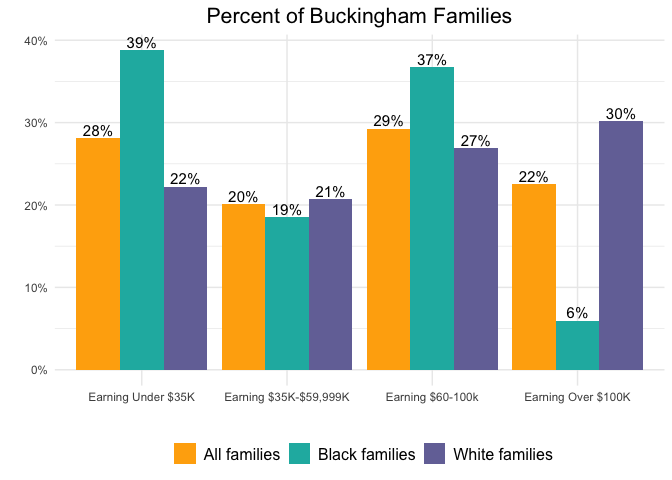
\includegraphics{orange-dot-test_files/figure-latex/unnamed-chunk-16-1} \end{center}

The maps below show the spatial relationship between income and
neighborhood. The color of each census tract in the county is based on
the median family income (the first map) or the percent of families
within the tract who make less than \$35,000 a year (the second map). In
Buckingham County, the median family income is low, relative to the
other counties, across all tracts.

To see which neighborhoods in Buckingham County have the highest and
lowest median family incomes, click on each tract to see its median
income and neighborhood names.

\hypertarget{median-family-income-in-buckingham-county}{%
\subparagraph{Median Family Income in Buckingham
County}\label{median-family-income-in-buckingham-county}}

The New Canton tract has the lowest median family incomes at \$53,000.
However, relative to the other localities, the difference between the
lowest median family income and the highest median family income in
Buckingham is small---the Mount Rush tract has the highest median family
income (\$76,196).

The following map shows the concentration of low-paid families. In
Buckingham County, the tract with the lowest median family income also
has the highest percentage of families making under \$35,000.

\hypertarget{percent-of-families-making-under-35000-in-buckingham-county}{%
\subparagraph{Percent of Families Making under \$35,000 in Buckingham
County}\label{percent-of-families-making-under-35000-in-buckingham-county}}

\protect\hyperlink{localities}{Return to Localities ↩︎}

\hypertarget{charlottesville-city}{%
\paragraph{Charlottesville City}\label{charlottesville-city}}

\hypertarget{charlottesville-city-1}{%
\subparagraph{Charlottesville City}\label{charlottesville-city-1}}

There are 8,950 families living in the city of Charlottesville. Of
these, 1,710 (19.1\%) do not earn enough to provide for their basic
needs and the costs associated with working.

Charlottesville City at a glance:

\begin{itemize}
\item
  Charlottesville and Albemarle County are the most expensive localities
  in the region given the costs of housing and childcare.
\item
  Charlottesville has the largest racial disparity among struggling
  families; the percent of Black families making under \$35,000 (48\%)
  is 36\% higher than the percent of white families making under
  \$35,000 (12\%).
\item
  Families making less than \$35,000 a year tend to be more highly
  concentrated near the University of Virginia, in the 10th \& Page and
  Venable neighborhoods and the JPA and Fontaine neighborhoods.
\end{itemize}

\hypertarget{expenses-single-householder-2-children-1-toddler-2}{%
\subparagraph{Expenses: Single Householder + 2 Children (1
Toddler)}\label{expenses-single-householder-2-children-1-toddler-2}}

\global\setlength{\Oldarrayrulewidth}{\arrayrulewidth}

\global\setlength{\Oldtabcolsep}{\tabcolsep}

\setlength{\tabcolsep}{0pt}

\renewcommand*{\arraystretch}{1.5}



\providecommand{\ascline}[3]{\noalign{\global\arrayrulewidth #1}\arrayrulecolor[HTML]{#2}\cline{#3}}

\begin{longtable}[c]{|p{5.00in}|p{5.00in}|p{5.00in}|p{5.00in}}



\hhline{>{\arrayrulecolor[HTML]{666666}\global\arrayrulewidth=2pt}->{\arrayrulecolor[HTML]{666666}\global\arrayrulewidth=2pt}->{\arrayrulecolor[HTML]{666666}\global\arrayrulewidth=2pt}->{\arrayrulecolor[HTML]{666666}\global\arrayrulewidth=2pt}-}

\multicolumn{1}{>{\cellcolor[HTML]{FFFFFF}\centering}p{\dimexpr 5in+0\tabcolsep}}{\textcolor[HTML]{000000}{\fontsize{11}{11}\selectfont{Expense}}} & \multicolumn{1}{>{\cellcolor[HTML]{FFFFFF}\centering}p{\dimexpr 5in+0\tabcolsep}}{\textcolor[HTML]{000000}{\fontsize{11}{11}\selectfont{Annual}}} & \multicolumn{1}{>{\cellcolor[HTML]{FFFFFF}\centering}p{\dimexpr 5in+0\tabcolsep}}{\textcolor[HTML]{000000}{\fontsize{11}{11}\selectfont{Monthly}}} & \multicolumn{1}{>{\cellcolor[HTML]{FFFFFF}\centering}p{\dimexpr 5in+0\tabcolsep}}{\textcolor[HTML]{000000}{\fontsize{11}{11}\selectfont{Weekly}}} \\

\noalign{\global\arrayrulewidth 0pt}\arrayrulecolor[HTML]{000000}

\hhline{>{\arrayrulecolor[HTML]{666666}\global\arrayrulewidth=2pt}->{\arrayrulecolor[HTML]{666666}\global\arrayrulewidth=2pt}->{\arrayrulecolor[HTML]{666666}\global\arrayrulewidth=2pt}->{\arrayrulecolor[HTML]{666666}\global\arrayrulewidth=2pt}-}\endhead



\multicolumn{1}{>{\cellcolor[HTML]{FFFFFF}\centering}p{\dimexpr 5in+0\tabcolsep}}{\textcolor[HTML]{000000}{\fontsize{11}{11}\selectfont{Food}}} & \multicolumn{1}{>{\cellcolor[HTML]{FFFFFF}\centering}p{\dimexpr 5in+0\tabcolsep}}{\textcolor[HTML]{000000}{\fontsize{11}{11}\selectfont{6,630.0}}} & \multicolumn{1}{>{\cellcolor[HTML]{FFFFFF}\centering}p{\dimexpr 5in+0\tabcolsep}}{\textcolor[HTML]{000000}{\fontsize{11}{11}\selectfont{552.50}}} & \multicolumn{1}{>{\cellcolor[HTML]{FFFFFF}\centering}p{\dimexpr 5in+0\tabcolsep}}{\textcolor[HTML]{000000}{\fontsize{11}{11}\selectfont{127.50}}} \\

\noalign{\global\arrayrulewidth 0pt}\arrayrulecolor[HTML]{000000}

\hhline{>{\arrayrulecolor[HTML]{BEBEBE}\global\arrayrulewidth=1pt}->{\arrayrulecolor[HTML]{BEBEBE}\global\arrayrulewidth=1pt}->{\arrayrulecolor[HTML]{BEBEBE}\global\arrayrulewidth=1pt}->{\arrayrulecolor[HTML]{BEBEBE}\global\arrayrulewidth=1pt}-}



\multicolumn{1}{>{\cellcolor[HTML]{FFFFFF}\centering}p{\dimexpr 5in+0\tabcolsep}}{\textcolor[HTML]{000000}{\fontsize{11}{11}\selectfont{Clothing}}} & \multicolumn{1}{>{\cellcolor[HTML]{FFFFFF}\centering}p{\dimexpr 5in+0\tabcolsep}}{\textcolor[HTML]{000000}{\fontsize{11}{11}\selectfont{2,334.0}}} & \multicolumn{1}{>{\cellcolor[HTML]{FFFFFF}\centering}p{\dimexpr 5in+0\tabcolsep}}{\textcolor[HTML]{000000}{\fontsize{11}{11}\selectfont{194.50}}} & \multicolumn{1}{>{\cellcolor[HTML]{FFFFFF}\centering}p{\dimexpr 5in+0\tabcolsep}}{\textcolor[HTML]{000000}{\fontsize{11}{11}\selectfont{44.88}}} \\

\noalign{\global\arrayrulewidth 0pt}\arrayrulecolor[HTML]{000000}

\hhline{>{\arrayrulecolor[HTML]{BEBEBE}\global\arrayrulewidth=1pt}->{\arrayrulecolor[HTML]{BEBEBE}\global\arrayrulewidth=1pt}->{\arrayrulecolor[HTML]{BEBEBE}\global\arrayrulewidth=1pt}->{\arrayrulecolor[HTML]{BEBEBE}\global\arrayrulewidth=1pt}-}



\multicolumn{1}{>{\cellcolor[HTML]{FFFFFF}\centering}p{\dimexpr 5in+0\tabcolsep}}{\textcolor[HTML]{000000}{\fontsize{11}{11}\selectfont{Shelter}}} & \multicolumn{1}{>{\cellcolor[HTML]{FFFFFF}\centering}p{\dimexpr 5in+0\tabcolsep}}{\textcolor[HTML]{000000}{\fontsize{11}{11}\selectfont{15,168.0}}} & \multicolumn{1}{>{\cellcolor[HTML]{FFFFFF}\centering}p{\dimexpr 5in+0\tabcolsep}}{\textcolor[HTML]{000000}{\fontsize{11}{11}\selectfont{1,264.00}}} & \multicolumn{1}{>{\cellcolor[HTML]{FFFFFF}\centering}p{\dimexpr 5in+0\tabcolsep}}{\textcolor[HTML]{000000}{\fontsize{11}{11}\selectfont{291.69}}} \\

\noalign{\global\arrayrulewidth 0pt}\arrayrulecolor[HTML]{000000}

\hhline{>{\arrayrulecolor[HTML]{BEBEBE}\global\arrayrulewidth=1pt}->{\arrayrulecolor[HTML]{BEBEBE}\global\arrayrulewidth=1pt}->{\arrayrulecolor[HTML]{BEBEBE}\global\arrayrulewidth=1pt}->{\arrayrulecolor[HTML]{BEBEBE}\global\arrayrulewidth=1pt}-}



\multicolumn{1}{>{\cellcolor[HTML]{FFFFFF}\centering}p{\dimexpr 5in+0\tabcolsep}}{\textcolor[HTML]{000000}{\fontsize{11}{11}\selectfont{Utilities}}} & \multicolumn{1}{>{\cellcolor[HTML]{FFFFFF}\centering}p{\dimexpr 5in+0\tabcolsep}}{\textcolor[HTML]{000000}{\fontsize{11}{11}\selectfont{3,325.0}}} & \multicolumn{1}{>{\cellcolor[HTML]{FFFFFF}\centering}p{\dimexpr 5in+0\tabcolsep}}{\textcolor[HTML]{000000}{\fontsize{11}{11}\selectfont{277.08}}} & \multicolumn{1}{>{\cellcolor[HTML]{FFFFFF}\centering}p{\dimexpr 5in+0\tabcolsep}}{\textcolor[HTML]{000000}{\fontsize{11}{11}\selectfont{63.94}}} \\

\noalign{\global\arrayrulewidth 0pt}\arrayrulecolor[HTML]{000000}

\hhline{>{\arrayrulecolor[HTML]{BEBEBE}\global\arrayrulewidth=1pt}->{\arrayrulecolor[HTML]{BEBEBE}\global\arrayrulewidth=1pt}->{\arrayrulecolor[HTML]{BEBEBE}\global\arrayrulewidth=1pt}->{\arrayrulecolor[HTML]{BEBEBE}\global\arrayrulewidth=1pt}-}



\multicolumn{1}{>{\cellcolor[HTML]{FFFFFF}\centering}p{\dimexpr 5in+0\tabcolsep}}{\textcolor[HTML]{000000}{\fontsize{11}{11}\selectfont{Necessary\ Costs}}} & \multicolumn{1}{>{\cellcolor[HTML]{FFFFFF}\centering}p{\dimexpr 5in+0\tabcolsep}}{\textcolor[HTML]{000000}{\fontsize{11}{11}\selectfont{5,491.4}}} & \multicolumn{1}{>{\cellcolor[HTML]{FFFFFF}\centering}p{\dimexpr 5in+0\tabcolsep}}{\textcolor[HTML]{000000}{\fontsize{11}{11}\selectfont{457.62}}} & \multicolumn{1}{>{\cellcolor[HTML]{FFFFFF}\centering}p{\dimexpr 5in+0\tabcolsep}}{\textcolor[HTML]{000000}{\fontsize{11}{11}\selectfont{105.60}}} \\

\noalign{\global\arrayrulewidth 0pt}\arrayrulecolor[HTML]{000000}

\hhline{>{\arrayrulecolor[HTML]{BEBEBE}\global\arrayrulewidth=1pt}->{\arrayrulecolor[HTML]{BEBEBE}\global\arrayrulewidth=1pt}->{\arrayrulecolor[HTML]{BEBEBE}\global\arrayrulewidth=1pt}->{\arrayrulecolor[HTML]{BEBEBE}\global\arrayrulewidth=1pt}-}



\multicolumn{1}{>{\cellcolor[HTML]{FFAD0A}\centering}p{\dimexpr 5in+0\tabcolsep}}{\textcolor[HTML]{000000}{\fontsize{11}{11}\selectfont{Survival\ Expenses}}} & \multicolumn{1}{>{\cellcolor[HTML]{FFAD0A}\centering}p{\dimexpr 5in+0\tabcolsep}}{\textcolor[HTML]{000000}{\fontsize{11}{11}\selectfont{32,948.4}}} & \multicolumn{1}{>{\cellcolor[HTML]{FFAD0A}\centering}p{\dimexpr 5in+0\tabcolsep}}{\textcolor[HTML]{000000}{\fontsize{11}{11}\selectfont{2,745.70}}} & \multicolumn{1}{>{\cellcolor[HTML]{FFAD0A}\centering}p{\dimexpr 5in+0\tabcolsep}}{\textcolor[HTML]{000000}{\fontsize{11}{11}\selectfont{633.62}}} \\

\noalign{\global\arrayrulewidth 0pt}\arrayrulecolor[HTML]{000000}

\hhline{>{\arrayrulecolor[HTML]{BEBEBE}\global\arrayrulewidth=1pt}->{\arrayrulecolor[HTML]{BEBEBE}\global\arrayrulewidth=1pt}->{\arrayrulecolor[HTML]{BEBEBE}\global\arrayrulewidth=1pt}->{\arrayrulecolor[HTML]{BEBEBE}\global\arrayrulewidth=1pt}-}



\multicolumn{1}{>{\cellcolor[HTML]{FFFFFF}\centering}p{\dimexpr 5in+0\tabcolsep}}{\textcolor[HTML]{000000}{\fontsize{11}{11}\selectfont{Childcare}}} & \multicolumn{1}{>{\cellcolor[HTML]{FFFFFF}\centering}p{\dimexpr 5in+0\tabcolsep}}{\textcolor[HTML]{000000}{\fontsize{11}{11}\selectfont{21,580.0}}} & \multicolumn{1}{>{\cellcolor[HTML]{FFFFFF}\centering}p{\dimexpr 5in+0\tabcolsep}}{\textcolor[HTML]{000000}{\fontsize{11}{11}\selectfont{1,798.00}}} & \multicolumn{1}{>{\cellcolor[HTML]{FFFFFF}\centering}p{\dimexpr 5in+0\tabcolsep}}{\textcolor[HTML]{000000}{\fontsize{11}{11}\selectfont{415.00}}} \\

\noalign{\global\arrayrulewidth 0pt}\arrayrulecolor[HTML]{000000}

\hhline{>{\arrayrulecolor[HTML]{BEBEBE}\global\arrayrulewidth=1pt}->{\arrayrulecolor[HTML]{BEBEBE}\global\arrayrulewidth=1pt}->{\arrayrulecolor[HTML]{BEBEBE}\global\arrayrulewidth=1pt}->{\arrayrulecolor[HTML]{BEBEBE}\global\arrayrulewidth=1pt}-}



\multicolumn{1}{>{\cellcolor[HTML]{FFFFFF}\centering}p{\dimexpr 5in+0\tabcolsep}}{\textcolor[HTML]{000000}{\fontsize{11}{11}\selectfont{Transportation}}} & \multicolumn{1}{>{\cellcolor[HTML]{FFFFFF}\centering}p{\dimexpr 5in+0\tabcolsep}}{\textcolor[HTML]{000000}{\fontsize{11}{11}\selectfont{3,996.0}}} & \multicolumn{1}{>{\cellcolor[HTML]{FFFFFF}\centering}p{\dimexpr 5in+0\tabcolsep}}{\textcolor[HTML]{000000}{\fontsize{11}{11}\selectfont{333.00}}} & \multicolumn{1}{>{\cellcolor[HTML]{FFFFFF}\centering}p{\dimexpr 5in+0\tabcolsep}}{\textcolor[HTML]{000000}{\fontsize{11}{11}\selectfont{76.85}}} \\

\noalign{\global\arrayrulewidth 0pt}\arrayrulecolor[HTML]{000000}

\hhline{>{\arrayrulecolor[HTML]{BEBEBE}\global\arrayrulewidth=1pt}->{\arrayrulecolor[HTML]{BEBEBE}\global\arrayrulewidth=1pt}->{\arrayrulecolor[HTML]{BEBEBE}\global\arrayrulewidth=1pt}->{\arrayrulecolor[HTML]{BEBEBE}\global\arrayrulewidth=1pt}-}



\multicolumn{1}{>{\cellcolor[HTML]{EE6100}\centering}p{\dimexpr 5in+0\tabcolsep}}{\textcolor[HTML]{FFFFFF}{\fontsize{11}{11}\selectfont{Total\ Expenses}}} & \multicolumn{1}{>{\cellcolor[HTML]{EE6100}\centering}p{\dimexpr 5in+0\tabcolsep}}{\textcolor[HTML]{FFFFFF}{\fontsize{11}{11}\selectfont{58,524.4}}} & \multicolumn{1}{>{\cellcolor[HTML]{EE6100}\centering}p{\dimexpr 5in+0\tabcolsep}}{\textcolor[HTML]{FFFFFF}{\fontsize{11}{11}\selectfont{4,116.20}}} & \multicolumn{1}{>{\cellcolor[HTML]{EE6100}\centering}p{\dimexpr 5in+0\tabcolsep}}{\textcolor[HTML]{FFFFFF}{\fontsize{11}{11}\selectfont{949.89}}} \\

\noalign{\global\arrayrulewidth 0pt}\arrayrulecolor[HTML]{000000}

\hhline{>{\arrayrulecolor[HTML]{666666}\global\arrayrulewidth=2pt}->{\arrayrulecolor[HTML]{666666}\global\arrayrulewidth=2pt}->{\arrayrulecolor[HTML]{666666}\global\arrayrulewidth=2pt}->{\arrayrulecolor[HTML]{666666}\global\arrayrulewidth=2pt}-}



\end{longtable}



\arrayrulecolor[HTML]{000000}

\global\setlength{\arrayrulewidth}{\Oldarrayrulewidth}

\global\setlength{\tabcolsep}{\Oldtabcolsep}

\renewcommand*{\arraystretch}{1}

\hypertarget{breakdown-of-families-making-under-35000-in-charlottesville-city}{%
\subparagraph{Breakdown of Families Making under \$35,000 in
Charlottesville
City}\label{breakdown-of-families-making-under-35000-in-charlottesville-city}}

\global\setlength{\Oldarrayrulewidth}{\arrayrulewidth}

\global\setlength{\Oldtabcolsep}{\tabcolsep}

\setlength{\tabcolsep}{0pt}

\renewcommand*{\arraystretch}{1.5}



\providecommand{\ascline}[3]{\noalign{\global\arrayrulewidth #1}\arrayrulecolor[HTML]{#2}\cline{#3}}

\begin{longtable}[c]{|p{5.00in}|p{5.00in}|p{5.00in}|p{5.00in}}



\hhline{>{\arrayrulecolor[HTML]{666666}\global\arrayrulewidth=2pt}->{\arrayrulecolor[HTML]{666666}\global\arrayrulewidth=2pt}->{\arrayrulecolor[HTML]{666666}\global\arrayrulewidth=2pt}->{\arrayrulecolor[HTML]{666666}\global\arrayrulewidth=2pt}-}

\multicolumn{1}{>{\cellcolor[HTML]{FFFFFF}\centering}p{\dimexpr 5in+0\tabcolsep}}{\textcolor[HTML]{000000}{\fontsize{11}{11}\selectfont{Income}}} & \multicolumn{1}{>{\cellcolor[HTML]{FFFFFF}\centering}p{\dimexpr 5in+0\tabcolsep}}{\textcolor[HTML]{000000}{\fontsize{11}{11}\selectfont{Number}}} & \multicolumn{1}{>{\cellcolor[HTML]{FFFFFF}\centering}p{\dimexpr 5in+0\tabcolsep}}{\textcolor[HTML]{000000}{\fontsize{11}{11}\selectfont{Percent}}} & \multicolumn{1}{>{\cellcolor[HTML]{FFFFFF}\centering}p{\dimexpr 5in+0\tabcolsep}}{\textcolor[HTML]{000000}{\fontsize{11}{11}\selectfont{Cumulative}}} \\

\noalign{\global\arrayrulewidth 0pt}\arrayrulecolor[HTML]{000000}

\hhline{>{\arrayrulecolor[HTML]{666666}\global\arrayrulewidth=2pt}->{\arrayrulecolor[HTML]{666666}\global\arrayrulewidth=2pt}->{\arrayrulecolor[HTML]{666666}\global\arrayrulewidth=2pt}->{\arrayrulecolor[HTML]{666666}\global\arrayrulewidth=2pt}-}\endhead



\multicolumn{1}{>{\cellcolor[HTML]{FFFFFF}\centering}p{\dimexpr 5in+0\tabcolsep}}{\textcolor[HTML]{000000}{\fontsize{11}{11}\selectfont{\$0\ -\ \$9,999}}} & \multicolumn{1}{>{\cellcolor[HTML]{FFFFFF}\centering}p{\dimexpr 5in+0\tabcolsep}}{\textcolor[HTML]{000000}{\fontsize{11}{11}\selectfont{480}}} & \multicolumn{1}{>{\cellcolor[HTML]{FFFFFF}\centering}p{\dimexpr 5in+0\tabcolsep}}{\textcolor[HTML]{000000}{\fontsize{11}{11}\selectfont{28\%}}} & \multicolumn{1}{>{\cellcolor[HTML]{FFAD0A}\centering}p{\dimexpr 5in+0\tabcolsep}}{} \\

\noalign{\global\arrayrulewidth 0pt}\arrayrulecolor[HTML]{000000}

\hhline{>{\arrayrulecolor[HTML]{BEBEBE}\global\arrayrulewidth=1pt}->{\arrayrulecolor[HTML]{BEBEBE}\global\arrayrulewidth=1pt}->{\arrayrulecolor[HTML]{BEBEBE}\global\arrayrulewidth=1pt}->{\arrayrulecolor[HTML]{FFAD0A}\global\arrayrulewidth=1pt}-}



\multicolumn{1}{>{\cellcolor[HTML]{FFFFFF}\centering}p{\dimexpr 5in+0\tabcolsep}}{\textcolor[HTML]{000000}{\fontsize{11}{11}\selectfont{\$10,000\ -\ \$14,999}}} & \multicolumn{1}{>{\cellcolor[HTML]{FFFFFF}\centering}p{\dimexpr 5in+0\tabcolsep}}{\textcolor[HTML]{000000}{\fontsize{11}{11}\selectfont{238}}} & \multicolumn{1}{>{\cellcolor[HTML]{FFFFFF}\centering}p{\dimexpr 5in+0\tabcolsep}}{\textcolor[HTML]{000000}{\fontsize{11}{11}\selectfont{14\%}}} & \multicolumn{1}{>{\cellcolor[HTML]{FFAD0A}\centering}p{\dimexpr 5in+0\tabcolsep}}{\multirow[c]{-2}{*}{\parbox{5in}{\textcolor[HTML]{000000}{\fontsize{11}{11}\selectfont{42\%}}}}} \\

\noalign{\global\arrayrulewidth 0pt}\arrayrulecolor[HTML]{000000}

\hhline{>{\arrayrulecolor[HTML]{BEBEBE}\global\arrayrulewidth=1pt}->{\arrayrulecolor[HTML]{BEBEBE}\global\arrayrulewidth=1pt}->{\arrayrulecolor[HTML]{BEBEBE}\global\arrayrulewidth=1pt}->{\arrayrulecolor[HTML]{BEBEBE}\global\arrayrulewidth=1pt}-}



\multicolumn{1}{>{\cellcolor[HTML]{FFFFFF}\centering}p{\dimexpr 5in+0\tabcolsep}}{\textcolor[HTML]{000000}{\fontsize{11}{11}\selectfont{\$15,000\ -\ \$24,999}}} & \multicolumn{1}{>{\cellcolor[HTML]{FFFFFF}\centering}p{\dimexpr 5in+0\tabcolsep}}{\textcolor[HTML]{000000}{\fontsize{11}{11}\selectfont{417}}} & \multicolumn{1}{>{\cellcolor[HTML]{FFFFFF}\centering}p{\dimexpr 5in+0\tabcolsep}}{\textcolor[HTML]{000000}{\fontsize{11}{11}\selectfont{24\%}}} & \multicolumn{1}{>{\cellcolor[HTML]{EE6100}\centering}p{\dimexpr 5in+0\tabcolsep}}{} \\

\noalign{\global\arrayrulewidth 0pt}\arrayrulecolor[HTML]{000000}

\hhline{>{\arrayrulecolor[HTML]{BEBEBE}\global\arrayrulewidth=1pt}->{\arrayrulecolor[HTML]{BEBEBE}\global\arrayrulewidth=1pt}->{\arrayrulecolor[HTML]{BEBEBE}\global\arrayrulewidth=1pt}->{\arrayrulecolor[HTML]{EE6100}\global\arrayrulewidth=1pt}-}



\multicolumn{1}{>{\cellcolor[HTML]{FFFFFF}\centering}p{\dimexpr 5in+0\tabcolsep}}{\textcolor[HTML]{000000}{\fontsize{11}{11}\selectfont{\$25,000\ -\ \$34,999}}} & \multicolumn{1}{>{\cellcolor[HTML]{FFFFFF}\centering}p{\dimexpr 5in+0\tabcolsep}}{\textcolor[HTML]{000000}{\fontsize{11}{11}\selectfont{575}}} & \multicolumn{1}{>{\cellcolor[HTML]{FFFFFF}\centering}p{\dimexpr 5in+0\tabcolsep}}{\textcolor[HTML]{000000}{\fontsize{11}{11}\selectfont{34\%}}} & \multicolumn{1}{>{\cellcolor[HTML]{EE6100}\centering}p{\dimexpr 5in+0\tabcolsep}}{\multirow[c]{-2}{*}{\parbox{5in}{\textcolor[HTML]{FFFFFF}{\fontsize{11}{11}\selectfont{58\%}}}}} \\

\noalign{\global\arrayrulewidth 0pt}\arrayrulecolor[HTML]{000000}

\hhline{>{\arrayrulecolor[HTML]{BEBEBE}\global\arrayrulewidth=1pt}->{\arrayrulecolor[HTML]{BEBEBE}\global\arrayrulewidth=1pt}->{\arrayrulecolor[HTML]{BEBEBE}\global\arrayrulewidth=1pt}->{\arrayrulecolor[HTML]{BEBEBE}\global\arrayrulewidth=1pt}-}



\multicolumn{1}{>{\cellcolor[HTML]{FFFFFF}\centering}p{\dimexpr 5in+0\tabcolsep}}{\textcolor[HTML]{000000}{\fontsize{11}{11}\selectfont{Total}}} & \multicolumn{1}{>{\cellcolor[HTML]{FFFFFF}\centering}p{\dimexpr 5in+0\tabcolsep}}{\textcolor[HTML]{000000}{\fontsize{11}{11}\selectfont{1,710}}} & \multicolumn{2}{>{\cellcolor[HTML]{FFFFFF}\centering}p{\dimexpr 10in+2\tabcolsep}}{\textcolor[HTML]{000000}{\fontsize{11}{11}\selectfont{100\%}}} \\

\noalign{\global\arrayrulewidth 0pt}\arrayrulecolor[HTML]{000000}

\hhline{>{\arrayrulecolor[HTML]{666666}\global\arrayrulewidth=2pt}->{\arrayrulecolor[HTML]{666666}\global\arrayrulewidth=2pt}->{\arrayrulecolor[HTML]{666666}\global\arrayrulewidth=2pt}->{\arrayrulecolor[HTML]{666666}\global\arrayrulewidth=2pt}-}



\end{longtable}



\arrayrulecolor[HTML]{000000}

\global\setlength{\arrayrulewidth}{\Oldarrayrulewidth}

\global\setlength{\tabcolsep}{\Oldtabcolsep}

\renewcommand*{\arraystretch}{1}

As this table shows, 58\% of the families who cannot meet their basic
needs earn between \$15,000-\$35,000 annually. This strongly suggests
they are working, but not earning the wages or not getting the hours
they need to support their families. In Charlottesville, however, the
percent of families making under \$35,000 a year are more evenly
distributed across the \$0-\$14,999 and \$15,000-\$34,999 ranges. This
distribution means that more families, relative to the other localities,
are in the lowest income range.

The figure below shows the distribution of families in various pay
ranges, disaggregated by race. In a world with racial equity in income,
the bars for all families would be equal in height. In Charlottesville,
Black families are highly over-represented at the low end of the pay
ranges (under \$35,000 a year) and under-represented at the high end of
the pay ranges (over \$100,000 a year). In other words, relative to
white families, Black families are more likely to be paid insufficient
wages and less likely to be high-earning.

\hypertarget{income-distribution-of-black-and-white-families-in-charlottesville-city}{%
\subparagraph{Income Distribution of Black and White Families in
Charlottesville
City}\label{income-distribution-of-black-and-white-families-in-charlottesville-city}}

\begin{center}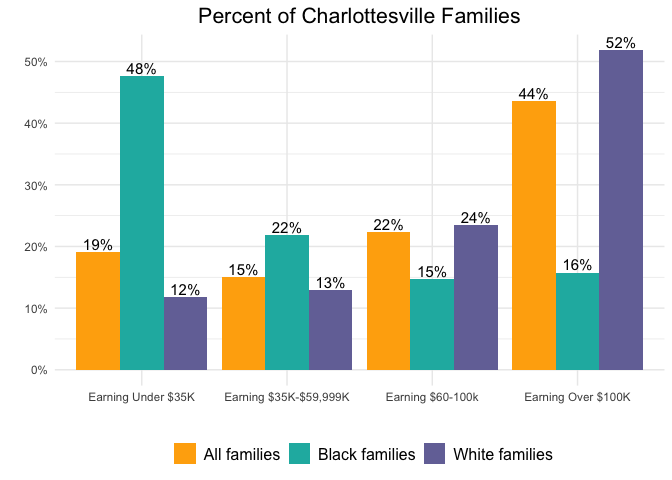
\includegraphics{orange-dot-test_files/figure-latex/unnamed-chunk-22-1} \end{center}

The maps below show the spatial relationship between income and
neighborhood. The color of each census tract in the county is based on
the median family income or the percent of families within the tract who
make less than \$35,000. The maps show how residents are often
concentrated into neighborhoods with either high-earning or low-earning
families, with implications for the resources and opportunities
available to the families living within each tract.

To see which neighborhoods in the city of Charlottesville have the
highest and lowest median family incomes, click on each tract to see its
median income and neighborhood names.

\hypertarget{median-family-income-in-charlottesville-city}{%
\subparagraph{Median Family Income in Charlottesville
City}\label{median-family-income-in-charlottesville-city}}

The 10th \& Page-Venable tract has the lowest median family incomes at
\$31,857. By contrast, the Barracks-Rugby tract has the highest median
family income at \$171,250, making the disparity between the lowest and
highest median family incomes well-over \$100k.

The following map shows the concentration of low-paid families. For
Charlottesville, it shows a similar pattern as the previous map---the
highest percentage of low-paid families are concentrated in the 10th \&
Page-Venable and JPA-Fontaine tracts. The Barracks-Rugby tract, in
addition to having the highest median family income, also has the lowest
percent of families making less than \$35,000.

\hypertarget{percent-of-families-making-under-35000-in-charlottesville-city}{%
\subparagraph{Percent of Families Making under \$35,000 in
Charlottesville
City}\label{percent-of-families-making-under-35000-in-charlottesville-city}}

\protect\hyperlink{localities}{Return to Localities ↩︎}

\hypertarget{fluvanna-county}{%
\paragraph{Fluvanna County}\label{fluvanna-county}}

\hypertarget{fluvanna-county-1}{%
\subparagraph{Fluvanna County}\label{fluvanna-county-1}}

There are 7,131 families living in Fluvanna County. Of these, 559
(7.8\%) do not earn enough to provide for their basic needs and the
costs associated with working.

Fluvanna County at a glance:

\begin{itemize}
\item
  Fluvanna ranks as the third most expensive locality for families in
  the region given the costs of housing and childcare.
\item
  Fluvanna has the lowest percent of struggling families across the
  region, and the smallest racial disparity across struggling families.
  The percent of Black families making under \$35,000 (11\%) is 4\%
  higher than the percent of white families making under \$35,000 (7\%).
\item
  Fluvanna, relative to the other localities, has the largest percent of
  families making in the \$60,000-\$100,000 a year range, and the second
  largest percent of families making over \$100,000.
\item
  Relative to the other counties, the spatial difference between the
  highest median family income in a tract and the lowest is smaller in
  Fluvanna. In other words, the median family income is more consistent
  across the areas in Fluvanna than it is in other counties.
\end{itemize}

\hypertarget{expenses-single-householder-2-children-1-toddler-3}{%
\subparagraph{Expenses: Single Householder + 2 Children (1
Toddler)}\label{expenses-single-householder-2-children-1-toddler-3}}

\global\setlength{\Oldarrayrulewidth}{\arrayrulewidth}

\global\setlength{\Oldtabcolsep}{\tabcolsep}

\setlength{\tabcolsep}{0pt}

\renewcommand*{\arraystretch}{1.5}



\providecommand{\ascline}[3]{\noalign{\global\arrayrulewidth #1}\arrayrulecolor[HTML]{#2}\cline{#3}}

\begin{longtable}[c]{|p{5.00in}|p{5.00in}|p{5.00in}|p{5.00in}}



\hhline{>{\arrayrulecolor[HTML]{666666}\global\arrayrulewidth=2pt}->{\arrayrulecolor[HTML]{666666}\global\arrayrulewidth=2pt}->{\arrayrulecolor[HTML]{666666}\global\arrayrulewidth=2pt}->{\arrayrulecolor[HTML]{666666}\global\arrayrulewidth=2pt}-}

\multicolumn{1}{>{\cellcolor[HTML]{FFFFFF}\centering}p{\dimexpr 5in+0\tabcolsep}}{\textcolor[HTML]{000000}{\fontsize{11}{11}\selectfont{Expense}}} & \multicolumn{1}{>{\cellcolor[HTML]{FFFFFF}\centering}p{\dimexpr 5in+0\tabcolsep}}{\textcolor[HTML]{000000}{\fontsize{11}{11}\selectfont{Annual}}} & \multicolumn{1}{>{\cellcolor[HTML]{FFFFFF}\centering}p{\dimexpr 5in+0\tabcolsep}}{\textcolor[HTML]{000000}{\fontsize{11}{11}\selectfont{Monthly}}} & \multicolumn{1}{>{\cellcolor[HTML]{FFFFFF}\centering}p{\dimexpr 5in+0\tabcolsep}}{\textcolor[HTML]{000000}{\fontsize{11}{11}\selectfont{Weekly}}} \\

\noalign{\global\arrayrulewidth 0pt}\arrayrulecolor[HTML]{000000}

\hhline{>{\arrayrulecolor[HTML]{666666}\global\arrayrulewidth=2pt}->{\arrayrulecolor[HTML]{666666}\global\arrayrulewidth=2pt}->{\arrayrulecolor[HTML]{666666}\global\arrayrulewidth=2pt}->{\arrayrulecolor[HTML]{666666}\global\arrayrulewidth=2pt}-}\endhead



\multicolumn{1}{>{\cellcolor[HTML]{FFFFFF}\centering}p{\dimexpr 5in+0\tabcolsep}}{\textcolor[HTML]{000000}{\fontsize{11}{11}\selectfont{Food}}} & \multicolumn{1}{>{\cellcolor[HTML]{FFFFFF}\centering}p{\dimexpr 5in+0\tabcolsep}}{\textcolor[HTML]{000000}{\fontsize{11}{11}\selectfont{6,630.0}}} & \multicolumn{1}{>{\cellcolor[HTML]{FFFFFF}\centering}p{\dimexpr 5in+0\tabcolsep}}{\textcolor[HTML]{000000}{\fontsize{11}{11}\selectfont{552.50}}} & \multicolumn{1}{>{\cellcolor[HTML]{FFFFFF}\centering}p{\dimexpr 5in+0\tabcolsep}}{\textcolor[HTML]{000000}{\fontsize{11}{11}\selectfont{127.50}}} \\

\noalign{\global\arrayrulewidth 0pt}\arrayrulecolor[HTML]{000000}

\hhline{>{\arrayrulecolor[HTML]{BEBEBE}\global\arrayrulewidth=1pt}->{\arrayrulecolor[HTML]{BEBEBE}\global\arrayrulewidth=1pt}->{\arrayrulecolor[HTML]{BEBEBE}\global\arrayrulewidth=1pt}->{\arrayrulecolor[HTML]{BEBEBE}\global\arrayrulewidth=1pt}-}



\multicolumn{1}{>{\cellcolor[HTML]{FFFFFF}\centering}p{\dimexpr 5in+0\tabcolsep}}{\textcolor[HTML]{000000}{\fontsize{11}{11}\selectfont{Clothing}}} & \multicolumn{1}{>{\cellcolor[HTML]{FFFFFF}\centering}p{\dimexpr 5in+0\tabcolsep}}{\textcolor[HTML]{000000}{\fontsize{11}{11}\selectfont{2,334.0}}} & \multicolumn{1}{>{\cellcolor[HTML]{FFFFFF}\centering}p{\dimexpr 5in+0\tabcolsep}}{\textcolor[HTML]{000000}{\fontsize{11}{11}\selectfont{194.50}}} & \multicolumn{1}{>{\cellcolor[HTML]{FFFFFF}\centering}p{\dimexpr 5in+0\tabcolsep}}{\textcolor[HTML]{000000}{\fontsize{11}{11}\selectfont{44.88}}} \\

\noalign{\global\arrayrulewidth 0pt}\arrayrulecolor[HTML]{000000}

\hhline{>{\arrayrulecolor[HTML]{BEBEBE}\global\arrayrulewidth=1pt}->{\arrayrulecolor[HTML]{BEBEBE}\global\arrayrulewidth=1pt}->{\arrayrulecolor[HTML]{BEBEBE}\global\arrayrulewidth=1pt}->{\arrayrulecolor[HTML]{BEBEBE}\global\arrayrulewidth=1pt}-}



\multicolumn{1}{>{\cellcolor[HTML]{FFFFFF}\centering}p{\dimexpr 5in+0\tabcolsep}}{\textcolor[HTML]{000000}{\fontsize{11}{11}\selectfont{Shelter}}} & \multicolumn{1}{>{\cellcolor[HTML]{FFFFFF}\centering}p{\dimexpr 5in+0\tabcolsep}}{\textcolor[HTML]{000000}{\fontsize{11}{11}\selectfont{15,168.0}}} & \multicolumn{1}{>{\cellcolor[HTML]{FFFFFF}\centering}p{\dimexpr 5in+0\tabcolsep}}{\textcolor[HTML]{000000}{\fontsize{11}{11}\selectfont{1,264.00}}} & \multicolumn{1}{>{\cellcolor[HTML]{FFFFFF}\centering}p{\dimexpr 5in+0\tabcolsep}}{\textcolor[HTML]{000000}{\fontsize{11}{11}\selectfont{291.69}}} \\

\noalign{\global\arrayrulewidth 0pt}\arrayrulecolor[HTML]{000000}

\hhline{>{\arrayrulecolor[HTML]{BEBEBE}\global\arrayrulewidth=1pt}->{\arrayrulecolor[HTML]{BEBEBE}\global\arrayrulewidth=1pt}->{\arrayrulecolor[HTML]{BEBEBE}\global\arrayrulewidth=1pt}->{\arrayrulecolor[HTML]{BEBEBE}\global\arrayrulewidth=1pt}-}



\multicolumn{1}{>{\cellcolor[HTML]{FFFFFF}\centering}p{\dimexpr 5in+0\tabcolsep}}{\textcolor[HTML]{000000}{\fontsize{11}{11}\selectfont{Utilities}}} & \multicolumn{1}{>{\cellcolor[HTML]{FFFFFF}\centering}p{\dimexpr 5in+0\tabcolsep}}{\textcolor[HTML]{000000}{\fontsize{11}{11}\selectfont{3,325.0}}} & \multicolumn{1}{>{\cellcolor[HTML]{FFFFFF}\centering}p{\dimexpr 5in+0\tabcolsep}}{\textcolor[HTML]{000000}{\fontsize{11}{11}\selectfont{277.08}}} & \multicolumn{1}{>{\cellcolor[HTML]{FFFFFF}\centering}p{\dimexpr 5in+0\tabcolsep}}{\textcolor[HTML]{000000}{\fontsize{11}{11}\selectfont{63.94}}} \\

\noalign{\global\arrayrulewidth 0pt}\arrayrulecolor[HTML]{000000}

\hhline{>{\arrayrulecolor[HTML]{BEBEBE}\global\arrayrulewidth=1pt}->{\arrayrulecolor[HTML]{BEBEBE}\global\arrayrulewidth=1pt}->{\arrayrulecolor[HTML]{BEBEBE}\global\arrayrulewidth=1pt}->{\arrayrulecolor[HTML]{BEBEBE}\global\arrayrulewidth=1pt}-}



\multicolumn{1}{>{\cellcolor[HTML]{FFFFFF}\centering}p{\dimexpr 5in+0\tabcolsep}}{\textcolor[HTML]{000000}{\fontsize{11}{11}\selectfont{Necessary\ Costs}}} & \multicolumn{1}{>{\cellcolor[HTML]{FFFFFF}\centering}p{\dimexpr 5in+0\tabcolsep}}{\textcolor[HTML]{000000}{\fontsize{11}{11}\selectfont{5,491.4}}} & \multicolumn{1}{>{\cellcolor[HTML]{FFFFFF}\centering}p{\dimexpr 5in+0\tabcolsep}}{\textcolor[HTML]{000000}{\fontsize{11}{11}\selectfont{457.62}}} & \multicolumn{1}{>{\cellcolor[HTML]{FFFFFF}\centering}p{\dimexpr 5in+0\tabcolsep}}{\textcolor[HTML]{000000}{\fontsize{11}{11}\selectfont{105.60}}} \\

\noalign{\global\arrayrulewidth 0pt}\arrayrulecolor[HTML]{000000}

\hhline{>{\arrayrulecolor[HTML]{BEBEBE}\global\arrayrulewidth=1pt}->{\arrayrulecolor[HTML]{BEBEBE}\global\arrayrulewidth=1pt}->{\arrayrulecolor[HTML]{BEBEBE}\global\arrayrulewidth=1pt}->{\arrayrulecolor[HTML]{BEBEBE}\global\arrayrulewidth=1pt}-}



\multicolumn{1}{>{\cellcolor[HTML]{FFAD0A}\centering}p{\dimexpr 5in+0\tabcolsep}}{\textcolor[HTML]{000000}{\fontsize{11}{11}\selectfont{Survival\ Expenses}}} & \multicolumn{1}{>{\cellcolor[HTML]{FFAD0A}\centering}p{\dimexpr 5in+0\tabcolsep}}{\textcolor[HTML]{000000}{\fontsize{11}{11}\selectfont{32,948.4}}} & \multicolumn{1}{>{\cellcolor[HTML]{FFAD0A}\centering}p{\dimexpr 5in+0\tabcolsep}}{\textcolor[HTML]{000000}{\fontsize{11}{11}\selectfont{2,745.70}}} & \multicolumn{1}{>{\cellcolor[HTML]{FFAD0A}\centering}p{\dimexpr 5in+0\tabcolsep}}{\textcolor[HTML]{000000}{\fontsize{11}{11}\selectfont{633.62}}} \\

\noalign{\global\arrayrulewidth 0pt}\arrayrulecolor[HTML]{000000}

\hhline{>{\arrayrulecolor[HTML]{BEBEBE}\global\arrayrulewidth=1pt}->{\arrayrulecolor[HTML]{BEBEBE}\global\arrayrulewidth=1pt}->{\arrayrulecolor[HTML]{BEBEBE}\global\arrayrulewidth=1pt}->{\arrayrulecolor[HTML]{BEBEBE}\global\arrayrulewidth=1pt}-}



\multicolumn{1}{>{\cellcolor[HTML]{FFFFFF}\centering}p{\dimexpr 5in+0\tabcolsep}}{\textcolor[HTML]{000000}{\fontsize{11}{11}\selectfont{Childcare}}} & \multicolumn{1}{>{\cellcolor[HTML]{FFFFFF}\centering}p{\dimexpr 5in+0\tabcolsep}}{\textcolor[HTML]{000000}{\fontsize{11}{11}\selectfont{15,080.0}}} & \multicolumn{1}{>{\cellcolor[HTML]{FFFFFF}\centering}p{\dimexpr 5in+0\tabcolsep}}{\textcolor[HTML]{000000}{\fontsize{11}{11}\selectfont{1,257.00}}} & \multicolumn{1}{>{\cellcolor[HTML]{FFFFFF}\centering}p{\dimexpr 5in+0\tabcolsep}}{\textcolor[HTML]{000000}{\fontsize{11}{11}\selectfont{290.00}}} \\

\noalign{\global\arrayrulewidth 0pt}\arrayrulecolor[HTML]{000000}

\hhline{>{\arrayrulecolor[HTML]{BEBEBE}\global\arrayrulewidth=1pt}->{\arrayrulecolor[HTML]{BEBEBE}\global\arrayrulewidth=1pt}->{\arrayrulecolor[HTML]{BEBEBE}\global\arrayrulewidth=1pt}->{\arrayrulecolor[HTML]{BEBEBE}\global\arrayrulewidth=1pt}-}



\multicolumn{1}{>{\cellcolor[HTML]{FFFFFF}\centering}p{\dimexpr 5in+0\tabcolsep}}{\textcolor[HTML]{000000}{\fontsize{11}{11}\selectfont{Transportation}}} & \multicolumn{1}{>{\cellcolor[HTML]{FFFFFF}\centering}p{\dimexpr 5in+0\tabcolsep}}{\textcolor[HTML]{000000}{\fontsize{11}{11}\selectfont{3,996.0}}} & \multicolumn{1}{>{\cellcolor[HTML]{FFFFFF}\centering}p{\dimexpr 5in+0\tabcolsep}}{\textcolor[HTML]{000000}{\fontsize{11}{11}\selectfont{333.00}}} & \multicolumn{1}{>{\cellcolor[HTML]{FFFFFF}\centering}p{\dimexpr 5in+0\tabcolsep}}{\textcolor[HTML]{000000}{\fontsize{11}{11}\selectfont{76.85}}} \\

\noalign{\global\arrayrulewidth 0pt}\arrayrulecolor[HTML]{000000}

\hhline{>{\arrayrulecolor[HTML]{BEBEBE}\global\arrayrulewidth=1pt}->{\arrayrulecolor[HTML]{BEBEBE}\global\arrayrulewidth=1pt}->{\arrayrulecolor[HTML]{BEBEBE}\global\arrayrulewidth=1pt}->{\arrayrulecolor[HTML]{BEBEBE}\global\arrayrulewidth=1pt}-}



\multicolumn{1}{>{\cellcolor[HTML]{EE6100}\centering}p{\dimexpr 5in+0\tabcolsep}}{\textcolor[HTML]{FFFFFF}{\fontsize{11}{11}\selectfont{Total\ Expenses}}} & \multicolumn{1}{>{\cellcolor[HTML]{EE6100}\centering}p{\dimexpr 5in+0\tabcolsep}}{\textcolor[HTML]{FFFFFF}{\fontsize{11}{11}\selectfont{52,024.4}}} & \multicolumn{1}{>{\cellcolor[HTML]{EE6100}\centering}p{\dimexpr 5in+0\tabcolsep}}{\textcolor[HTML]{FFFFFF}{\fontsize{11}{11}\selectfont{4,116.20}}} & \multicolumn{1}{>{\cellcolor[HTML]{EE6100}\centering}p{\dimexpr 5in+0\tabcolsep}}{\textcolor[HTML]{FFFFFF}{\fontsize{11}{11}\selectfont{949.89}}} \\

\noalign{\global\arrayrulewidth 0pt}\arrayrulecolor[HTML]{000000}

\hhline{>{\arrayrulecolor[HTML]{666666}\global\arrayrulewidth=2pt}->{\arrayrulecolor[HTML]{666666}\global\arrayrulewidth=2pt}->{\arrayrulecolor[HTML]{666666}\global\arrayrulewidth=2pt}->{\arrayrulecolor[HTML]{666666}\global\arrayrulewidth=2pt}-}



\end{longtable}



\arrayrulecolor[HTML]{000000}

\global\setlength{\arrayrulewidth}{\Oldarrayrulewidth}

\global\setlength{\tabcolsep}{\Oldtabcolsep}

\renewcommand*{\arraystretch}{1}

\hypertarget{breakdown-of-families-making-under-35000-in-fluvanna-county}{%
\subparagraph{Breakdown of Families Making under \$35,000 in Fluvanna
County}\label{breakdown-of-families-making-under-35000-in-fluvanna-county}}

\global\setlength{\Oldarrayrulewidth}{\arrayrulewidth}

\global\setlength{\Oldtabcolsep}{\tabcolsep}

\setlength{\tabcolsep}{0pt}

\renewcommand*{\arraystretch}{1.5}



\providecommand{\ascline}[3]{\noalign{\global\arrayrulewidth #1}\arrayrulecolor[HTML]{#2}\cline{#3}}

\begin{longtable}[c]{|p{5.00in}|p{5.00in}|p{5.00in}|p{5.00in}}



\hhline{>{\arrayrulecolor[HTML]{666666}\global\arrayrulewidth=2pt}->{\arrayrulecolor[HTML]{666666}\global\arrayrulewidth=2pt}->{\arrayrulecolor[HTML]{666666}\global\arrayrulewidth=2pt}->{\arrayrulecolor[HTML]{666666}\global\arrayrulewidth=2pt}-}

\multicolumn{1}{>{\cellcolor[HTML]{FFFFFF}\centering}p{\dimexpr 5in+0\tabcolsep}}{\textcolor[HTML]{000000}{\fontsize{11}{11}\selectfont{Income}}} & \multicolumn{1}{>{\cellcolor[HTML]{FFFFFF}\centering}p{\dimexpr 5in+0\tabcolsep}}{\textcolor[HTML]{000000}{\fontsize{11}{11}\selectfont{Number}}} & \multicolumn{1}{>{\cellcolor[HTML]{FFFFFF}\centering}p{\dimexpr 5in+0\tabcolsep}}{\textcolor[HTML]{000000}{\fontsize{11}{11}\selectfont{Percent}}} & \multicolumn{1}{>{\cellcolor[HTML]{FFFFFF}\centering}p{\dimexpr 5in+0\tabcolsep}}{\textcolor[HTML]{000000}{\fontsize{11}{11}\selectfont{Cumulative}}} \\

\noalign{\global\arrayrulewidth 0pt}\arrayrulecolor[HTML]{000000}

\hhline{>{\arrayrulecolor[HTML]{666666}\global\arrayrulewidth=2pt}->{\arrayrulecolor[HTML]{666666}\global\arrayrulewidth=2pt}->{\arrayrulecolor[HTML]{666666}\global\arrayrulewidth=2pt}->{\arrayrulecolor[HTML]{666666}\global\arrayrulewidth=2pt}-}\endhead



\multicolumn{1}{>{\cellcolor[HTML]{FFFFFF}\centering}p{\dimexpr 5in+0\tabcolsep}}{\textcolor[HTML]{000000}{\fontsize{11}{11}\selectfont{\$0\ -\ \$9,999}}} & \multicolumn{1}{>{\cellcolor[HTML]{FFFFFF}\centering}p{\dimexpr 5in+0\tabcolsep}}{\textcolor[HTML]{000000}{\fontsize{11}{11}\selectfont{105}}} & \multicolumn{1}{>{\cellcolor[HTML]{FFFFFF}\centering}p{\dimexpr 5in+0\tabcolsep}}{\textcolor[HTML]{000000}{\fontsize{11}{11}\selectfont{19\%}}} & \multicolumn{1}{>{\cellcolor[HTML]{FFAD0A}\centering}p{\dimexpr 5in+0\tabcolsep}}{} \\

\noalign{\global\arrayrulewidth 0pt}\arrayrulecolor[HTML]{000000}

\hhline{>{\arrayrulecolor[HTML]{BEBEBE}\global\arrayrulewidth=1pt}->{\arrayrulecolor[HTML]{BEBEBE}\global\arrayrulewidth=1pt}->{\arrayrulecolor[HTML]{BEBEBE}\global\arrayrulewidth=1pt}->{\arrayrulecolor[HTML]{FFAD0A}\global\arrayrulewidth=1pt}-}



\multicolumn{1}{>{\cellcolor[HTML]{FFFFFF}\centering}p{\dimexpr 5in+0\tabcolsep}}{\textcolor[HTML]{000000}{\fontsize{11}{11}\selectfont{\$10,000\ -\ \$14,999}}} & \multicolumn{1}{>{\cellcolor[HTML]{FFFFFF}\centering}p{\dimexpr 5in+0\tabcolsep}}{\textcolor[HTML]{000000}{\fontsize{11}{11}\selectfont{12}}} & \multicolumn{1}{>{\cellcolor[HTML]{FFFFFF}\centering}p{\dimexpr 5in+0\tabcolsep}}{\textcolor[HTML]{000000}{\fontsize{11}{11}\selectfont{2\%}}} & \multicolumn{1}{>{\cellcolor[HTML]{FFAD0A}\centering}p{\dimexpr 5in+0\tabcolsep}}{\multirow[c]{-2}{*}{\parbox{5in}{\textcolor[HTML]{000000}{\fontsize{11}{11}\selectfont{21\%}}}}} \\

\noalign{\global\arrayrulewidth 0pt}\arrayrulecolor[HTML]{000000}

\hhline{>{\arrayrulecolor[HTML]{BEBEBE}\global\arrayrulewidth=1pt}->{\arrayrulecolor[HTML]{BEBEBE}\global\arrayrulewidth=1pt}->{\arrayrulecolor[HTML]{BEBEBE}\global\arrayrulewidth=1pt}->{\arrayrulecolor[HTML]{BEBEBE}\global\arrayrulewidth=1pt}-}



\multicolumn{1}{>{\cellcolor[HTML]{FFFFFF}\centering}p{\dimexpr 5in+0\tabcolsep}}{\textcolor[HTML]{000000}{\fontsize{11}{11}\selectfont{\$15,000\ -\ \$24,999}}} & \multicolumn{1}{>{\cellcolor[HTML]{FFFFFF}\centering}p{\dimexpr 5in+0\tabcolsep}}{\textcolor[HTML]{000000}{\fontsize{11}{11}\selectfont{215}}} & \multicolumn{1}{>{\cellcolor[HTML]{FFFFFF}\centering}p{\dimexpr 5in+0\tabcolsep}}{\textcolor[HTML]{000000}{\fontsize{11}{11}\selectfont{38\%}}} & \multicolumn{1}{>{\cellcolor[HTML]{EE6100}\centering}p{\dimexpr 5in+0\tabcolsep}}{} \\

\noalign{\global\arrayrulewidth 0pt}\arrayrulecolor[HTML]{000000}

\hhline{>{\arrayrulecolor[HTML]{BEBEBE}\global\arrayrulewidth=1pt}->{\arrayrulecolor[HTML]{BEBEBE}\global\arrayrulewidth=1pt}->{\arrayrulecolor[HTML]{BEBEBE}\global\arrayrulewidth=1pt}->{\arrayrulecolor[HTML]{EE6100}\global\arrayrulewidth=1pt}-}



\multicolumn{1}{>{\cellcolor[HTML]{FFFFFF}\centering}p{\dimexpr 5in+0\tabcolsep}}{\textcolor[HTML]{000000}{\fontsize{11}{11}\selectfont{\$25,000\ -\ \$34,999}}} & \multicolumn{1}{>{\cellcolor[HTML]{FFFFFF}\centering}p{\dimexpr 5in+0\tabcolsep}}{\textcolor[HTML]{000000}{\fontsize{11}{11}\selectfont{227}}} & \multicolumn{1}{>{\cellcolor[HTML]{FFFFFF}\centering}p{\dimexpr 5in+0\tabcolsep}}{\textcolor[HTML]{000000}{\fontsize{11}{11}\selectfont{41\%}}} & \multicolumn{1}{>{\cellcolor[HTML]{EE6100}\centering}p{\dimexpr 5in+0\tabcolsep}}{\multirow[c]{-2}{*}{\parbox{5in}{\textcolor[HTML]{FFFFFF}{\fontsize{11}{11}\selectfont{79\%}}}}} \\

\noalign{\global\arrayrulewidth 0pt}\arrayrulecolor[HTML]{000000}

\hhline{>{\arrayrulecolor[HTML]{BEBEBE}\global\arrayrulewidth=1pt}->{\arrayrulecolor[HTML]{BEBEBE}\global\arrayrulewidth=1pt}->{\arrayrulecolor[HTML]{BEBEBE}\global\arrayrulewidth=1pt}->{\arrayrulecolor[HTML]{BEBEBE}\global\arrayrulewidth=1pt}-}



\multicolumn{1}{>{\cellcolor[HTML]{FFFFFF}\centering}p{\dimexpr 5in+0\tabcolsep}}{\textcolor[HTML]{000000}{\fontsize{11}{11}\selectfont{Total}}} & \multicolumn{1}{>{\cellcolor[HTML]{FFFFFF}\centering}p{\dimexpr 5in+0\tabcolsep}}{\textcolor[HTML]{000000}{\fontsize{11}{11}\selectfont{559}}} & \multicolumn{2}{>{\cellcolor[HTML]{FFFFFF}\centering}p{\dimexpr 10in+2\tabcolsep}}{\textcolor[HTML]{000000}{\fontsize{11}{11}\selectfont{100\%}}} \\

\noalign{\global\arrayrulewidth 0pt}\arrayrulecolor[HTML]{000000}

\hhline{>{\arrayrulecolor[HTML]{666666}\global\arrayrulewidth=2pt}->{\arrayrulecolor[HTML]{666666}\global\arrayrulewidth=2pt}->{\arrayrulecolor[HTML]{666666}\global\arrayrulewidth=2pt}->{\arrayrulecolor[HTML]{666666}\global\arrayrulewidth=2pt}-}



\end{longtable}



\arrayrulecolor[HTML]{000000}

\global\setlength{\arrayrulewidth}{\Oldarrayrulewidth}

\global\setlength{\tabcolsep}{\Oldtabcolsep}

\renewcommand*{\arraystretch}{1}

As this table shows, 79\% of the families who cannot meet their basic
needs earn between \$15,000-\$35,000 annually. This strongly suggests
they are working, but not earning the wages or not getting the hours
they need to support their families.

The figure below shows the distribution of families in various pay
ranges, disaggregated by race. In a world with racial equity in income,
the bars for all families would be equal in height. In Fluvanna, while
Black families are over-represented at the low end of the pay range
(under \$35,000) and under-represented at the high end of the pay range
(over \$100,000), the disparity here is much smaller than across the
region as a whole.

\hypertarget{income-distribution-of-black-and-white-families-in-fluvanna-county}{%
\subparagraph{Income Distribution of Black and White Families in
Fluvanna
County}\label{income-distribution-of-black-and-white-families-in-fluvanna-county}}

\begin{center}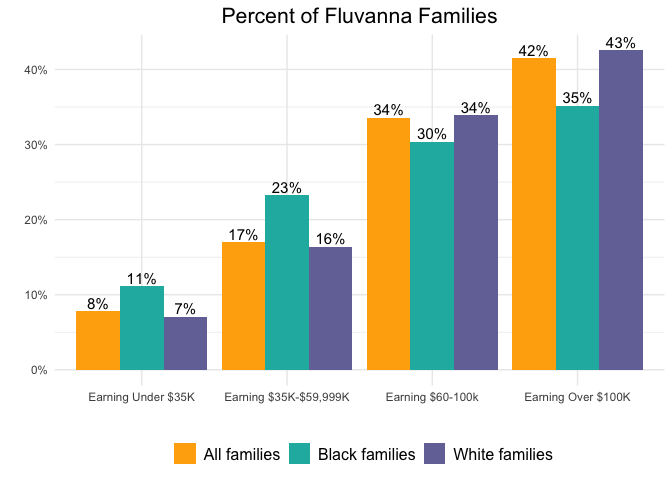
\includegraphics{orange-dot-test_files/figure-latex/unnamed-chunk-28-1} \end{center}

The maps below show the spatial relationship between income and
neighborhood. The color of each census tract in the county is based on
the median family income or the percent of families within the tract who
make less than \$35,000. Having a higher percentage of struggling
families in an area has implications for the resources and opportunities
available to the families living there.

To see which neighborhoods in Fluvanna County have the highest and
lowest median family incomes, click on each tract to see its median
income and neighborhood names.

\hypertarget{median-family-income-in-fluvanna-county}{%
\subparagraph{Median Family Income in Fluvanna
County}\label{median-family-income-in-fluvanna-county}}

The Columbia/Fork Union tract has the lowest median family incomes at
\$71,081. By contrast, the Cunningham tract has the highest median
family income at \$94,943. Relative to the other localities, the
difference between the lowest and highest values is small. On the other
hand, the highest median family income in Fluvanna is much lower than
the highest median family income in Albemarle or Charlottesville.

The following map shows the concentration of low-paid families. As in
other counties, the tract with the lowest median family income in
Fluvanna also has the highest percentage of families making less than
\$35,000 per year.

\hypertarget{percent-of-families-making-under-35000-in-fluvanna-county}{%
\subparagraph{Percent of Families Making under \$35,000 in Fluvanna
County}\label{percent-of-families-making-under-35000-in-fluvanna-county}}

\protect\hyperlink{localities}{Return to Localities ↩︎}

\hypertarget{greene-county}{%
\paragraph{Greene County}\label{greene-county}}

\hypertarget{greene-county-1}{%
\subparagraph{Greene County}\label{greene-county-1}}

There are 5,372 families living in Greene County. Of these, 791 (14.7\%)
do not earn enough to provide for their basic needs and the costs
associated with working.

Greene County at a glance:

\begin{itemize}
\item
  The costs of basic needs and working for Greene residents are around
  \$52,000, lower than the cost of expenses in Albemarle,
  Charlottesville, and Fluvanna but higher than the associated expenses
  in Nelson, Louisa, and Buckingham.
\item
  In Greene, the percent of Black families making under \$35,000 a year
  (20\%) is 18\% higher than the percent of white families making under
  \$35,000 a year (12\%).
\end{itemize}

\hypertarget{expenses-single-householder-2-children-1-toddler-4}{%
\subparagraph{Expenses: Single Householder + 2 Children (1
Toddler)}\label{expenses-single-householder-2-children-1-toddler-4}}

\global\setlength{\Oldarrayrulewidth}{\arrayrulewidth}

\global\setlength{\Oldtabcolsep}{\tabcolsep}

\setlength{\tabcolsep}{0pt}

\renewcommand*{\arraystretch}{1.5}



\providecommand{\ascline}[3]{\noalign{\global\arrayrulewidth #1}\arrayrulecolor[HTML]{#2}\cline{#3}}

\begin{longtable}[c]{|p{5.00in}|p{5.00in}|p{5.00in}|p{5.00in}}



\hhline{>{\arrayrulecolor[HTML]{666666}\global\arrayrulewidth=2pt}->{\arrayrulecolor[HTML]{666666}\global\arrayrulewidth=2pt}->{\arrayrulecolor[HTML]{666666}\global\arrayrulewidth=2pt}->{\arrayrulecolor[HTML]{666666}\global\arrayrulewidth=2pt}-}

\multicolumn{1}{>{\cellcolor[HTML]{FFFFFF}\centering}p{\dimexpr 5in+0\tabcolsep}}{\textcolor[HTML]{000000}{\fontsize{11}{11}\selectfont{Expense}}} & \multicolumn{1}{>{\cellcolor[HTML]{FFFFFF}\centering}p{\dimexpr 5in+0\tabcolsep}}{\textcolor[HTML]{000000}{\fontsize{11}{11}\selectfont{Annual}}} & \multicolumn{1}{>{\cellcolor[HTML]{FFFFFF}\centering}p{\dimexpr 5in+0\tabcolsep}}{\textcolor[HTML]{000000}{\fontsize{11}{11}\selectfont{Monthly}}} & \multicolumn{1}{>{\cellcolor[HTML]{FFFFFF}\centering}p{\dimexpr 5in+0\tabcolsep}}{\textcolor[HTML]{000000}{\fontsize{11}{11}\selectfont{Weekly}}} \\

\noalign{\global\arrayrulewidth 0pt}\arrayrulecolor[HTML]{000000}

\hhline{>{\arrayrulecolor[HTML]{666666}\global\arrayrulewidth=2pt}->{\arrayrulecolor[HTML]{666666}\global\arrayrulewidth=2pt}->{\arrayrulecolor[HTML]{666666}\global\arrayrulewidth=2pt}->{\arrayrulecolor[HTML]{666666}\global\arrayrulewidth=2pt}-}\endhead



\multicolumn{1}{>{\cellcolor[HTML]{FFFFFF}\centering}p{\dimexpr 5in+0\tabcolsep}}{\textcolor[HTML]{000000}{\fontsize{11}{11}\selectfont{Food}}} & \multicolumn{1}{>{\cellcolor[HTML]{FFFFFF}\centering}p{\dimexpr 5in+0\tabcolsep}}{\textcolor[HTML]{000000}{\fontsize{11}{11}\selectfont{6,630.0}}} & \multicolumn{1}{>{\cellcolor[HTML]{FFFFFF}\centering}p{\dimexpr 5in+0\tabcolsep}}{\textcolor[HTML]{000000}{\fontsize{11}{11}\selectfont{552.50}}} & \multicolumn{1}{>{\cellcolor[HTML]{FFFFFF}\centering}p{\dimexpr 5in+0\tabcolsep}}{\textcolor[HTML]{000000}{\fontsize{11}{11}\selectfont{127.50}}} \\

\noalign{\global\arrayrulewidth 0pt}\arrayrulecolor[HTML]{000000}

\hhline{>{\arrayrulecolor[HTML]{BEBEBE}\global\arrayrulewidth=1pt}->{\arrayrulecolor[HTML]{BEBEBE}\global\arrayrulewidth=1pt}->{\arrayrulecolor[HTML]{BEBEBE}\global\arrayrulewidth=1pt}->{\arrayrulecolor[HTML]{BEBEBE}\global\arrayrulewidth=1pt}-}



\multicolumn{1}{>{\cellcolor[HTML]{FFFFFF}\centering}p{\dimexpr 5in+0\tabcolsep}}{\textcolor[HTML]{000000}{\fontsize{11}{11}\selectfont{Clothing}}} & \multicolumn{1}{>{\cellcolor[HTML]{FFFFFF}\centering}p{\dimexpr 5in+0\tabcolsep}}{\textcolor[HTML]{000000}{\fontsize{11}{11}\selectfont{2,334.0}}} & \multicolumn{1}{>{\cellcolor[HTML]{FFFFFF}\centering}p{\dimexpr 5in+0\tabcolsep}}{\textcolor[HTML]{000000}{\fontsize{11}{11}\selectfont{194.50}}} & \multicolumn{1}{>{\cellcolor[HTML]{FFFFFF}\centering}p{\dimexpr 5in+0\tabcolsep}}{\textcolor[HTML]{000000}{\fontsize{11}{11}\selectfont{44.88}}} \\

\noalign{\global\arrayrulewidth 0pt}\arrayrulecolor[HTML]{000000}

\hhline{>{\arrayrulecolor[HTML]{BEBEBE}\global\arrayrulewidth=1pt}->{\arrayrulecolor[HTML]{BEBEBE}\global\arrayrulewidth=1pt}->{\arrayrulecolor[HTML]{BEBEBE}\global\arrayrulewidth=1pt}->{\arrayrulecolor[HTML]{BEBEBE}\global\arrayrulewidth=1pt}-}



\multicolumn{1}{>{\cellcolor[HTML]{FFFFFF}\centering}p{\dimexpr 5in+0\tabcolsep}}{\textcolor[HTML]{000000}{\fontsize{11}{11}\selectfont{Shelter}}} & \multicolumn{1}{>{\cellcolor[HTML]{FFFFFF}\centering}p{\dimexpr 5in+0\tabcolsep}}{\textcolor[HTML]{000000}{\fontsize{11}{11}\selectfont{15,168.0}}} & \multicolumn{1}{>{\cellcolor[HTML]{FFFFFF}\centering}p{\dimexpr 5in+0\tabcolsep}}{\textcolor[HTML]{000000}{\fontsize{11}{11}\selectfont{1,264.00}}} & \multicolumn{1}{>{\cellcolor[HTML]{FFFFFF}\centering}p{\dimexpr 5in+0\tabcolsep}}{\textcolor[HTML]{000000}{\fontsize{11}{11}\selectfont{291.69}}} \\

\noalign{\global\arrayrulewidth 0pt}\arrayrulecolor[HTML]{000000}

\hhline{>{\arrayrulecolor[HTML]{BEBEBE}\global\arrayrulewidth=1pt}->{\arrayrulecolor[HTML]{BEBEBE}\global\arrayrulewidth=1pt}->{\arrayrulecolor[HTML]{BEBEBE}\global\arrayrulewidth=1pt}->{\arrayrulecolor[HTML]{BEBEBE}\global\arrayrulewidth=1pt}-}



\multicolumn{1}{>{\cellcolor[HTML]{FFFFFF}\centering}p{\dimexpr 5in+0\tabcolsep}}{\textcolor[HTML]{000000}{\fontsize{11}{11}\selectfont{Utilities}}} & \multicolumn{1}{>{\cellcolor[HTML]{FFFFFF}\centering}p{\dimexpr 5in+0\tabcolsep}}{\textcolor[HTML]{000000}{\fontsize{11}{11}\selectfont{3,325.0}}} & \multicolumn{1}{>{\cellcolor[HTML]{FFFFFF}\centering}p{\dimexpr 5in+0\tabcolsep}}{\textcolor[HTML]{000000}{\fontsize{11}{11}\selectfont{277.08}}} & \multicolumn{1}{>{\cellcolor[HTML]{FFFFFF}\centering}p{\dimexpr 5in+0\tabcolsep}}{\textcolor[HTML]{000000}{\fontsize{11}{11}\selectfont{63.94}}} \\

\noalign{\global\arrayrulewidth 0pt}\arrayrulecolor[HTML]{000000}

\hhline{>{\arrayrulecolor[HTML]{BEBEBE}\global\arrayrulewidth=1pt}->{\arrayrulecolor[HTML]{BEBEBE}\global\arrayrulewidth=1pt}->{\arrayrulecolor[HTML]{BEBEBE}\global\arrayrulewidth=1pt}->{\arrayrulecolor[HTML]{BEBEBE}\global\arrayrulewidth=1pt}-}



\multicolumn{1}{>{\cellcolor[HTML]{FFFFFF}\centering}p{\dimexpr 5in+0\tabcolsep}}{\textcolor[HTML]{000000}{\fontsize{11}{11}\selectfont{Necessary\ Costs}}} & \multicolumn{1}{>{\cellcolor[HTML]{FFFFFF}\centering}p{\dimexpr 5in+0\tabcolsep}}{\textcolor[HTML]{000000}{\fontsize{11}{11}\selectfont{5,491.4}}} & \multicolumn{1}{>{\cellcolor[HTML]{FFFFFF}\centering}p{\dimexpr 5in+0\tabcolsep}}{\textcolor[HTML]{000000}{\fontsize{11}{11}\selectfont{457.62}}} & \multicolumn{1}{>{\cellcolor[HTML]{FFFFFF}\centering}p{\dimexpr 5in+0\tabcolsep}}{\textcolor[HTML]{000000}{\fontsize{11}{11}\selectfont{105.60}}} \\

\noalign{\global\arrayrulewidth 0pt}\arrayrulecolor[HTML]{000000}

\hhline{>{\arrayrulecolor[HTML]{BEBEBE}\global\arrayrulewidth=1pt}->{\arrayrulecolor[HTML]{BEBEBE}\global\arrayrulewidth=1pt}->{\arrayrulecolor[HTML]{BEBEBE}\global\arrayrulewidth=1pt}->{\arrayrulecolor[HTML]{BEBEBE}\global\arrayrulewidth=1pt}-}



\multicolumn{1}{>{\cellcolor[HTML]{FFAD0A}\centering}p{\dimexpr 5in+0\tabcolsep}}{\textcolor[HTML]{000000}{\fontsize{11}{11}\selectfont{Survival\ Expenses}}} & \multicolumn{1}{>{\cellcolor[HTML]{FFAD0A}\centering}p{\dimexpr 5in+0\tabcolsep}}{\textcolor[HTML]{000000}{\fontsize{11}{11}\selectfont{32,948.4}}} & \multicolumn{1}{>{\cellcolor[HTML]{FFAD0A}\centering}p{\dimexpr 5in+0\tabcolsep}}{\textcolor[HTML]{000000}{\fontsize{11}{11}\selectfont{2,745.70}}} & \multicolumn{1}{>{\cellcolor[HTML]{FFAD0A}\centering}p{\dimexpr 5in+0\tabcolsep}}{\textcolor[HTML]{000000}{\fontsize{11}{11}\selectfont{633.62}}} \\

\noalign{\global\arrayrulewidth 0pt}\arrayrulecolor[HTML]{000000}

\hhline{>{\arrayrulecolor[HTML]{BEBEBE}\global\arrayrulewidth=1pt}->{\arrayrulecolor[HTML]{BEBEBE}\global\arrayrulewidth=1pt}->{\arrayrulecolor[HTML]{BEBEBE}\global\arrayrulewidth=1pt}->{\arrayrulecolor[HTML]{BEBEBE}\global\arrayrulewidth=1pt}-}



\multicolumn{1}{>{\cellcolor[HTML]{FFFFFF}\centering}p{\dimexpr 5in+0\tabcolsep}}{\textcolor[HTML]{000000}{\fontsize{11}{11}\selectfont{Childcare}}} & \multicolumn{1}{>{\cellcolor[HTML]{FFFFFF}\centering}p{\dimexpr 5in+0\tabcolsep}}{\textcolor[HTML]{000000}{\fontsize{11}{11}\selectfont{14,300.0}}} & \multicolumn{1}{>{\cellcolor[HTML]{FFFFFF}\centering}p{\dimexpr 5in+0\tabcolsep}}{\textcolor[HTML]{000000}{\fontsize{11}{11}\selectfont{1,192.00}}} & \multicolumn{1}{>{\cellcolor[HTML]{FFFFFF}\centering}p{\dimexpr 5in+0\tabcolsep}}{\textcolor[HTML]{000000}{\fontsize{11}{11}\selectfont{275.00}}} \\

\noalign{\global\arrayrulewidth 0pt}\arrayrulecolor[HTML]{000000}

\hhline{>{\arrayrulecolor[HTML]{BEBEBE}\global\arrayrulewidth=1pt}->{\arrayrulecolor[HTML]{BEBEBE}\global\arrayrulewidth=1pt}->{\arrayrulecolor[HTML]{BEBEBE}\global\arrayrulewidth=1pt}->{\arrayrulecolor[HTML]{BEBEBE}\global\arrayrulewidth=1pt}-}



\multicolumn{1}{>{\cellcolor[HTML]{FFFFFF}\centering}p{\dimexpr 5in+0\tabcolsep}}{\textcolor[HTML]{000000}{\fontsize{11}{11}\selectfont{Transportation}}} & \multicolumn{1}{>{\cellcolor[HTML]{FFFFFF}\centering}p{\dimexpr 5in+0\tabcolsep}}{\textcolor[HTML]{000000}{\fontsize{11}{11}\selectfont{3,996.0}}} & \multicolumn{1}{>{\cellcolor[HTML]{FFFFFF}\centering}p{\dimexpr 5in+0\tabcolsep}}{\textcolor[HTML]{000000}{\fontsize{11}{11}\selectfont{333.00}}} & \multicolumn{1}{>{\cellcolor[HTML]{FFFFFF}\centering}p{\dimexpr 5in+0\tabcolsep}}{\textcolor[HTML]{000000}{\fontsize{11}{11}\selectfont{76.85}}} \\

\noalign{\global\arrayrulewidth 0pt}\arrayrulecolor[HTML]{000000}

\hhline{>{\arrayrulecolor[HTML]{BEBEBE}\global\arrayrulewidth=1pt}->{\arrayrulecolor[HTML]{BEBEBE}\global\arrayrulewidth=1pt}->{\arrayrulecolor[HTML]{BEBEBE}\global\arrayrulewidth=1pt}->{\arrayrulecolor[HTML]{BEBEBE}\global\arrayrulewidth=1pt}-}



\multicolumn{1}{>{\cellcolor[HTML]{EE6100}\centering}p{\dimexpr 5in+0\tabcolsep}}{\textcolor[HTML]{FFFFFF}{\fontsize{11}{11}\selectfont{Total\ Expenses}}} & \multicolumn{1}{>{\cellcolor[HTML]{EE6100}\centering}p{\dimexpr 5in+0\tabcolsep}}{\textcolor[HTML]{FFFFFF}{\fontsize{11}{11}\selectfont{51,244.4}}} & \multicolumn{1}{>{\cellcolor[HTML]{EE6100}\centering}p{\dimexpr 5in+0\tabcolsep}}{\textcolor[HTML]{FFFFFF}{\fontsize{11}{11}\selectfont{4,116.20}}} & \multicolumn{1}{>{\cellcolor[HTML]{EE6100}\centering}p{\dimexpr 5in+0\tabcolsep}}{\textcolor[HTML]{FFFFFF}{\fontsize{11}{11}\selectfont{949.89}}} \\

\noalign{\global\arrayrulewidth 0pt}\arrayrulecolor[HTML]{000000}

\hhline{>{\arrayrulecolor[HTML]{666666}\global\arrayrulewidth=2pt}->{\arrayrulecolor[HTML]{666666}\global\arrayrulewidth=2pt}->{\arrayrulecolor[HTML]{666666}\global\arrayrulewidth=2pt}->{\arrayrulecolor[HTML]{666666}\global\arrayrulewidth=2pt}-}



\end{longtable}



\arrayrulecolor[HTML]{000000}

\global\setlength{\arrayrulewidth}{\Oldarrayrulewidth}

\global\setlength{\tabcolsep}{\Oldtabcolsep}

\renewcommand*{\arraystretch}{1}

\hypertarget{breakdown-of-families-making-under-35000-in-greene-county}{%
\subparagraph{Breakdown of Families Making under \$35,000 in Greene
County}\label{breakdown-of-families-making-under-35000-in-greene-county}}

\global\setlength{\Oldarrayrulewidth}{\arrayrulewidth}

\global\setlength{\Oldtabcolsep}{\tabcolsep}

\setlength{\tabcolsep}{0pt}

\renewcommand*{\arraystretch}{1.5}



\providecommand{\ascline}[3]{\noalign{\global\arrayrulewidth #1}\arrayrulecolor[HTML]{#2}\cline{#3}}

\begin{longtable}[c]{|p{5.00in}|p{5.00in}|p{5.00in}|p{5.00in}}



\hhline{>{\arrayrulecolor[HTML]{666666}\global\arrayrulewidth=2pt}->{\arrayrulecolor[HTML]{666666}\global\arrayrulewidth=2pt}->{\arrayrulecolor[HTML]{666666}\global\arrayrulewidth=2pt}->{\arrayrulecolor[HTML]{666666}\global\arrayrulewidth=2pt}-}

\multicolumn{1}{>{\cellcolor[HTML]{FFFFFF}\centering}p{\dimexpr 5in+0\tabcolsep}}{\textcolor[HTML]{000000}{\fontsize{11}{11}\selectfont{Income}}} & \multicolumn{1}{>{\cellcolor[HTML]{FFFFFF}\centering}p{\dimexpr 5in+0\tabcolsep}}{\textcolor[HTML]{000000}{\fontsize{11}{11}\selectfont{Number}}} & \multicolumn{1}{>{\cellcolor[HTML]{FFFFFF}\centering}p{\dimexpr 5in+0\tabcolsep}}{\textcolor[HTML]{000000}{\fontsize{11}{11}\selectfont{Percent}}} & \multicolumn{1}{>{\cellcolor[HTML]{FFFFFF}\centering}p{\dimexpr 5in+0\tabcolsep}}{\textcolor[HTML]{000000}{\fontsize{11}{11}\selectfont{Cumulative}}} \\

\noalign{\global\arrayrulewidth 0pt}\arrayrulecolor[HTML]{000000}

\hhline{>{\arrayrulecolor[HTML]{666666}\global\arrayrulewidth=2pt}->{\arrayrulecolor[HTML]{666666}\global\arrayrulewidth=2pt}->{\arrayrulecolor[HTML]{666666}\global\arrayrulewidth=2pt}->{\arrayrulecolor[HTML]{666666}\global\arrayrulewidth=2pt}-}\endhead



\multicolumn{1}{>{\cellcolor[HTML]{FFFFFF}\centering}p{\dimexpr 5in+0\tabcolsep}}{\textcolor[HTML]{000000}{\fontsize{11}{11}\selectfont{\$0\ -\ \$9,999}}} & \multicolumn{1}{>{\cellcolor[HTML]{FFFFFF}\centering}p{\dimexpr 5in+0\tabcolsep}}{\textcolor[HTML]{000000}{\fontsize{11}{11}\selectfont{58}}} & \multicolumn{1}{>{\cellcolor[HTML]{FFFFFF}\centering}p{\dimexpr 5in+0\tabcolsep}}{\textcolor[HTML]{000000}{\fontsize{11}{11}\selectfont{7\%}}} & \multicolumn{1}{>{\cellcolor[HTML]{FFAD0A}\centering}p{\dimexpr 5in+0\tabcolsep}}{} \\

\noalign{\global\arrayrulewidth 0pt}\arrayrulecolor[HTML]{000000}

\hhline{>{\arrayrulecolor[HTML]{BEBEBE}\global\arrayrulewidth=1pt}->{\arrayrulecolor[HTML]{BEBEBE}\global\arrayrulewidth=1pt}->{\arrayrulecolor[HTML]{BEBEBE}\global\arrayrulewidth=1pt}->{\arrayrulecolor[HTML]{FFAD0A}\global\arrayrulewidth=1pt}-}



\multicolumn{1}{>{\cellcolor[HTML]{FFFFFF}\centering}p{\dimexpr 5in+0\tabcolsep}}{\textcolor[HTML]{000000}{\fontsize{11}{11}\selectfont{\$10,000\ -\ \$14,999}}} & \multicolumn{1}{>{\cellcolor[HTML]{FFFFFF}\centering}p{\dimexpr 5in+0\tabcolsep}}{\textcolor[HTML]{000000}{\fontsize{11}{11}\selectfont{119}}} & \multicolumn{1}{>{\cellcolor[HTML]{FFFFFF}\centering}p{\dimexpr 5in+0\tabcolsep}}{\textcolor[HTML]{000000}{\fontsize{11}{11}\selectfont{15\%}}} & \multicolumn{1}{>{\cellcolor[HTML]{FFAD0A}\centering}p{\dimexpr 5in+0\tabcolsep}}{\multirow[c]{-2}{*}{\parbox{5in}{\textcolor[HTML]{000000}{\fontsize{11}{11}\selectfont{22\%}}}}} \\

\noalign{\global\arrayrulewidth 0pt}\arrayrulecolor[HTML]{000000}

\hhline{>{\arrayrulecolor[HTML]{BEBEBE}\global\arrayrulewidth=1pt}->{\arrayrulecolor[HTML]{BEBEBE}\global\arrayrulewidth=1pt}->{\arrayrulecolor[HTML]{BEBEBE}\global\arrayrulewidth=1pt}->{\arrayrulecolor[HTML]{BEBEBE}\global\arrayrulewidth=1pt}-}



\multicolumn{1}{>{\cellcolor[HTML]{FFFFFF}\centering}p{\dimexpr 5in+0\tabcolsep}}{\textcolor[HTML]{000000}{\fontsize{11}{11}\selectfont{\$15,000\ -\ \$24,999}}} & \multicolumn{1}{>{\cellcolor[HTML]{FFFFFF}\centering}p{\dimexpr 5in+0\tabcolsep}}{\textcolor[HTML]{000000}{\fontsize{11}{11}\selectfont{291}}} & \multicolumn{1}{>{\cellcolor[HTML]{FFFFFF}\centering}p{\dimexpr 5in+0\tabcolsep}}{\textcolor[HTML]{000000}{\fontsize{11}{11}\selectfont{37\%}}} & \multicolumn{1}{>{\cellcolor[HTML]{EE6100}\centering}p{\dimexpr 5in+0\tabcolsep}}{} \\

\noalign{\global\arrayrulewidth 0pt}\arrayrulecolor[HTML]{000000}

\hhline{>{\arrayrulecolor[HTML]{BEBEBE}\global\arrayrulewidth=1pt}->{\arrayrulecolor[HTML]{BEBEBE}\global\arrayrulewidth=1pt}->{\arrayrulecolor[HTML]{BEBEBE}\global\arrayrulewidth=1pt}->{\arrayrulecolor[HTML]{EE6100}\global\arrayrulewidth=1pt}-}



\multicolumn{1}{>{\cellcolor[HTML]{FFFFFF}\centering}p{\dimexpr 5in+0\tabcolsep}}{\textcolor[HTML]{000000}{\fontsize{11}{11}\selectfont{\$25,000\ -\ \$34,999}}} & \multicolumn{1}{>{\cellcolor[HTML]{FFFFFF}\centering}p{\dimexpr 5in+0\tabcolsep}}{\textcolor[HTML]{000000}{\fontsize{11}{11}\selectfont{323}}} & \multicolumn{1}{>{\cellcolor[HTML]{FFFFFF}\centering}p{\dimexpr 5in+0\tabcolsep}}{\textcolor[HTML]{000000}{\fontsize{11}{11}\selectfont{41\%}}} & \multicolumn{1}{>{\cellcolor[HTML]{EE6100}\centering}p{\dimexpr 5in+0\tabcolsep}}{\multirow[c]{-2}{*}{\parbox{5in}{\textcolor[HTML]{FFFFFF}{\fontsize{11}{11}\selectfont{78\%}}}}} \\

\noalign{\global\arrayrulewidth 0pt}\arrayrulecolor[HTML]{000000}

\hhline{>{\arrayrulecolor[HTML]{BEBEBE}\global\arrayrulewidth=1pt}->{\arrayrulecolor[HTML]{BEBEBE}\global\arrayrulewidth=1pt}->{\arrayrulecolor[HTML]{BEBEBE}\global\arrayrulewidth=1pt}->{\arrayrulecolor[HTML]{BEBEBE}\global\arrayrulewidth=1pt}-}



\multicolumn{1}{>{\cellcolor[HTML]{FFFFFF}\centering}p{\dimexpr 5in+0\tabcolsep}}{\textcolor[HTML]{000000}{\fontsize{11}{11}\selectfont{Total}}} & \multicolumn{1}{>{\cellcolor[HTML]{FFFFFF}\centering}p{\dimexpr 5in+0\tabcolsep}}{\textcolor[HTML]{000000}{\fontsize{11}{11}\selectfont{791}}} & \multicolumn{2}{>{\cellcolor[HTML]{FFFFFF}\centering}p{\dimexpr 10in+2\tabcolsep}}{\textcolor[HTML]{000000}{\fontsize{11}{11}\selectfont{100\%}}} \\

\noalign{\global\arrayrulewidth 0pt}\arrayrulecolor[HTML]{000000}

\hhline{>{\arrayrulecolor[HTML]{666666}\global\arrayrulewidth=2pt}->{\arrayrulecolor[HTML]{666666}\global\arrayrulewidth=2pt}->{\arrayrulecolor[HTML]{666666}\global\arrayrulewidth=2pt}->{\arrayrulecolor[HTML]{666666}\global\arrayrulewidth=2pt}-}



\end{longtable}



\arrayrulecolor[HTML]{000000}

\global\setlength{\arrayrulewidth}{\Oldarrayrulewidth}

\global\setlength{\tabcolsep}{\Oldtabcolsep}

\renewcommand*{\arraystretch}{1}

As this table shows, 78\% of the families who cannot meet their basic
needs earn between \$15,000-\$35,000 annually. This strongly suggests
they are working, but not earning the wages or not getting the hours
they need to support their families.

The figure below shows the distribution of families in various pay
ranges, disaggregated by race. In a world with racial equity in income,
the bars for all families would be equal in height. In Greene County,
Black families are very over-represented at the low end of the pay range
(under \$35,000) and slightly under-represented at the high end of the
pay range (over \$100,000). In other words, relative to white families,
Black families are more likely to be paid insufficient wages.

\hypertarget{income-distribution-of-black-and-white-families-in-greene-county}{%
\subparagraph{Income Distribution of Black and White Families in Greene
County}\label{income-distribution-of-black-and-white-families-in-greene-county}}

\begin{center}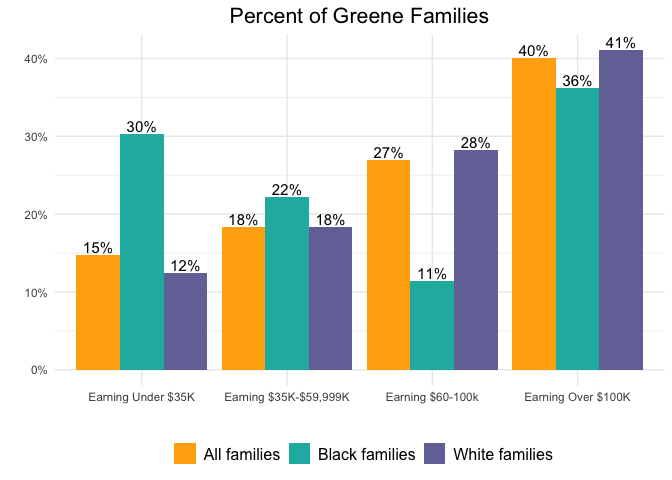
\includegraphics{orange-dot-test_files/figure-latex/unnamed-chunk-34-1} \end{center}

The maps below show the spatial relationship between income and
neighborhood. The color of each census tract in the county is based on
the median family income or the percent of families within the tract who
make less than \$35,000 yearly.

To see which neighborhoods in Greene County have the highest and lowest
median family incomes, click on each tract to see its median income and
neighborhood names.

\hypertarget{median-family-income-in-greene-county}{%
\subparagraph{Median Family Income in Greene
County}\label{median-family-income-in-greene-county}}

The Stanardsville tract has the lowest median family incomes at
\$61,930. By contrast, the Midway tract has the highest median family
income at \$103,679.

The following map shows the concentration of low-paid families. Similar
to the other counties, in Greene County, the tract with the lowest
median family income also has the highest percentage of families making
less than \$35,000.

\hypertarget{percent-of-families-making-under-35000-in-greene-county}{%
\subparagraph{Percent of Families Making under \$35,000 in Greene
County}\label{percent-of-families-making-under-35000-in-greene-county}}

\protect\hyperlink{localities}{Return to Localities ↩︎}

\hypertarget{louisa-county}{%
\paragraph{Louisa County}\label{louisa-county}}

\hypertarget{louisa-county-1}{%
\subparagraph{Louisa County}\label{louisa-county-1}}

There are 10,249 families living in Louisa County. Of these, 1,791
(17.5\%) do not earn enough to provide for their basic needs and the
costs associated with working.

Louisa at a glance:

\begin{itemize}
\item
  Louisa has the second highest number of families falling behind: 19\%
  of the 9,413 families struggling in our region live in Louisa.
\item
  Louisa has one of the lowest costs for basic needs and the cost of
  working, at \$45,917, second only to Buckingham.
\item
  In Louisa, the percent of Black families making under \$35,000 (26\%)
  is 11\% higher than the percent of white families making under
  \$35,000 (15\%).
\end{itemize}

\hypertarget{expenses-single-householder-2-children-1-toddler-5}{%
\subparagraph{Expenses: Single Householder + 2 Children (1
Toddler)}\label{expenses-single-householder-2-children-1-toddler-5}}

\global\setlength{\Oldarrayrulewidth}{\arrayrulewidth}

\global\setlength{\Oldtabcolsep}{\tabcolsep}

\setlength{\tabcolsep}{0pt}

\renewcommand*{\arraystretch}{1.5}



\providecommand{\ascline}[3]{\noalign{\global\arrayrulewidth #1}\arrayrulecolor[HTML]{#2}\cline{#3}}

\begin{longtable}[c]{|p{5.00in}|p{5.00in}|p{5.00in}|p{5.00in}}



\hhline{>{\arrayrulecolor[HTML]{666666}\global\arrayrulewidth=2pt}->{\arrayrulecolor[HTML]{666666}\global\arrayrulewidth=2pt}->{\arrayrulecolor[HTML]{666666}\global\arrayrulewidth=2pt}->{\arrayrulecolor[HTML]{666666}\global\arrayrulewidth=2pt}-}

\multicolumn{1}{>{\cellcolor[HTML]{FFFFFF}\centering}p{\dimexpr 5in+0\tabcolsep}}{\textcolor[HTML]{000000}{\fontsize{11}{11}\selectfont{Expense}}} & \multicolumn{1}{>{\cellcolor[HTML]{FFFFFF}\centering}p{\dimexpr 5in+0\tabcolsep}}{\textcolor[HTML]{000000}{\fontsize{11}{11}\selectfont{Annual}}} & \multicolumn{1}{>{\cellcolor[HTML]{FFFFFF}\centering}p{\dimexpr 5in+0\tabcolsep}}{\textcolor[HTML]{000000}{\fontsize{11}{11}\selectfont{Monthly}}} & \multicolumn{1}{>{\cellcolor[HTML]{FFFFFF}\centering}p{\dimexpr 5in+0\tabcolsep}}{\textcolor[HTML]{000000}{\fontsize{11}{11}\selectfont{Weekly}}} \\

\noalign{\global\arrayrulewidth 0pt}\arrayrulecolor[HTML]{000000}

\hhline{>{\arrayrulecolor[HTML]{666666}\global\arrayrulewidth=2pt}->{\arrayrulecolor[HTML]{666666}\global\arrayrulewidth=2pt}->{\arrayrulecolor[HTML]{666666}\global\arrayrulewidth=2pt}->{\arrayrulecolor[HTML]{666666}\global\arrayrulewidth=2pt}-}\endhead



\multicolumn{1}{>{\cellcolor[HTML]{FFFFFF}\centering}p{\dimexpr 5in+0\tabcolsep}}{\textcolor[HTML]{000000}{\fontsize{11}{11}\selectfont{Food}}} & \multicolumn{1}{>{\cellcolor[HTML]{FFFFFF}\centering}p{\dimexpr 5in+0\tabcolsep}}{\textcolor[HTML]{000000}{\fontsize{11}{11}\selectfont{6,630.0}}} & \multicolumn{1}{>{\cellcolor[HTML]{FFFFFF}\centering}p{\dimexpr 5in+0\tabcolsep}}{\textcolor[HTML]{000000}{\fontsize{11}{11}\selectfont{552.50}}} & \multicolumn{1}{>{\cellcolor[HTML]{FFFFFF}\centering}p{\dimexpr 5in+0\tabcolsep}}{\textcolor[HTML]{000000}{\fontsize{11}{11}\selectfont{127.50}}} \\

\noalign{\global\arrayrulewidth 0pt}\arrayrulecolor[HTML]{000000}

\hhline{>{\arrayrulecolor[HTML]{BEBEBE}\global\arrayrulewidth=1pt}->{\arrayrulecolor[HTML]{BEBEBE}\global\arrayrulewidth=1pt}->{\arrayrulecolor[HTML]{BEBEBE}\global\arrayrulewidth=1pt}->{\arrayrulecolor[HTML]{BEBEBE}\global\arrayrulewidth=1pt}-}



\multicolumn{1}{>{\cellcolor[HTML]{FFFFFF}\centering}p{\dimexpr 5in+0\tabcolsep}}{\textcolor[HTML]{000000}{\fontsize{11}{11}\selectfont{Clothing}}} & \multicolumn{1}{>{\cellcolor[HTML]{FFFFFF}\centering}p{\dimexpr 5in+0\tabcolsep}}{\textcolor[HTML]{000000}{\fontsize{11}{11}\selectfont{2,334.0}}} & \multicolumn{1}{>{\cellcolor[HTML]{FFFFFF}\centering}p{\dimexpr 5in+0\tabcolsep}}{\textcolor[HTML]{000000}{\fontsize{11}{11}\selectfont{194.50}}} & \multicolumn{1}{>{\cellcolor[HTML]{FFFFFF}\centering}p{\dimexpr 5in+0\tabcolsep}}{\textcolor[HTML]{000000}{\fontsize{11}{11}\selectfont{44.88}}} \\

\noalign{\global\arrayrulewidth 0pt}\arrayrulecolor[HTML]{000000}

\hhline{>{\arrayrulecolor[HTML]{BEBEBE}\global\arrayrulewidth=1pt}->{\arrayrulecolor[HTML]{BEBEBE}\global\arrayrulewidth=1pt}->{\arrayrulecolor[HTML]{BEBEBE}\global\arrayrulewidth=1pt}->{\arrayrulecolor[HTML]{BEBEBE}\global\arrayrulewidth=1pt}-}



\multicolumn{1}{>{\cellcolor[HTML]{FFFFFF}\centering}p{\dimexpr 5in+0\tabcolsep}}{\textcolor[HTML]{000000}{\fontsize{11}{11}\selectfont{Shelter}}} & \multicolumn{1}{>{\cellcolor[HTML]{FFFFFF}\centering}p{\dimexpr 5in+0\tabcolsep}}{\textcolor[HTML]{000000}{\fontsize{11}{11}\selectfont{10,512.0}}} & \multicolumn{1}{>{\cellcolor[HTML]{FFFFFF}\centering}p{\dimexpr 5in+0\tabcolsep}}{\textcolor[HTML]{000000}{\fontsize{11}{11}\selectfont{876.00}}} & \multicolumn{1}{>{\cellcolor[HTML]{FFFFFF}\centering}p{\dimexpr 5in+0\tabcolsep}}{\textcolor[HTML]{000000}{\fontsize{11}{11}\selectfont{202.15}}} \\

\noalign{\global\arrayrulewidth 0pt}\arrayrulecolor[HTML]{000000}

\hhline{>{\arrayrulecolor[HTML]{BEBEBE}\global\arrayrulewidth=1pt}->{\arrayrulecolor[HTML]{BEBEBE}\global\arrayrulewidth=1pt}->{\arrayrulecolor[HTML]{BEBEBE}\global\arrayrulewidth=1pt}->{\arrayrulecolor[HTML]{BEBEBE}\global\arrayrulewidth=1pt}-}



\multicolumn{1}{>{\cellcolor[HTML]{FFFFFF}\centering}p{\dimexpr 5in+0\tabcolsep}}{\textcolor[HTML]{000000}{\fontsize{11}{11}\selectfont{Utilities}}} & \multicolumn{1}{>{\cellcolor[HTML]{FFFFFF}\centering}p{\dimexpr 5in+0\tabcolsep}}{\textcolor[HTML]{000000}{\fontsize{11}{11}\selectfont{3,325.0}}} & \multicolumn{1}{>{\cellcolor[HTML]{FFFFFF}\centering}p{\dimexpr 5in+0\tabcolsep}}{\textcolor[HTML]{000000}{\fontsize{11}{11}\selectfont{277.08}}} & \multicolumn{1}{>{\cellcolor[HTML]{FFFFFF}\centering}p{\dimexpr 5in+0\tabcolsep}}{\textcolor[HTML]{000000}{\fontsize{11}{11}\selectfont{63.94}}} \\

\noalign{\global\arrayrulewidth 0pt}\arrayrulecolor[HTML]{000000}

\hhline{>{\arrayrulecolor[HTML]{BEBEBE}\global\arrayrulewidth=1pt}->{\arrayrulecolor[HTML]{BEBEBE}\global\arrayrulewidth=1pt}->{\arrayrulecolor[HTML]{BEBEBE}\global\arrayrulewidth=1pt}->{\arrayrulecolor[HTML]{BEBEBE}\global\arrayrulewidth=1pt}-}



\multicolumn{1}{>{\cellcolor[HTML]{FFFFFF}\centering}p{\dimexpr 5in+0\tabcolsep}}{\textcolor[HTML]{000000}{\fontsize{11}{11}\selectfont{Necessary\ Costs}}} & \multicolumn{1}{>{\cellcolor[HTML]{FFFFFF}\centering}p{\dimexpr 5in+0\tabcolsep}}{\textcolor[HTML]{000000}{\fontsize{11}{11}\selectfont{4,560.2}}} & \multicolumn{1}{>{\cellcolor[HTML]{FFFFFF}\centering}p{\dimexpr 5in+0\tabcolsep}}{\textcolor[HTML]{000000}{\fontsize{11}{11}\selectfont{380.02}}} & \multicolumn{1}{>{\cellcolor[HTML]{FFFFFF}\centering}p{\dimexpr 5in+0\tabcolsep}}{\textcolor[HTML]{000000}{\fontsize{11}{11}\selectfont{87.70}}} \\

\noalign{\global\arrayrulewidth 0pt}\arrayrulecolor[HTML]{000000}

\hhline{>{\arrayrulecolor[HTML]{BEBEBE}\global\arrayrulewidth=1pt}->{\arrayrulecolor[HTML]{BEBEBE}\global\arrayrulewidth=1pt}->{\arrayrulecolor[HTML]{BEBEBE}\global\arrayrulewidth=1pt}->{\arrayrulecolor[HTML]{BEBEBE}\global\arrayrulewidth=1pt}-}



\multicolumn{1}{>{\cellcolor[HTML]{FFAD0A}\centering}p{\dimexpr 5in+0\tabcolsep}}{\textcolor[HTML]{000000}{\fontsize{11}{11}\selectfont{Survival\ Expenses}}} & \multicolumn{1}{>{\cellcolor[HTML]{FFAD0A}\centering}p{\dimexpr 5in+0\tabcolsep}}{\textcolor[HTML]{000000}{\fontsize{11}{11}\selectfont{27,361.2}}} & \multicolumn{1}{>{\cellcolor[HTML]{FFAD0A}\centering}p{\dimexpr 5in+0\tabcolsep}}{\textcolor[HTML]{000000}{\fontsize{11}{11}\selectfont{2,280.10}}} & \multicolumn{1}{>{\cellcolor[HTML]{FFAD0A}\centering}p{\dimexpr 5in+0\tabcolsep}}{\textcolor[HTML]{000000}{\fontsize{11}{11}\selectfont{526.18}}} \\

\noalign{\global\arrayrulewidth 0pt}\arrayrulecolor[HTML]{000000}

\hhline{>{\arrayrulecolor[HTML]{BEBEBE}\global\arrayrulewidth=1pt}->{\arrayrulecolor[HTML]{BEBEBE}\global\arrayrulewidth=1pt}->{\arrayrulecolor[HTML]{BEBEBE}\global\arrayrulewidth=1pt}->{\arrayrulecolor[HTML]{BEBEBE}\global\arrayrulewidth=1pt}-}



\multicolumn{1}{>{\cellcolor[HTML]{FFFFFF}\centering}p{\dimexpr 5in+0\tabcolsep}}{\textcolor[HTML]{000000}{\fontsize{11}{11}\selectfont{Childcare}}} & \multicolumn{1}{>{\cellcolor[HTML]{FFFFFF}\centering}p{\dimexpr 5in+0\tabcolsep}}{\textcolor[HTML]{000000}{\fontsize{11}{11}\selectfont{14,560.0}}} & \multicolumn{1}{>{\cellcolor[HTML]{FFFFFF}\centering}p{\dimexpr 5in+0\tabcolsep}}{\textcolor[HTML]{000000}{\fontsize{11}{11}\selectfont{1,213.00}}} & \multicolumn{1}{>{\cellcolor[HTML]{FFFFFF}\centering}p{\dimexpr 5in+0\tabcolsep}}{\textcolor[HTML]{000000}{\fontsize{11}{11}\selectfont{280.00}}} \\

\noalign{\global\arrayrulewidth 0pt}\arrayrulecolor[HTML]{000000}

\hhline{>{\arrayrulecolor[HTML]{BEBEBE}\global\arrayrulewidth=1pt}->{\arrayrulecolor[HTML]{BEBEBE}\global\arrayrulewidth=1pt}->{\arrayrulecolor[HTML]{BEBEBE}\global\arrayrulewidth=1pt}->{\arrayrulecolor[HTML]{BEBEBE}\global\arrayrulewidth=1pt}-}



\multicolumn{1}{>{\cellcolor[HTML]{FFFFFF}\centering}p{\dimexpr 5in+0\tabcolsep}}{\textcolor[HTML]{000000}{\fontsize{11}{11}\selectfont{Transportation}}} & \multicolumn{1}{>{\cellcolor[HTML]{FFFFFF}\centering}p{\dimexpr 5in+0\tabcolsep}}{\textcolor[HTML]{000000}{\fontsize{11}{11}\selectfont{3,996.0}}} & \multicolumn{1}{>{\cellcolor[HTML]{FFFFFF}\centering}p{\dimexpr 5in+0\tabcolsep}}{\textcolor[HTML]{000000}{\fontsize{11}{11}\selectfont{333.00}}} & \multicolumn{1}{>{\cellcolor[HTML]{FFFFFF}\centering}p{\dimexpr 5in+0\tabcolsep}}{\textcolor[HTML]{000000}{\fontsize{11}{11}\selectfont{76.85}}} \\

\noalign{\global\arrayrulewidth 0pt}\arrayrulecolor[HTML]{000000}

\hhline{>{\arrayrulecolor[HTML]{BEBEBE}\global\arrayrulewidth=1pt}->{\arrayrulecolor[HTML]{BEBEBE}\global\arrayrulewidth=1pt}->{\arrayrulecolor[HTML]{BEBEBE}\global\arrayrulewidth=1pt}->{\arrayrulecolor[HTML]{BEBEBE}\global\arrayrulewidth=1pt}-}



\multicolumn{1}{>{\cellcolor[HTML]{EE6100}\centering}p{\dimexpr 5in+0\tabcolsep}}{\textcolor[HTML]{FFFFFF}{\fontsize{11}{11}\selectfont{Total\ Expenses}}} & \multicolumn{1}{>{\cellcolor[HTML]{EE6100}\centering}p{\dimexpr 5in+0\tabcolsep}}{\textcolor[HTML]{FFFFFF}{\fontsize{11}{11}\selectfont{45,917.2}}} & \multicolumn{1}{>{\cellcolor[HTML]{EE6100}\centering}p{\dimexpr 5in+0\tabcolsep}}{\textcolor[HTML]{FFFFFF}{\fontsize{11}{11}\selectfont{3,650.60}}} & \multicolumn{1}{>{\cellcolor[HTML]{EE6100}\centering}p{\dimexpr 5in+0\tabcolsep}}{\textcolor[HTML]{FFFFFF}{\fontsize{11}{11}\selectfont{842.45}}} \\

\noalign{\global\arrayrulewidth 0pt}\arrayrulecolor[HTML]{000000}

\hhline{>{\arrayrulecolor[HTML]{666666}\global\arrayrulewidth=2pt}->{\arrayrulecolor[HTML]{666666}\global\arrayrulewidth=2pt}->{\arrayrulecolor[HTML]{666666}\global\arrayrulewidth=2pt}->{\arrayrulecolor[HTML]{666666}\global\arrayrulewidth=2pt}-}



\end{longtable}



\arrayrulecolor[HTML]{000000}

\global\setlength{\arrayrulewidth}{\Oldarrayrulewidth}

\global\setlength{\tabcolsep}{\Oldtabcolsep}

\renewcommand*{\arraystretch}{1}

\hypertarget{breakdown-of-families-making-under-35000-in-louisa-county}{%
\subparagraph{Breakdown of Families Making under \$35,000 in Louisa
County}\label{breakdown-of-families-making-under-35000-in-louisa-county}}

\global\setlength{\Oldarrayrulewidth}{\arrayrulewidth}

\global\setlength{\Oldtabcolsep}{\tabcolsep}

\setlength{\tabcolsep}{0pt}

\renewcommand*{\arraystretch}{1.5}



\providecommand{\ascline}[3]{\noalign{\global\arrayrulewidth #1}\arrayrulecolor[HTML]{#2}\cline{#3}}

\begin{longtable}[c]{|p{5.00in}|p{5.00in}|p{5.00in}|p{5.00in}}



\hhline{>{\arrayrulecolor[HTML]{666666}\global\arrayrulewidth=2pt}->{\arrayrulecolor[HTML]{666666}\global\arrayrulewidth=2pt}->{\arrayrulecolor[HTML]{666666}\global\arrayrulewidth=2pt}->{\arrayrulecolor[HTML]{666666}\global\arrayrulewidth=2pt}-}

\multicolumn{1}{>{\cellcolor[HTML]{FFFFFF}\centering}p{\dimexpr 5in+0\tabcolsep}}{\textcolor[HTML]{000000}{\fontsize{11}{11}\selectfont{Income}}} & \multicolumn{1}{>{\cellcolor[HTML]{FFFFFF}\centering}p{\dimexpr 5in+0\tabcolsep}}{\textcolor[HTML]{000000}{\fontsize{11}{11}\selectfont{Number}}} & \multicolumn{1}{>{\cellcolor[HTML]{FFFFFF}\centering}p{\dimexpr 5in+0\tabcolsep}}{\textcolor[HTML]{000000}{\fontsize{11}{11}\selectfont{Percent}}} & \multicolumn{1}{>{\cellcolor[HTML]{FFFFFF}\centering}p{\dimexpr 5in+0\tabcolsep}}{\textcolor[HTML]{000000}{\fontsize{11}{11}\selectfont{Cumulative}}} \\

\noalign{\global\arrayrulewidth 0pt}\arrayrulecolor[HTML]{000000}

\hhline{>{\arrayrulecolor[HTML]{666666}\global\arrayrulewidth=2pt}->{\arrayrulecolor[HTML]{666666}\global\arrayrulewidth=2pt}->{\arrayrulecolor[HTML]{666666}\global\arrayrulewidth=2pt}->{\arrayrulecolor[HTML]{666666}\global\arrayrulewidth=2pt}-}\endhead



\multicolumn{1}{>{\cellcolor[HTML]{FFFFFF}\centering}p{\dimexpr 5in+0\tabcolsep}}{\textcolor[HTML]{000000}{\fontsize{11}{11}\selectfont{\$0\ -\ \$9,999}}} & \multicolumn{1}{>{\cellcolor[HTML]{FFFFFF}\centering}p{\dimexpr 5in+0\tabcolsep}}{\textcolor[HTML]{000000}{\fontsize{11}{11}\selectfont{199}}} & \multicolumn{1}{>{\cellcolor[HTML]{FFFFFF}\centering}p{\dimexpr 5in+0\tabcolsep}}{\textcolor[HTML]{000000}{\fontsize{11}{11}\selectfont{11\%}}} & \multicolumn{1}{>{\cellcolor[HTML]{FFAD0A}\centering}p{\dimexpr 5in+0\tabcolsep}}{} \\

\noalign{\global\arrayrulewidth 0pt}\arrayrulecolor[HTML]{000000}

\hhline{>{\arrayrulecolor[HTML]{BEBEBE}\global\arrayrulewidth=1pt}->{\arrayrulecolor[HTML]{BEBEBE}\global\arrayrulewidth=1pt}->{\arrayrulecolor[HTML]{BEBEBE}\global\arrayrulewidth=1pt}->{\arrayrulecolor[HTML]{FFAD0A}\global\arrayrulewidth=1pt}-}



\multicolumn{1}{>{\cellcolor[HTML]{FFFFFF}\centering}p{\dimexpr 5in+0\tabcolsep}}{\textcolor[HTML]{000000}{\fontsize{11}{11}\selectfont{\$10,000\ -\ \$14,999}}} & \multicolumn{1}{>{\cellcolor[HTML]{FFFFFF}\centering}p{\dimexpr 5in+0\tabcolsep}}{\textcolor[HTML]{000000}{\fontsize{11}{11}\selectfont{216}}} & \multicolumn{1}{>{\cellcolor[HTML]{FFFFFF}\centering}p{\dimexpr 5in+0\tabcolsep}}{\textcolor[HTML]{000000}{\fontsize{11}{11}\selectfont{12\%}}} & \multicolumn{1}{>{\cellcolor[HTML]{FFAD0A}\centering}p{\dimexpr 5in+0\tabcolsep}}{\multirow[c]{-2}{*}{\parbox{5in}{\textcolor[HTML]{000000}{\fontsize{11}{11}\selectfont{23\%}}}}} \\

\noalign{\global\arrayrulewidth 0pt}\arrayrulecolor[HTML]{000000}

\hhline{>{\arrayrulecolor[HTML]{BEBEBE}\global\arrayrulewidth=1pt}->{\arrayrulecolor[HTML]{BEBEBE}\global\arrayrulewidth=1pt}->{\arrayrulecolor[HTML]{BEBEBE}\global\arrayrulewidth=1pt}->{\arrayrulecolor[HTML]{BEBEBE}\global\arrayrulewidth=1pt}-}



\multicolumn{1}{>{\cellcolor[HTML]{FFFFFF}\centering}p{\dimexpr 5in+0\tabcolsep}}{\textcolor[HTML]{000000}{\fontsize{11}{11}\selectfont{\$15,000\ -\ \$24,999}}} & \multicolumn{1}{>{\cellcolor[HTML]{FFFFFF}\centering}p{\dimexpr 5in+0\tabcolsep}}{\textcolor[HTML]{000000}{\fontsize{11}{11}\selectfont{632}}} & \multicolumn{1}{>{\cellcolor[HTML]{FFFFFF}\centering}p{\dimexpr 5in+0\tabcolsep}}{\textcolor[HTML]{000000}{\fontsize{11}{11}\selectfont{35\%}}} & \multicolumn{1}{>{\cellcolor[HTML]{EE6100}\centering}p{\dimexpr 5in+0\tabcolsep}}{} \\

\noalign{\global\arrayrulewidth 0pt}\arrayrulecolor[HTML]{000000}

\hhline{>{\arrayrulecolor[HTML]{BEBEBE}\global\arrayrulewidth=1pt}->{\arrayrulecolor[HTML]{BEBEBE}\global\arrayrulewidth=1pt}->{\arrayrulecolor[HTML]{BEBEBE}\global\arrayrulewidth=1pt}->{\arrayrulecolor[HTML]{EE6100}\global\arrayrulewidth=1pt}-}



\multicolumn{1}{>{\cellcolor[HTML]{FFFFFF}\centering}p{\dimexpr 5in+0\tabcolsep}}{\textcolor[HTML]{000000}{\fontsize{11}{11}\selectfont{\$25,000\ -\ \$34,999}}} & \multicolumn{1}{>{\cellcolor[HTML]{FFFFFF}\centering}p{\dimexpr 5in+0\tabcolsep}}{\textcolor[HTML]{000000}{\fontsize{11}{11}\selectfont{744}}} & \multicolumn{1}{>{\cellcolor[HTML]{FFFFFF}\centering}p{\dimexpr 5in+0\tabcolsep}}{\textcolor[HTML]{000000}{\fontsize{11}{11}\selectfont{42\%}}} & \multicolumn{1}{>{\cellcolor[HTML]{EE6100}\centering}p{\dimexpr 5in+0\tabcolsep}}{\multirow[c]{-2}{*}{\parbox{5in}{\textcolor[HTML]{FFFFFF}{\fontsize{11}{11}\selectfont{77\%}}}}} \\

\noalign{\global\arrayrulewidth 0pt}\arrayrulecolor[HTML]{000000}

\hhline{>{\arrayrulecolor[HTML]{BEBEBE}\global\arrayrulewidth=1pt}->{\arrayrulecolor[HTML]{BEBEBE}\global\arrayrulewidth=1pt}->{\arrayrulecolor[HTML]{BEBEBE}\global\arrayrulewidth=1pt}->{\arrayrulecolor[HTML]{BEBEBE}\global\arrayrulewidth=1pt}-}



\multicolumn{1}{>{\cellcolor[HTML]{FFFFFF}\centering}p{\dimexpr 5in+0\tabcolsep}}{\textcolor[HTML]{000000}{\fontsize{11}{11}\selectfont{Total}}} & \multicolumn{1}{>{\cellcolor[HTML]{FFFFFF}\centering}p{\dimexpr 5in+0\tabcolsep}}{\textcolor[HTML]{000000}{\fontsize{11}{11}\selectfont{1,791}}} & \multicolumn{2}{>{\cellcolor[HTML]{FFFFFF}\centering}p{\dimexpr 10in+2\tabcolsep}}{\textcolor[HTML]{000000}{\fontsize{11}{11}\selectfont{100\%}}} \\

\noalign{\global\arrayrulewidth 0pt}\arrayrulecolor[HTML]{000000}

\hhline{>{\arrayrulecolor[HTML]{666666}\global\arrayrulewidth=2pt}->{\arrayrulecolor[HTML]{666666}\global\arrayrulewidth=2pt}->{\arrayrulecolor[HTML]{666666}\global\arrayrulewidth=2pt}->{\arrayrulecolor[HTML]{666666}\global\arrayrulewidth=2pt}-}



\end{longtable}



\arrayrulecolor[HTML]{000000}

\global\setlength{\arrayrulewidth}{\Oldarrayrulewidth}

\global\setlength{\tabcolsep}{\Oldtabcolsep}

\renewcommand*{\arraystretch}{1}

As this table shows, 77\% of the families who cannot meet their basic
needs earn between \$15,000-\$35,000 annually. This strongly suggests
they are working, but not earning the wages or not getting the hours
they need to support their families.

The figure below shows the distribution of families in various pay
ranges, disaggregated by race. In a world with racial equity in income,
the bars for all families would be equal in height. In Louisa, Black
families are over-represented at the low end of the pay range (under
\$35,000) and under-represented at the high end of the pay range (over
\$100k/year). In other words, relative to white families, Black families
are more likely to be paid insufficient wages and less likely to be
high-earning.

\hypertarget{income-distribution-of-black-and-white-families-in-louisa-county}{%
\subparagraph{Income Distribution of Black and White Families in Louisa
County}\label{income-distribution-of-black-and-white-families-in-louisa-county}}

\begin{center}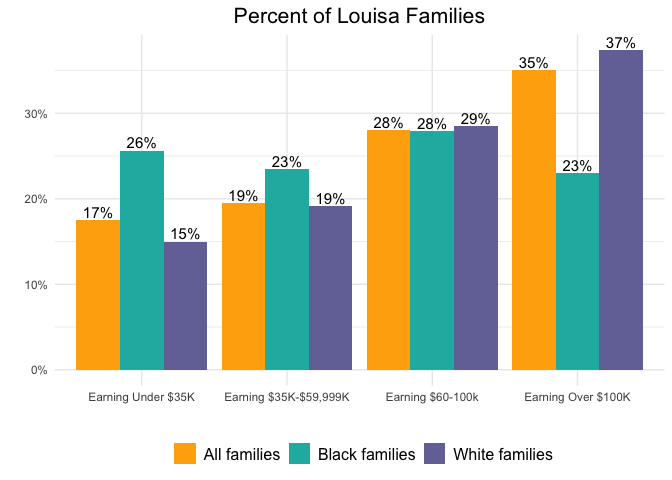
\includegraphics{orange-dot-test_files/figure-latex/unnamed-chunk-40-1} \end{center}

The maps below show the spatial relationship between income and
neighborhood. The color of each census tract in the county is based on
the median family income or the percent of families within the tract who
make less than \$35,000 a year. Having a higher percentage of struggling
families in a neighborhood has implications for the resources and
opportunities available to the families living there.

To see which neighborhoods in Louisa County have the highest and lowest
median family incomes, click on each tract to see its median income and
neighborhood names.

\hypertarget{median-family-income-in-louisa-county}{%
\subparagraph{Median Family Income in Louisa
County}\label{median-family-income-in-louisa-county}}

The lowest median family income is around the Town of Louisa, at
\$58,942. By contrast, the Zion Crossroads tract has the highest median
family income at \$102,829.

The following map shows the concentration of low-paid families. Similar
to the other counties, in Louisa County, the tract with the lowest
median family income also has the highest percentage of families making
less than \$35,000 per year.

\hypertarget{percent-of-families-making-under-35000-in-louisa-county}{%
\subparagraph{Percent of Families Making under \$35,000 in Louisa
County}\label{percent-of-families-making-under-35000-in-louisa-county}}

\protect\hyperlink{localities}{Return to Localities ↩︎}

\hypertarget{nelson-county}{%
\paragraph{Nelson County}\label{nelson-county}}

\hypertarget{nelson-county-1}{%
\subparagraph{Nelson County}\label{nelson-county-1}}

There are 4,372 families living in Nelson County. Of these, 812 (18.6\%)
do not earn enough to provide for their basic needs and the costs
associated with working.

Nelson County at a glance:

\begin{itemize}
\item
  Nelson ranks as the third least expensive locality for families in the
  region given the costs of housing and childcare.
\item
  In Nelson, the percent of Black families making under \$35,000 a year
  (29\%) is 12\% higher than the percent of white families making under
  \$35,000 a year (17\%).
\end{itemize}

\hypertarget{expenses-single-householder-2-children-1-toddler-6}{%
\subparagraph{Expenses: Single Householder + 2 Children (1
Toddler)}\label{expenses-single-householder-2-children-1-toddler-6}}

\global\setlength{\Oldarrayrulewidth}{\arrayrulewidth}

\global\setlength{\Oldtabcolsep}{\tabcolsep}

\setlength{\tabcolsep}{0pt}

\renewcommand*{\arraystretch}{1.5}



\providecommand{\ascline}[3]{\noalign{\global\arrayrulewidth #1}\arrayrulecolor[HTML]{#2}\cline{#3}}

\begin{longtable}[c]{|p{5.00in}|p{5.00in}|p{5.00in}|p{5.00in}}



\hhline{>{\arrayrulecolor[HTML]{666666}\global\arrayrulewidth=2pt}->{\arrayrulecolor[HTML]{666666}\global\arrayrulewidth=2pt}->{\arrayrulecolor[HTML]{666666}\global\arrayrulewidth=2pt}->{\arrayrulecolor[HTML]{666666}\global\arrayrulewidth=2pt}-}

\multicolumn{1}{>{\cellcolor[HTML]{FFFFFF}\centering}p{\dimexpr 5in+0\tabcolsep}}{\textcolor[HTML]{000000}{\fontsize{11}{11}\selectfont{Expense}}} & \multicolumn{1}{>{\cellcolor[HTML]{FFFFFF}\centering}p{\dimexpr 5in+0\tabcolsep}}{\textcolor[HTML]{000000}{\fontsize{11}{11}\selectfont{Annual}}} & \multicolumn{1}{>{\cellcolor[HTML]{FFFFFF}\centering}p{\dimexpr 5in+0\tabcolsep}}{\textcolor[HTML]{000000}{\fontsize{11}{11}\selectfont{Monthly}}} & \multicolumn{1}{>{\cellcolor[HTML]{FFFFFF}\centering}p{\dimexpr 5in+0\tabcolsep}}{\textcolor[HTML]{000000}{\fontsize{11}{11}\selectfont{Weekly}}} \\

\noalign{\global\arrayrulewidth 0pt}\arrayrulecolor[HTML]{000000}

\hhline{>{\arrayrulecolor[HTML]{666666}\global\arrayrulewidth=2pt}->{\arrayrulecolor[HTML]{666666}\global\arrayrulewidth=2pt}->{\arrayrulecolor[HTML]{666666}\global\arrayrulewidth=2pt}->{\arrayrulecolor[HTML]{666666}\global\arrayrulewidth=2pt}-}\endhead



\multicolumn{1}{>{\cellcolor[HTML]{FFFFFF}\centering}p{\dimexpr 5in+0\tabcolsep}}{\textcolor[HTML]{000000}{\fontsize{11}{11}\selectfont{Food}}} & \multicolumn{1}{>{\cellcolor[HTML]{FFFFFF}\centering}p{\dimexpr 5in+0\tabcolsep}}{\textcolor[HTML]{000000}{\fontsize{11}{11}\selectfont{6,630.0}}} & \multicolumn{1}{>{\cellcolor[HTML]{FFFFFF}\centering}p{\dimexpr 5in+0\tabcolsep}}{\textcolor[HTML]{000000}{\fontsize{11}{11}\selectfont{552.50}}} & \multicolumn{1}{>{\cellcolor[HTML]{FFFFFF}\centering}p{\dimexpr 5in+0\tabcolsep}}{\textcolor[HTML]{000000}{\fontsize{11}{11}\selectfont{127.50}}} \\

\noalign{\global\arrayrulewidth 0pt}\arrayrulecolor[HTML]{000000}

\hhline{>{\arrayrulecolor[HTML]{BEBEBE}\global\arrayrulewidth=1pt}->{\arrayrulecolor[HTML]{BEBEBE}\global\arrayrulewidth=1pt}->{\arrayrulecolor[HTML]{BEBEBE}\global\arrayrulewidth=1pt}->{\arrayrulecolor[HTML]{BEBEBE}\global\arrayrulewidth=1pt}-}



\multicolumn{1}{>{\cellcolor[HTML]{FFFFFF}\centering}p{\dimexpr 5in+0\tabcolsep}}{\textcolor[HTML]{000000}{\fontsize{11}{11}\selectfont{Clothing}}} & \multicolumn{1}{>{\cellcolor[HTML]{FFFFFF}\centering}p{\dimexpr 5in+0\tabcolsep}}{\textcolor[HTML]{000000}{\fontsize{11}{11}\selectfont{2,334.0}}} & \multicolumn{1}{>{\cellcolor[HTML]{FFFFFF}\centering}p{\dimexpr 5in+0\tabcolsep}}{\textcolor[HTML]{000000}{\fontsize{11}{11}\selectfont{194.50}}} & \multicolumn{1}{>{\cellcolor[HTML]{FFFFFF}\centering}p{\dimexpr 5in+0\tabcolsep}}{\textcolor[HTML]{000000}{\fontsize{11}{11}\selectfont{44.88}}} \\

\noalign{\global\arrayrulewidth 0pt}\arrayrulecolor[HTML]{000000}

\hhline{>{\arrayrulecolor[HTML]{BEBEBE}\global\arrayrulewidth=1pt}->{\arrayrulecolor[HTML]{BEBEBE}\global\arrayrulewidth=1pt}->{\arrayrulecolor[HTML]{BEBEBE}\global\arrayrulewidth=1pt}->{\arrayrulecolor[HTML]{BEBEBE}\global\arrayrulewidth=1pt}-}



\multicolumn{1}{>{\cellcolor[HTML]{FFFFFF}\centering}p{\dimexpr 5in+0\tabcolsep}}{\textcolor[HTML]{000000}{\fontsize{11}{11}\selectfont{Shelter}}} & \multicolumn{1}{>{\cellcolor[HTML]{FFFFFF}\centering}p{\dimexpr 5in+0\tabcolsep}}{\textcolor[HTML]{000000}{\fontsize{11}{11}\selectfont{15,168.0}}} & \multicolumn{1}{>{\cellcolor[HTML]{FFFFFF}\centering}p{\dimexpr 5in+0\tabcolsep}}{\textcolor[HTML]{000000}{\fontsize{11}{11}\selectfont{1,264.00}}} & \multicolumn{1}{>{\cellcolor[HTML]{FFFFFF}\centering}p{\dimexpr 5in+0\tabcolsep}}{\textcolor[HTML]{000000}{\fontsize{11}{11}\selectfont{291.69}}} \\

\noalign{\global\arrayrulewidth 0pt}\arrayrulecolor[HTML]{000000}

\hhline{>{\arrayrulecolor[HTML]{BEBEBE}\global\arrayrulewidth=1pt}->{\arrayrulecolor[HTML]{BEBEBE}\global\arrayrulewidth=1pt}->{\arrayrulecolor[HTML]{BEBEBE}\global\arrayrulewidth=1pt}->{\arrayrulecolor[HTML]{BEBEBE}\global\arrayrulewidth=1pt}-}



\multicolumn{1}{>{\cellcolor[HTML]{FFFFFF}\centering}p{\dimexpr 5in+0\tabcolsep}}{\textcolor[HTML]{000000}{\fontsize{11}{11}\selectfont{Utilities}}} & \multicolumn{1}{>{\cellcolor[HTML]{FFFFFF}\centering}p{\dimexpr 5in+0\tabcolsep}}{\textcolor[HTML]{000000}{\fontsize{11}{11}\selectfont{3,325.0}}} & \multicolumn{1}{>{\cellcolor[HTML]{FFFFFF}\centering}p{\dimexpr 5in+0\tabcolsep}}{\textcolor[HTML]{000000}{\fontsize{11}{11}\selectfont{277.08}}} & \multicolumn{1}{>{\cellcolor[HTML]{FFFFFF}\centering}p{\dimexpr 5in+0\tabcolsep}}{\textcolor[HTML]{000000}{\fontsize{11}{11}\selectfont{63.94}}} \\

\noalign{\global\arrayrulewidth 0pt}\arrayrulecolor[HTML]{000000}

\hhline{>{\arrayrulecolor[HTML]{BEBEBE}\global\arrayrulewidth=1pt}->{\arrayrulecolor[HTML]{BEBEBE}\global\arrayrulewidth=1pt}->{\arrayrulecolor[HTML]{BEBEBE}\global\arrayrulewidth=1pt}->{\arrayrulecolor[HTML]{BEBEBE}\global\arrayrulewidth=1pt}-}



\multicolumn{1}{>{\cellcolor[HTML]{FFFFFF}\centering}p{\dimexpr 5in+0\tabcolsep}}{\textcolor[HTML]{000000}{\fontsize{11}{11}\selectfont{Necessary\ Costs}}} & \multicolumn{1}{>{\cellcolor[HTML]{FFFFFF}\centering}p{\dimexpr 5in+0\tabcolsep}}{\textcolor[HTML]{000000}{\fontsize{11}{11}\selectfont{5,491.4}}} & \multicolumn{1}{>{\cellcolor[HTML]{FFFFFF}\centering}p{\dimexpr 5in+0\tabcolsep}}{\textcolor[HTML]{000000}{\fontsize{11}{11}\selectfont{457.62}}} & \multicolumn{1}{>{\cellcolor[HTML]{FFFFFF}\centering}p{\dimexpr 5in+0\tabcolsep}}{\textcolor[HTML]{000000}{\fontsize{11}{11}\selectfont{105.60}}} \\

\noalign{\global\arrayrulewidth 0pt}\arrayrulecolor[HTML]{000000}

\hhline{>{\arrayrulecolor[HTML]{BEBEBE}\global\arrayrulewidth=1pt}->{\arrayrulecolor[HTML]{BEBEBE}\global\arrayrulewidth=1pt}->{\arrayrulecolor[HTML]{BEBEBE}\global\arrayrulewidth=1pt}->{\arrayrulecolor[HTML]{BEBEBE}\global\arrayrulewidth=1pt}-}



\multicolumn{1}{>{\cellcolor[HTML]{FFAD0A}\centering}p{\dimexpr 5in+0\tabcolsep}}{\textcolor[HTML]{000000}{\fontsize{11}{11}\selectfont{Survival\ Expenses}}} & \multicolumn{1}{>{\cellcolor[HTML]{FFAD0A}\centering}p{\dimexpr 5in+0\tabcolsep}}{\textcolor[HTML]{000000}{\fontsize{11}{11}\selectfont{32,948.4}}} & \multicolumn{1}{>{\cellcolor[HTML]{FFAD0A}\centering}p{\dimexpr 5in+0\tabcolsep}}{\textcolor[HTML]{000000}{\fontsize{11}{11}\selectfont{2,745.70}}} & \multicolumn{1}{>{\cellcolor[HTML]{FFAD0A}\centering}p{\dimexpr 5in+0\tabcolsep}}{\textcolor[HTML]{000000}{\fontsize{11}{11}\selectfont{633.62}}} \\

\noalign{\global\arrayrulewidth 0pt}\arrayrulecolor[HTML]{000000}

\hhline{>{\arrayrulecolor[HTML]{BEBEBE}\global\arrayrulewidth=1pt}->{\arrayrulecolor[HTML]{BEBEBE}\global\arrayrulewidth=1pt}->{\arrayrulecolor[HTML]{BEBEBE}\global\arrayrulewidth=1pt}->{\arrayrulecolor[HTML]{BEBEBE}\global\arrayrulewidth=1pt}-}



\multicolumn{1}{>{\cellcolor[HTML]{FFFFFF}\centering}p{\dimexpr 5in+0\tabcolsep}}{\textcolor[HTML]{000000}{\fontsize{11}{11}\selectfont{Childcare}}} & \multicolumn{1}{>{\cellcolor[HTML]{FFFFFF}\centering}p{\dimexpr 5in+0\tabcolsep}}{\textcolor[HTML]{000000}{\fontsize{11}{11}\selectfont{14,040.0}}} & \multicolumn{1}{>{\cellcolor[HTML]{FFFFFF}\centering}p{\dimexpr 5in+0\tabcolsep}}{\textcolor[HTML]{000000}{\fontsize{11}{11}\selectfont{1,170.00}}} & \multicolumn{1}{>{\cellcolor[HTML]{FFFFFF}\centering}p{\dimexpr 5in+0\tabcolsep}}{\textcolor[HTML]{000000}{\fontsize{11}{11}\selectfont{270.00}}} \\

\noalign{\global\arrayrulewidth 0pt}\arrayrulecolor[HTML]{000000}

\hhline{>{\arrayrulecolor[HTML]{BEBEBE}\global\arrayrulewidth=1pt}->{\arrayrulecolor[HTML]{BEBEBE}\global\arrayrulewidth=1pt}->{\arrayrulecolor[HTML]{BEBEBE}\global\arrayrulewidth=1pt}->{\arrayrulecolor[HTML]{BEBEBE}\global\arrayrulewidth=1pt}-}



\multicolumn{1}{>{\cellcolor[HTML]{FFFFFF}\centering}p{\dimexpr 5in+0\tabcolsep}}{\textcolor[HTML]{000000}{\fontsize{11}{11}\selectfont{Transportation}}} & \multicolumn{1}{>{\cellcolor[HTML]{FFFFFF}\centering}p{\dimexpr 5in+0\tabcolsep}}{\textcolor[HTML]{000000}{\fontsize{11}{11}\selectfont{3,996.0}}} & \multicolumn{1}{>{\cellcolor[HTML]{FFFFFF}\centering}p{\dimexpr 5in+0\tabcolsep}}{\textcolor[HTML]{000000}{\fontsize{11}{11}\selectfont{333.00}}} & \multicolumn{1}{>{\cellcolor[HTML]{FFFFFF}\centering}p{\dimexpr 5in+0\tabcolsep}}{\textcolor[HTML]{000000}{\fontsize{11}{11}\selectfont{76.85}}} \\

\noalign{\global\arrayrulewidth 0pt}\arrayrulecolor[HTML]{000000}

\hhline{>{\arrayrulecolor[HTML]{BEBEBE}\global\arrayrulewidth=1pt}->{\arrayrulecolor[HTML]{BEBEBE}\global\arrayrulewidth=1pt}->{\arrayrulecolor[HTML]{BEBEBE}\global\arrayrulewidth=1pt}->{\arrayrulecolor[HTML]{BEBEBE}\global\arrayrulewidth=1pt}-}



\multicolumn{1}{>{\cellcolor[HTML]{EE6100}\centering}p{\dimexpr 5in+0\tabcolsep}}{\textcolor[HTML]{FFFFFF}{\fontsize{11}{11}\selectfont{Total\ Expenses}}} & \multicolumn{1}{>{\cellcolor[HTML]{EE6100}\centering}p{\dimexpr 5in+0\tabcolsep}}{\textcolor[HTML]{FFFFFF}{\fontsize{11}{11}\selectfont{50,984.4}}} & \multicolumn{1}{>{\cellcolor[HTML]{EE6100}\centering}p{\dimexpr 5in+0\tabcolsep}}{\textcolor[HTML]{FFFFFF}{\fontsize{11}{11}\selectfont{4,116.20}}} & \multicolumn{1}{>{\cellcolor[HTML]{EE6100}\centering}p{\dimexpr 5in+0\tabcolsep}}{\textcolor[HTML]{FFFFFF}{\fontsize{11}{11}\selectfont{949.89}}} \\

\noalign{\global\arrayrulewidth 0pt}\arrayrulecolor[HTML]{000000}

\hhline{>{\arrayrulecolor[HTML]{666666}\global\arrayrulewidth=2pt}->{\arrayrulecolor[HTML]{666666}\global\arrayrulewidth=2pt}->{\arrayrulecolor[HTML]{666666}\global\arrayrulewidth=2pt}->{\arrayrulecolor[HTML]{666666}\global\arrayrulewidth=2pt}-}



\end{longtable}



\arrayrulecolor[HTML]{000000}

\global\setlength{\arrayrulewidth}{\Oldarrayrulewidth}

\global\setlength{\tabcolsep}{\Oldtabcolsep}

\renewcommand*{\arraystretch}{1}

\hypertarget{breakdown-of-families-making-under-35000-in-nelson-county}{%
\subparagraph{Breakdown of Families Making under \$35,000 in Nelson
County}\label{breakdown-of-families-making-under-35000-in-nelson-county}}

\global\setlength{\Oldarrayrulewidth}{\arrayrulewidth}

\global\setlength{\Oldtabcolsep}{\tabcolsep}

\setlength{\tabcolsep}{0pt}

\renewcommand*{\arraystretch}{1.5}



\providecommand{\ascline}[3]{\noalign{\global\arrayrulewidth #1}\arrayrulecolor[HTML]{#2}\cline{#3}}

\begin{longtable}[c]{|p{5.00in}|p{5.00in}|p{5.00in}|p{5.00in}}



\hhline{>{\arrayrulecolor[HTML]{666666}\global\arrayrulewidth=2pt}->{\arrayrulecolor[HTML]{666666}\global\arrayrulewidth=2pt}->{\arrayrulecolor[HTML]{666666}\global\arrayrulewidth=2pt}->{\arrayrulecolor[HTML]{666666}\global\arrayrulewidth=2pt}-}

\multicolumn{1}{>{\cellcolor[HTML]{FFFFFF}\centering}p{\dimexpr 5in+0\tabcolsep}}{\textcolor[HTML]{000000}{\fontsize{11}{11}\selectfont{Income}}} & \multicolumn{1}{>{\cellcolor[HTML]{FFFFFF}\centering}p{\dimexpr 5in+0\tabcolsep}}{\textcolor[HTML]{000000}{\fontsize{11}{11}\selectfont{Number}}} & \multicolumn{1}{>{\cellcolor[HTML]{FFFFFF}\centering}p{\dimexpr 5in+0\tabcolsep}}{\textcolor[HTML]{000000}{\fontsize{11}{11}\selectfont{Percent}}} & \multicolumn{1}{>{\cellcolor[HTML]{FFFFFF}\centering}p{\dimexpr 5in+0\tabcolsep}}{\textcolor[HTML]{000000}{\fontsize{11}{11}\selectfont{Cumulative}}} \\

\noalign{\global\arrayrulewidth 0pt}\arrayrulecolor[HTML]{000000}

\hhline{>{\arrayrulecolor[HTML]{666666}\global\arrayrulewidth=2pt}->{\arrayrulecolor[HTML]{666666}\global\arrayrulewidth=2pt}->{\arrayrulecolor[HTML]{666666}\global\arrayrulewidth=2pt}->{\arrayrulecolor[HTML]{666666}\global\arrayrulewidth=2pt}-}\endhead



\multicolumn{1}{>{\cellcolor[HTML]{FFFFFF}\centering}p{\dimexpr 5in+0\tabcolsep}}{\textcolor[HTML]{000000}{\fontsize{11}{11}\selectfont{\$0\ -\ \$9,999}}} & \multicolumn{1}{>{\cellcolor[HTML]{FFFFFF}\centering}p{\dimexpr 5in+0\tabcolsep}}{\textcolor[HTML]{000000}{\fontsize{11}{11}\selectfont{175}}} & \multicolumn{1}{>{\cellcolor[HTML]{FFFFFF}\centering}p{\dimexpr 5in+0\tabcolsep}}{\textcolor[HTML]{000000}{\fontsize{11}{11}\selectfont{22\%}}} & \multicolumn{1}{>{\cellcolor[HTML]{FFAD0A}\centering}p{\dimexpr 5in+0\tabcolsep}}{} \\

\noalign{\global\arrayrulewidth 0pt}\arrayrulecolor[HTML]{000000}

\hhline{>{\arrayrulecolor[HTML]{BEBEBE}\global\arrayrulewidth=1pt}->{\arrayrulecolor[HTML]{BEBEBE}\global\arrayrulewidth=1pt}->{\arrayrulecolor[HTML]{BEBEBE}\global\arrayrulewidth=1pt}->{\arrayrulecolor[HTML]{FFAD0A}\global\arrayrulewidth=1pt}-}



\multicolumn{1}{>{\cellcolor[HTML]{FFFFFF}\centering}p{\dimexpr 5in+0\tabcolsep}}{\textcolor[HTML]{000000}{\fontsize{11}{11}\selectfont{\$10,000\ -\ \$14,999}}} & \multicolumn{1}{>{\cellcolor[HTML]{FFFFFF}\centering}p{\dimexpr 5in+0\tabcolsep}}{\textcolor[HTML]{000000}{\fontsize{11}{11}\selectfont{49}}} & \multicolumn{1}{>{\cellcolor[HTML]{FFFFFF}\centering}p{\dimexpr 5in+0\tabcolsep}}{\textcolor[HTML]{000000}{\fontsize{11}{11}\selectfont{6\%}}} & \multicolumn{1}{>{\cellcolor[HTML]{FFAD0A}\centering}p{\dimexpr 5in+0\tabcolsep}}{\multirow[c]{-2}{*}{\parbox{5in}{\textcolor[HTML]{000000}{\fontsize{11}{11}\selectfont{28\%}}}}} \\

\noalign{\global\arrayrulewidth 0pt}\arrayrulecolor[HTML]{000000}

\hhline{>{\arrayrulecolor[HTML]{BEBEBE}\global\arrayrulewidth=1pt}->{\arrayrulecolor[HTML]{BEBEBE}\global\arrayrulewidth=1pt}->{\arrayrulecolor[HTML]{BEBEBE}\global\arrayrulewidth=1pt}->{\arrayrulecolor[HTML]{BEBEBE}\global\arrayrulewidth=1pt}-}



\multicolumn{1}{>{\cellcolor[HTML]{FFFFFF}\centering}p{\dimexpr 5in+0\tabcolsep}}{\textcolor[HTML]{000000}{\fontsize{11}{11}\selectfont{\$15,000\ -\ \$24,999}}} & \multicolumn{1}{>{\cellcolor[HTML]{FFFFFF}\centering}p{\dimexpr 5in+0\tabcolsep}}{\textcolor[HTML]{000000}{\fontsize{11}{11}\selectfont{186}}} & \multicolumn{1}{>{\cellcolor[HTML]{FFFFFF}\centering}p{\dimexpr 5in+0\tabcolsep}}{\textcolor[HTML]{000000}{\fontsize{11}{11}\selectfont{23\%}}} & \multicolumn{1}{>{\cellcolor[HTML]{EE6100}\centering}p{\dimexpr 5in+0\tabcolsep}}{} \\

\noalign{\global\arrayrulewidth 0pt}\arrayrulecolor[HTML]{000000}

\hhline{>{\arrayrulecolor[HTML]{BEBEBE}\global\arrayrulewidth=1pt}->{\arrayrulecolor[HTML]{BEBEBE}\global\arrayrulewidth=1pt}->{\arrayrulecolor[HTML]{BEBEBE}\global\arrayrulewidth=1pt}->{\arrayrulecolor[HTML]{EE6100}\global\arrayrulewidth=1pt}-}



\multicolumn{1}{>{\cellcolor[HTML]{FFFFFF}\centering}p{\dimexpr 5in+0\tabcolsep}}{\textcolor[HTML]{000000}{\fontsize{11}{11}\selectfont{\$25,000\ -\ \$34,999}}} & \multicolumn{1}{>{\cellcolor[HTML]{FFFFFF}\centering}p{\dimexpr 5in+0\tabcolsep}}{\textcolor[HTML]{000000}{\fontsize{11}{11}\selectfont{402}}} & \multicolumn{1}{>{\cellcolor[HTML]{FFFFFF}\centering}p{\dimexpr 5in+0\tabcolsep}}{\textcolor[HTML]{000000}{\fontsize{11}{11}\selectfont{50\%}}} & \multicolumn{1}{>{\cellcolor[HTML]{EE6100}\centering}p{\dimexpr 5in+0\tabcolsep}}{\multirow[c]{-2}{*}{\parbox{5in}{\textcolor[HTML]{FFFFFF}{\fontsize{11}{11}\selectfont{73\%}}}}} \\

\noalign{\global\arrayrulewidth 0pt}\arrayrulecolor[HTML]{000000}

\hhline{>{\arrayrulecolor[HTML]{BEBEBE}\global\arrayrulewidth=1pt}->{\arrayrulecolor[HTML]{BEBEBE}\global\arrayrulewidth=1pt}->{\arrayrulecolor[HTML]{BEBEBE}\global\arrayrulewidth=1pt}->{\arrayrulecolor[HTML]{BEBEBE}\global\arrayrulewidth=1pt}-}



\multicolumn{1}{>{\cellcolor[HTML]{FFFFFF}\centering}p{\dimexpr 5in+0\tabcolsep}}{\textcolor[HTML]{000000}{\fontsize{11}{11}\selectfont{Total}}} & \multicolumn{1}{>{\cellcolor[HTML]{FFFFFF}\centering}p{\dimexpr 5in+0\tabcolsep}}{\textcolor[HTML]{000000}{\fontsize{11}{11}\selectfont{812}}} & \multicolumn{2}{>{\cellcolor[HTML]{FFFFFF}\centering}p{\dimexpr 10in+2\tabcolsep}}{\textcolor[HTML]{000000}{\fontsize{11}{11}\selectfont{100\%}}} \\

\noalign{\global\arrayrulewidth 0pt}\arrayrulecolor[HTML]{000000}

\hhline{>{\arrayrulecolor[HTML]{666666}\global\arrayrulewidth=2pt}->{\arrayrulecolor[HTML]{666666}\global\arrayrulewidth=2pt}->{\arrayrulecolor[HTML]{666666}\global\arrayrulewidth=2pt}->{\arrayrulecolor[HTML]{666666}\global\arrayrulewidth=2pt}-}



\end{longtable}



\arrayrulecolor[HTML]{000000}

\global\setlength{\arrayrulewidth}{\Oldarrayrulewidth}

\global\setlength{\tabcolsep}{\Oldtabcolsep}

\renewcommand*{\arraystretch}{1}

As this table shows, 73\% of the families who cannot meet their basic
needs earn between \$15,000-\$35,000 annually. This strongly suggests
they are working, but not earning the wages or not getting the hours
they need to support their families.

The figure below shows the distribution of families in various pay
ranges, disaggregated by race. In a world with racial equity in income,
the bars for all families would be equal in height. In Nelson County,
Black families are over-represented at the low end of the pay range
(under \$35,000) and under-represented at the high end of the pay range
(over \$100k/year). In other words, relative to white families, Black
families are more likely to be paid insufficient wages and less likely
to be high-earning.

\hypertarget{income-distribution-of-black-and-white-families-in-nelson-county}{%
\subparagraph{Income Distribution of Black and White Families in Nelson
County}\label{income-distribution-of-black-and-white-families-in-nelson-county}}

\begin{center}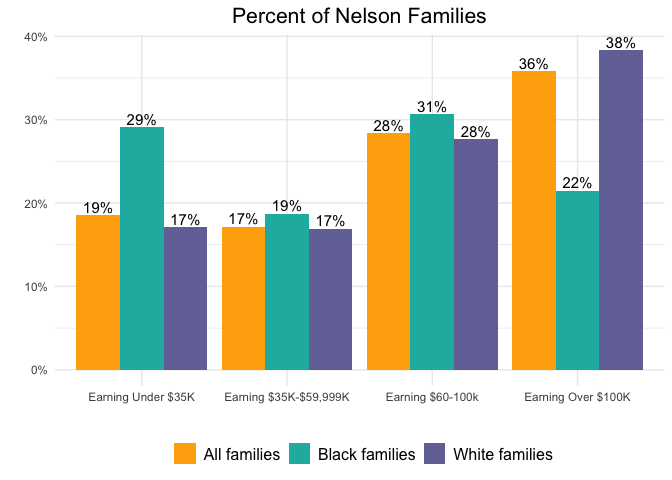
\includegraphics{orange-dot-test_files/figure-latex/unnamed-chunk-46-1} \end{center}

The maps below show the spatial relationship between income and
neighborhood. The color of each census tract in the county is based on
the median family income or the percent of families within the tract who
make less than \$35,000 per year. Having a higher percentage of
struggling families in an area has implications for the resources and
opportunities available to the families living there.

To see which neighborhoods in Nelson County have the highest and lowest
median family incomes, click on each tract to see its median income and
neighborhood names.

\hypertarget{median-family-income-in-nelson-county}{%
\subparagraph{Median Family Income in Nelson
County}\label{median-family-income-in-nelson-county}}

The Lovingston tract has the lowest median family incomes at \$67,656.
By contrast, the Wintergreen-Rockfish Valley tract has the highest
median family income at \$105,938.

The following map shows the concentration of low-paid families. Similar
to the other counties, in Fluvanna County, the tract with the lowest
median family income also has the highest percentage of families making
less than \$35,000 yearly.

\hypertarget{percent-of-families-making-under-35000-in-nelson-county}{%
\subparagraph{Percent of Families Making under \$35,000 in Nelson
County}\label{percent-of-families-making-under-35000-in-nelson-county}}

\protect\hyperlink{localities}{Return to Localities ↩︎}

\hypertarget{conclusion}{%
\subsection{Conclusion}\label{conclusion}}

\begin{quote}
``When someone works for less pay than she can live on---when, for
example, she goes hungry so that you can eat more cheaply and
conveniently---then she has made a great sacrifice for you, she has made
you a gift of some part of her abilities, her health, and her life. The
`working poor,' as they are approvingly termed, are in fact the major
philanthropists of our society.''

--- Barbara Ehrenreich.\footnote{Barbara Ehrenreich (2001). Nickel and
  Dimed: On (Not) Getting By in America. Metropolitan Books.}
\end{quote}

Based on data collected from 2016-2020, at least 9,413 families in the
larger Charlottesville region make less than \$35,000 a year, far below
what's necessary to afford the essentials of life---food, shelter,
clothing and utilities---and additional costs incurred by working. These
families reside throughout our region. While Albemarle County, Louisa
County, and the City of Charlottesville have the highest number of
struggling families, Buckingham County, the City of Charlottesville, and
Nelson County have the highest percent of struggling families. And
across each locality in our region, the percent of Black families making
less than \$35,000 exceeds the percent of white families making less
than \$35,000. Despite working equally hard, the labor of Black families
in the Charlottesville region is not equally valued.

We are making steady progress in decreasing the number, and percent, of
families making under \$35,000 annually. The cost of living, however,
continues to rise---currently working families with a toddler and a
preschooler need between \$42,000 and \$50,000 to be self-sufficient,
based largely on the cost of housing and childcare. And inflationary
forces can rapidly shift the fortunes of struggling families.

We consider this estimate of nearly 10,000 struggling families a
minimum, and while lower than that found in prior Orange Dot Reports, it
is too many. No one should labor full time for insufficient wages, and
our treatment of our essential workers must improve; their labor should
not be a sacrifice for our comfort. The pandemic showed us how essential
is the labor of workers who keep our shelves stocked and our stores
open, who help care for our children and our parents, who ensure our
transportation and logistics systems for people and goods keep running.
Our dependence on one another to keep society functioning has rarely
been so clear. That same interdependence demands we do more to help
struggling families reach positions of greater financial security.

The second part of this report, to be released in the spring, will
review community efforts to provide families with the better paying jobs
they need to succeed, including a review of the approach and progress of
the pioneering Network2Work framework, as well as opportunities to
create more pipelines into stable regional employers. The spring release
will further consider approaches to addressing the rising costs that
threaten to increase the number of families who struggle in our
region---housing and access to capital, child care and early education.
Promoting the well-being and thriving of all of our neighbors, and, in
turn, of our community, will require sustained, cooperative, and
intentional effort by individuals, government and non-governmental
organizations, powerful employers, and more. In short, by our local,
state, and national economic actors and by our public and civic society.

\hypertarget{notes}{%
\subsection{Notes}\label{notes}}

\end{document}
